% Options for packages loaded elsewhere
\PassOptionsToPackage{unicode}{hyperref}
\PassOptionsToPackage{hyphens}{url}
%
\documentclass[
]{article}
\usepackage{amsmath,amssymb}
\usepackage{iftex}
\ifPDFTeX
  \usepackage[T1]{fontenc}
  \usepackage[utf8]{inputenc}
  \usepackage{textcomp} % provide euro and other symbols
\else % if luatex or xetex
  \usepackage{unicode-math} % this also loads fontspec
  \defaultfontfeatures{Scale=MatchLowercase}
  \defaultfontfeatures[\rmfamily]{Ligatures=TeX,Scale=1}
\fi
\usepackage{lmodern}
\ifPDFTeX\else
  % xetex/luatex font selection
\fi
% Use upquote if available, for straight quotes in verbatim environments
\IfFileExists{upquote.sty}{\usepackage{upquote}}{}
\IfFileExists{microtype.sty}{% use microtype if available
  \usepackage[]{microtype}
  \UseMicrotypeSet[protrusion]{basicmath} % disable protrusion for tt fonts
}{}
\makeatletter
\@ifundefined{KOMAClassName}{% if non-KOMA class
  \IfFileExists{parskip.sty}{%
    \usepackage{parskip}
  }{% else
    \setlength{\parindent}{0pt}
    \setlength{\parskip}{6pt plus 2pt minus 1pt}}
}{% if KOMA class
  \KOMAoptions{parskip=half}}
\makeatother
\usepackage{xcolor}
\usepackage[margin=1in]{geometry}
\usepackage{color}
\usepackage{fancyvrb}
\newcommand{\VerbBar}{|}
\newcommand{\VERB}{\Verb[commandchars=\\\{\}]}
\DefineVerbatimEnvironment{Highlighting}{Verbatim}{commandchars=\\\{\}}
% Add ',fontsize=\small' for more characters per line
\usepackage{framed}
\definecolor{shadecolor}{RGB}{248,248,248}
\newenvironment{Shaded}{\begin{snugshade}}{\end{snugshade}}
\newcommand{\AlertTok}[1]{\textcolor[rgb]{0.94,0.16,0.16}{#1}}
\newcommand{\AnnotationTok}[1]{\textcolor[rgb]{0.56,0.35,0.01}{\textbf{\textit{#1}}}}
\newcommand{\AttributeTok}[1]{\textcolor[rgb]{0.13,0.29,0.53}{#1}}
\newcommand{\BaseNTok}[1]{\textcolor[rgb]{0.00,0.00,0.81}{#1}}
\newcommand{\BuiltInTok}[1]{#1}
\newcommand{\CharTok}[1]{\textcolor[rgb]{0.31,0.60,0.02}{#1}}
\newcommand{\CommentTok}[1]{\textcolor[rgb]{0.56,0.35,0.01}{\textit{#1}}}
\newcommand{\CommentVarTok}[1]{\textcolor[rgb]{0.56,0.35,0.01}{\textbf{\textit{#1}}}}
\newcommand{\ConstantTok}[1]{\textcolor[rgb]{0.56,0.35,0.01}{#1}}
\newcommand{\ControlFlowTok}[1]{\textcolor[rgb]{0.13,0.29,0.53}{\textbf{#1}}}
\newcommand{\DataTypeTok}[1]{\textcolor[rgb]{0.13,0.29,0.53}{#1}}
\newcommand{\DecValTok}[1]{\textcolor[rgb]{0.00,0.00,0.81}{#1}}
\newcommand{\DocumentationTok}[1]{\textcolor[rgb]{0.56,0.35,0.01}{\textbf{\textit{#1}}}}
\newcommand{\ErrorTok}[1]{\textcolor[rgb]{0.64,0.00,0.00}{\textbf{#1}}}
\newcommand{\ExtensionTok}[1]{#1}
\newcommand{\FloatTok}[1]{\textcolor[rgb]{0.00,0.00,0.81}{#1}}
\newcommand{\FunctionTok}[1]{\textcolor[rgb]{0.13,0.29,0.53}{\textbf{#1}}}
\newcommand{\ImportTok}[1]{#1}
\newcommand{\InformationTok}[1]{\textcolor[rgb]{0.56,0.35,0.01}{\textbf{\textit{#1}}}}
\newcommand{\KeywordTok}[1]{\textcolor[rgb]{0.13,0.29,0.53}{\textbf{#1}}}
\newcommand{\NormalTok}[1]{#1}
\newcommand{\OperatorTok}[1]{\textcolor[rgb]{0.81,0.36,0.00}{\textbf{#1}}}
\newcommand{\OtherTok}[1]{\textcolor[rgb]{0.56,0.35,0.01}{#1}}
\newcommand{\PreprocessorTok}[1]{\textcolor[rgb]{0.56,0.35,0.01}{\textit{#1}}}
\newcommand{\RegionMarkerTok}[1]{#1}
\newcommand{\SpecialCharTok}[1]{\textcolor[rgb]{0.81,0.36,0.00}{\textbf{#1}}}
\newcommand{\SpecialStringTok}[1]{\textcolor[rgb]{0.31,0.60,0.02}{#1}}
\newcommand{\StringTok}[1]{\textcolor[rgb]{0.31,0.60,0.02}{#1}}
\newcommand{\VariableTok}[1]{\textcolor[rgb]{0.00,0.00,0.00}{#1}}
\newcommand{\VerbatimStringTok}[1]{\textcolor[rgb]{0.31,0.60,0.02}{#1}}
\newcommand{\WarningTok}[1]{\textcolor[rgb]{0.56,0.35,0.01}{\textbf{\textit{#1}}}}
\usepackage{longtable,booktabs,array}
\usepackage{calc} % for calculating minipage widths
% Correct order of tables after \paragraph or \subparagraph
\usepackage{etoolbox}
\makeatletter
\patchcmd\longtable{\par}{\if@noskipsec\mbox{}\fi\par}{}{}
\makeatother
% Allow footnotes in longtable head/foot
\IfFileExists{footnotehyper.sty}{\usepackage{footnotehyper}}{\usepackage{footnote}}
\makesavenoteenv{longtable}
\usepackage{graphicx}
\makeatletter
\def\maxwidth{\ifdim\Gin@nat@width>\linewidth\linewidth\else\Gin@nat@width\fi}
\def\maxheight{\ifdim\Gin@nat@height>\textheight\textheight\else\Gin@nat@height\fi}
\makeatother
% Scale images if necessary, so that they will not overflow the page
% margins by default, and it is still possible to overwrite the defaults
% using explicit options in \includegraphics[width, height, ...]{}
\setkeys{Gin}{width=\maxwidth,height=\maxheight,keepaspectratio}
% Set default figure placement to htbp
\makeatletter
\def\fps@figure{htbp}
\makeatother
\setlength{\emergencystretch}{3em} % prevent overfull lines
\providecommand{\tightlist}{%
  \setlength{\itemsep}{0pt}\setlength{\parskip}{0pt}}
\setcounter{secnumdepth}{5}
\usepackage{booktabs}
\usepackage{caption}
\usepackage{natbib}
\usepackage{amsmath}
\usepackage{inputenc}

\parindent=0cm
%\itemsep=0.7cm
\parskip=0.2cm
%\baselineskip=1cm
\textheight=22.5cm \textwidth=16cm \setlength{\oddsidemargin}{0cm}
\setlength{\evensidemargin}{0cm} \setlength{\topmargin}{-1cm}
\newcommand{\bepsilon}{\boldsymbol \epsilon}
\newcommand{\bpsi}{\boldsymbol \psi}
\newcommand{\bmu}{\boldsymbol \mu}
\newcommand{\cl}{ℓ}
\newcommand{\bx}{\boldsymbol x}
\newcommand{\bX}{\boldsymbol X}
\newcommand{\bZERO}{\boldsymbol 0}
\newcommand{\bONE}{\boldsymbol 1}
\newcommand{\tr}{\mbox{tr}}
\newcommand{\bb}{\boldsymbol b}
\newcommand{\hatbb}{\widehat{\bb}}
\newcommand{\hatb}{\widehat{b}}
\newcommand{\bc}{\boldsymbol c}
\newcommand{\bC}{\boldsymbol C}
\newcommand{\bD}{\boldsymbol D}
\newcommand{\be}{\boldsymbol e}
\newcommand{\bH}{\boldsymbol H}
\newcommand{\bI}{\boldsymbol I}
\newcommand{\bl}{\boldsymbol l}
\newcommand{\bL}{\boldsymbol L}
\newcommand{\bM}{\boldsymbol M}
\newcommand{\bp}{\boldsymbol p}
\newcommand{\bP}{\boldsymbol P}
\newcommand{\br}{\boldsymbol r}
\newcommand{\bR}{\boldsymbol R}
\newcommand{\bt}{\boldsymbol t}
\newcommand{\bT}{\boldsymbol T}
\newcommand{\bu}{\boldsymbol u}
\newcommand{\bU}{\boldsymbol U}
\newcommand{\by}{\boldsymbol y}
\newcommand{\bY}{\boldsymbol Y}
\newcommand{\bZ}{\boldsymbol Z}
\newcommand{\bV}{\boldsymbol V}
\newcommand{\bW}{\boldsymbol W}
\newcommand{\bz}{\boldsymbol z}
\newcommand{\tildey}{\widetilde{y}}
\newcommand{\tildeby}{\widetilde{\by}}
\newcommand{\tildetheta}{\widetilde{\theta}}
\newcommand{\tildemu}{\widetilde{\mu}}
\newcommand{\haty}{\widehat{y}}
\newcommand{\hatby}{\widehat{\by}}
\newcommand{\hatalpha}{\widehat{\alpha}}
\newcommand{\balpha}{\boldsymbol \alpha}
\newcommand{\hatbalpha}{\widehat{\balpha}}
\newcommand{\bbeta}{\boldsymbol \beta}
\newcommand{\hatbeta}{\widehat{\beta}}
\newcommand{\hatpi}{\widehat{\pi}}
\newcommand{\hatbbeta}{\widehat{\bbeta}}
\newcommand{\bgamma}{\boldsymbol \gamma}
\newcommand{\hatmu}{\widehat{\mu}}
\newcommand{\hatbmu}{\widehat{\bmu}}
\newcommand{\hatsigma}{\widehat{\sigma}}
\newcommand{\hatlambda}{\widehat{\lambda}}
\newcommand{\hatbLambda}{\widehat{\bLambda}}
\newcommand{\btheta}{\boldsymbol \theta}
\newcommand{\hatbtheta}{\widehat{\btheta}}
\newcommand{\bLambda}{\boldsymbol \Lambda}
\newcommand{\bvarepsi}{\boldsymbol \varepsilon}
\newcommand{\bpi}{\boldsymbol \pi}
\newcommand{\Sres}{SS_{\mbox{res}}}
\newcommand{\Sreg}{SS_{\mbox{reg}}}
\newcommand{\Stotal}{SS_{\mbox{T}}}
\newcommand{\MSres}{MS_{\mbox{res}}}
\newcommand{\MSreg}{MS_{\mbox{reg}}}
\renewcommand{\figurename}{Figura}
\renewcommand{\tablename}{Tabla}
\ifLuaTeX
  \usepackage{selnolig}  % disable illegal ligatures
\fi
\usepackage[]{natbib}
\bibliographystyle{apalike}
\IfFileExists{bookmark.sty}{\usepackage{bookmark}}{\usepackage{hyperref}}
\IfFileExists{xurl.sty}{\usepackage{xurl}}{} % add URL line breaks if available
\urlstyle{same}
\hypersetup{
  pdftitle={Notas de clase: Modelo lineal general I},
  pdfauthor={Alvaro J. Flórez},
  hidelinks,
  pdfcreator={LaTeX via pandoc}}

\title{Notas de clase: Modelo lineal general I}
\author{Alvaro J. Flórez}
\date{2024-02-21}

\begin{document}
\maketitle

{
\setcounter{tocdepth}{2}
\tableofcontents
}
\hypertarget{introducciuxf3n}{%
\section*{Introducción}\label{introducciuxf3n}}
\addcontentsline{toc}{section}{Introducción}

Estas son las notas de clase del curso Modelo Lineal General I. Las temáticas que se tratan son:

\begin{enumerate}
\def\labelenumi{\arabic{enumi}.}
\tightlist
\item
  Modelo lineal simple
\item
  Modelo lineal múltiple
\item
  Evaluación de los supuestos del modelo lineal
\item
  Transformaciones y mínimos cuadrados ponderados
\item
  Evaluación de puntos influyentes y atípicos
\end{enumerate}

Tenga en cuenta que el propósito de estas notas de clase no es reemplazar los textos guías. Para el estudio más detallado de los temas revisados, se recomiendan las siguientes lecturas:

\begin{itemize}
\tightlist
\item
  \emph{Introduction to Linear Regression Analysis}, Fifth Ed., 2012, by Montgomery, D. C., Peck, E. A. and Vining, G. G. \textbf{(Texto guía)}
\item
  \emph{Applied Regression Analysis}, Third Ed., 1998, by Draper, N. R. and Smith, H., Wiley.
\item
  \emph{Theory and Applications of the Linear Models}, 2000, by Graybill, F. A., Duxbury.
\item
  \emph{Applied Linear Statistical Models}, Fifth Ed., 2005, by Kutner, M. H, Nachtsheim, C. J., Neter, J. and Li, W., McGraw-Hill.
\item
  \emph{Análisis de Regresión. Introducción Teórica y Práctica basada en R}, 2011, by F. Tusell.
\item
  \emph{Applied Linear Regression}, Fourth Ed., 2014, by S. Weisberg.
\item
  \emph{Applied Regression Analysis \& Generalized Linear Models}, 2016, by J. Fox.
\end{itemize}

\hypertarget{modelo-lineal-simple}{%
\section{Modelo lineal simple}\label{modelo-lineal-simple}}

\hypertarget{datos-de-peso-al-nacer}{%
\subsection*{Datos de peso al nacer}\label{datos-de-peso-al-nacer}}
\addcontentsline{toc}{subsection}{Datos de peso al nacer}

Los datos \texttt{birthweight} (Disponible \href{https://raw.githubusercontent.com/AlvaroFlorez/MLG1/master/Birthweight.csv}{aquí}) contienen el peso y la edad gestacional de \(42\) recién nacidos. El objetivo del estudio es investigar cómo la edad gestational del feto influyen en el peso al nacer durante las últimas semanas del embarazo. Aunque la base de datos contiene otras variables, por ahora solo consideramos el peso y la edad gestacional.

La Figura \ref{fig:birthweightFigure} muestra la relación entre el peso (en kilogramos) y la edad gestacional (en semanas) del recién nacido. Por medio de este gráfico vemos que hay una relación aproximadamente lineal positiva (la correlación es igual a 0.73). Es decir que cuando la edad gestacional aumenta, el peso del recién nacido también lo hace. Por lo tanto, sería razonable describir el valor esperado del peso al nacer como una función lineal de la edad gestacional:
\[
E(\mbox{weight}|\mbox{age}=x) = \beta_{0} + \beta_{1}x.
\]

La Figura \ref{fig:birthweightFigure} se puede hacer con el siguiente código:

\begin{Shaded}
\begin{Highlighting}[]
\NormalTok{birthweight }\OtherTok{=} \FunctionTok{read.csv}\NormalTok{(}\StringTok{"birthweight.csv"}\NormalTok{,}\AttributeTok{header =}\NormalTok{ T)}

\FunctionTok{plot}\NormalTok{(weight}\SpecialCharTok{\textasciitilde{}}\NormalTok{age,}\AttributeTok{data=}\NormalTok{birthweight,}\AttributeTok{pch=}\DecValTok{20}\NormalTok{,}\AttributeTok{xlab=}\StringTok{"Edad gestacional(semanas)"}\NormalTok{,}
     \AttributeTok{ylab=}\StringTok{\textquotesingle{}Peso(kilogramos)\textquotesingle{}}\NormalTok{)}
\end{Highlighting}
\end{Shaded}

\begin{figure}

{\centering 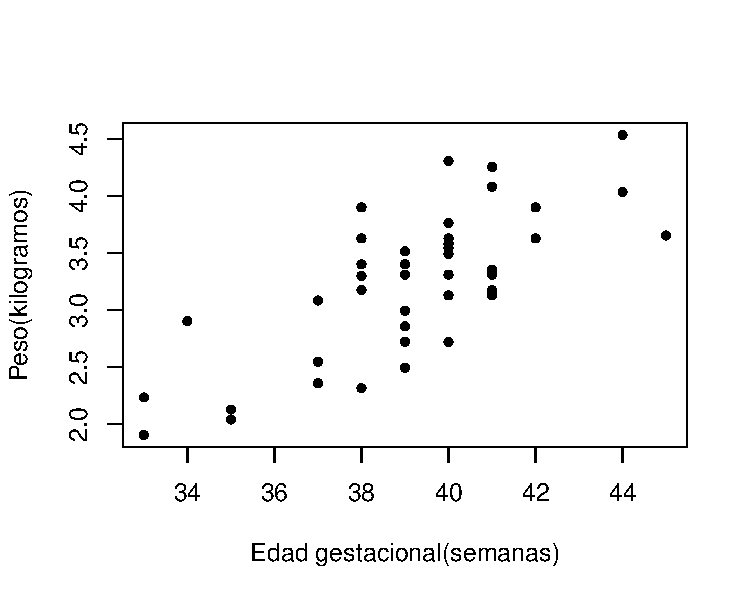
\includegraphics{MLG1_files/figure-latex/birthweightFigure-1} 

}

\caption{Gráfico de dispersion del peso del recien nacido y la edad gestacional.}\label{fig:birthweightFigure}
\end{figure}

Con este conjunto de datos podemos plantear las siguientes preguntas:

\begin{itemize}
\tightlist
\item
  ¿Cómo afecta la edad gestional al peso del neonato?
\item
  Si la edad gestacional aumenta en una unidad ¿en cuanto aumenta el peso del recién nacido? ¿ese aumento puede considerarse significativo?
\item
  ¿Se puede predecir el peso al nacer por medio de la edad gestacional?
\end{itemize}

Estas preguntas se pueden resolver a partir de un análisis de regresión lineal.

\hypertarget{regresion-lineal-simple}{%
\subsection{Regresion lineal simple}\label{regresion-lineal-simple}}

En un análisis de regresión simple estamos interesados en modelar la relación entre una variable de entrada (regresor, variable independiente o covariable) \(X\) y una variable de salida (respuesta o variable dependiente) \(Y\). Este modelo nos permite:

\begin{itemize}
\tightlist
\item
  Evaluar cuanto cambia el valor esperado de \(Y\) debido a cambios en \(X\),
\item
  Predecir \(Y\) (o su valor esperado) en función de \(X\).
\end{itemize}

\hypertarget{modelo-lineal-simple-1}{%
\subsection{Modelo lineal simple}\label{modelo-lineal-simple-1}}

Sea \((y_{i},x_{i})\) la i-ésima observación de la variable respuesta \((y)\) y la covariable \((x)\), para \(i=1,\ldots,n\), con \(n\) igual al número total de observaciones. \textbf{El modelo lineal simple} se puede expresar de la forma:
\[
y_{i} = \beta_{0} + x_{i}\beta_{1}+\varepsilon_{i},
\]
donde \(\beta_{0}\) es el intercepto, \(\beta_{1}\) es la pendiente y \(\varepsilon_{i}\) es el componente de error. Generalmente, los supuestos que acompañan este modelo son:

\begin{enumerate}
\def\labelenumi{\alph{enumi}.}
\tightlist
\item
  \(E(\varepsilon_{i}) = 0\),
\item
  \(V(\varepsilon_{i}) = \sigma^{2}\),
\item
  \(cov(\varepsilon_{i},\varepsilon_{j}) = 0\), para todo \(i \neq j\),
\item
  \(\varepsilon_{i}\) se distribuye normalmente.
\end{enumerate}

Por lo tanto, \(\varepsilon_{i} \sim N(0,\sigma^{2})\).

A partir de (a) se tiene que:
\[
E(Y|X=x_i) = \beta_{0} + x_i\beta_{1}.
\]
Entonces, para \(x=0\), el valor esperado de \(Y\) es igual a \(\beta_0\). Cuando \(X\) incrementa en una unidad (de \(x\) a \(x+1\)), el valor esperado de \(Y\) incrementa en:
\[
E(Y|X=x+1) - E(Y|X=x) = \beta_{0} + (x+1)\beta_{1} - (\beta_{0} + x\beta_{1}) = \beta_{1}.
\]
Lo que indica que \(\beta_{1}\) representa el cambio en el valor esperado de \(Y\) por un cambio unitario en \(X\).

Dado (b), tenemos que \(V(Y|X=x_{i}) = \sigma^{2}\). Es decir que para cualquier valor de \(x\), la varianza de \(Y\) es la misma (homocedasticidad). Puesto que los errores están incorrelacionados (c), entonces las observaciones de \(Y\) también lo están.

Debido a (d), tenemos que la variable respuesta se distribuye de forma normal. Específicamente, tenemos que: \(y_{i} \sim N(\beta_{0} + \beta_{1}x_i, \sigma^{2})\).

El proceso de generación de datos del modelo de regresión lineal se ilustra en la Figura \ref{fig:gendataFigure}. El valor esperado de \(Y|X\) está representado por la linea negra. Tenemos que, cada observación de \(y\) (puntos negros) es una realización de la distribución de \(Y|X=x_{i} \sim N(\beta_{0}+\beta_{1}x_{i},\sigma^{2})\) (curvas rojas). En esté ejemplo, suponemos que \(\beta_{0}=0\), \(\beta_{1}=1\), y \(\sigma=0.1\).

\begin{figure}

{\centering 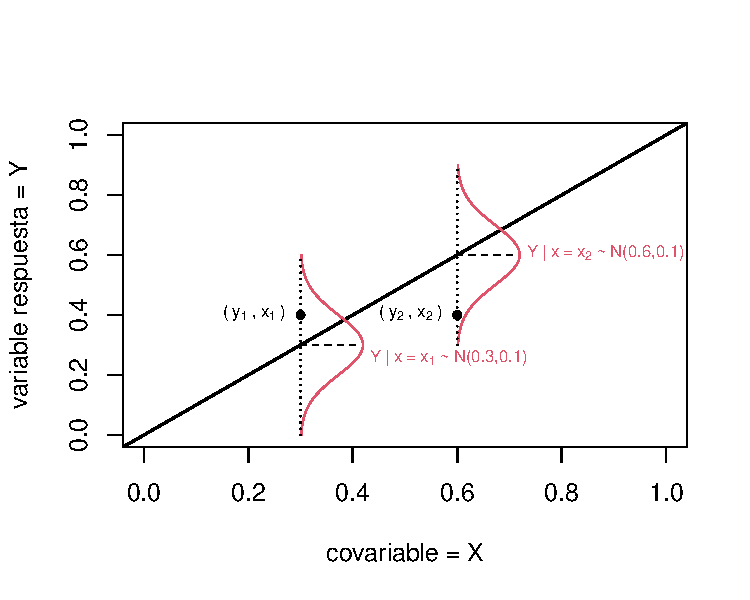
\includegraphics{MLG1_files/figure-latex/gendataFigure-1} 

}

\caption{Proceso generador datos del modelo lineal simple.}\label{fig:gendataFigure}
\end{figure}

\hypertarget{estimaciuxf3n-de-los-paruxe1metros}{%
\subsection{Estimación de los parámetros}\label{estimaciuxf3n-de-los-paruxe1metros}}

Los parámetros \(\beta_{0}\) y \(\beta_{1}\) son desconocidos y deben estimarse a partir de los datos. Para esto utilizamos el método de \textbf{mínimos cuadrados ordinarios (MCO)}.

La función objetivo es la siguiente:
\begin{equation}
S(\beta_{0},\beta_{1}) = \sum_{i=1}^{n} \left( y_{i} - \beta_{0} - \beta_{1}x_{i} \right)^{2} = \sum_{i=1}^{n} e_{i}^{2}.
 \label{eq:rss}
\end{equation}
Entonces, tenemos que encontrar la combinación de \(\beta_{0}\) y \(\beta_{1}\) que minimizan \eqref{eq:rss}. Para esto, primero debemos derivar \(S(\beta_{0},\beta_{1})\) con respecto a \(\beta_{0}\) y \(\beta_{1}\), e igualar estas ecuación a cero. De esta forma obtenemos las \textbf{ecuaciones normales}:
\begin{equation}
\frac{\partial S(\beta_{0},\beta_{1})}{\partial \beta_{0}} = - 2\sum_{i=1}^{n}\left(y_{i}-\beta_{0}-\beta_{1}x_{i} \right),
\label{eq:normeq1}
\end{equation}
y
\begin{equation}
\frac{\partial S(\beta_{0},\beta_{1})}{\partial \beta_{1}} = - 2\sum_{i=1}^{n}\left(y_{i}-\beta_{0}-\beta_{1}x_{i} \right)x_{i}.
\label{eq:normeq2}
\end{equation}

Los estimadores por MCO (\(\widehat{\beta}_{0}\) y \(\widehat{\beta}_{1}\)) se obtienen resolviendo el sistema de ecuaciones \eqref{eq:normeq1} y \eqref{eq:normeq2}:
\[
\widehat{\beta}_{0} = \bar{y} - \widehat{\beta}_{1}\bar{x},
\]
y
\[
\widehat{\beta}_{1} = \frac{\sum_{i=1}^{n}(x_{i}-\bar{x})(y_{i}-\bar{y})}{\sum_{i=1}^{n}(x_{i}-\bar{x})^2} = \frac{S_{xy}}{S_{xx}} =  cor(X,Y)\frac{s_{Y}}{s_{X}},
\]
donde \(s_{X}\) y \(s_{Y}\) son las desviaciones estándar muestrales de \(X\) y \(Y\).

La diferencia entre el valor observado \((y_{i})\) y el valor ajustado correspondiente \((\widehat{y}_{i})\) es llamado \textbf{residuo} (o residual):
\[
e_{i}= y_{i} - (\widehat{\beta}_{0} + \widehat{\beta}_{1}x_{i}) = y_{i}-\widehat{y}_{i}, \mbox{ para }i=1,\ldots,n.
\]
La Figura \ref{fig:Figresiduos} presenta los residuos de forma gráfica. Estos juegan un papel importante para la evaluar la bondad del ajuste del modelo (detectar posibles desviaciones a los supuestos asumidos).

\begin{figure}

{\centering 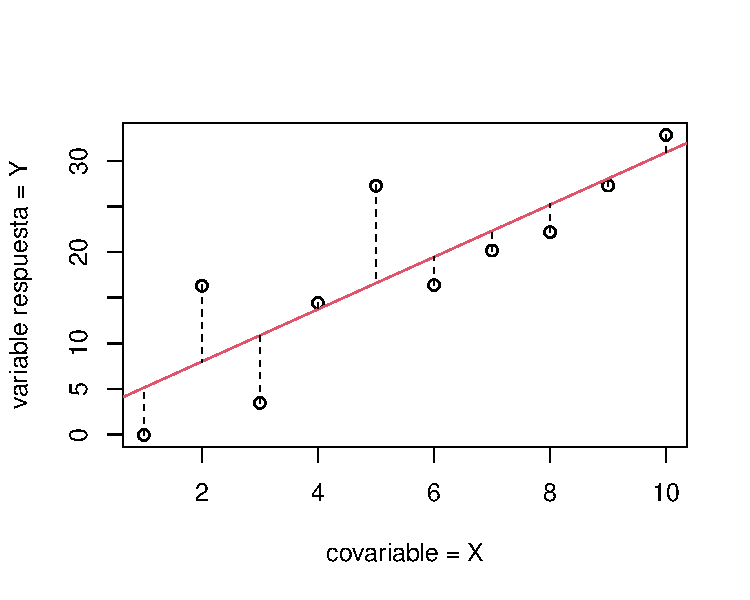
\includegraphics{MLG1_files/figure-latex/Figresiduos-1} 

}

\caption{Diagrama gráfico de un ajuste por MCO. La recta representa la estimación por MCO, y las lineas discontinuas verticales entre los puntos observados y la recta estimada son los residuos.}\label{fig:Figresiduos}
\end{figure}

\hypertarget{estimaciuxf3n-de-sigma2}{%
\subsection{\texorpdfstring{Estimación de \(\sigma^{2}\)}{Estimación de \textbackslash sigma\^{}\{2\}}}\label{estimaciuxf3n-de-sigma2}}

La estimación de \(\sigma^{2}\) se hace a partir de la suma de cuadrados de los residuos:
\[
SS_{res} = \sum_{i=1}^{n}e^{2}_{i} = \sum_{i=1}^{n} (y_{i}-\widehat{\beta}_{0} - \widehat{\beta}_{1}x_{i})^{2}.
\]
El valor esperado de \(SS_{res}\) es \(E(SS_{res})=(n-2)\sigma^{2}\) (Para el caso de regresión múltiple, ver Sección C.3 de \citet{montgomery_introduction_2012}). Por lo tanto, un estimador insesgado de \(\sigma^{2}\) es:
\[
\widehat{\sigma}^{2} = \frac{SS_{res}}{n-2} = MS_{res}.
\]
La cantidad \(MS_{res}\) es llamada \textbf{cuadrado medio de los residuos}.

\rule{\textwidth}{0.4pt}

\hypertarget{datos-de-peso-al-nacer.-modelo-y-estimaciuxf3n-de-parametros}{%
\subsubsection*{Datos de peso al nacer. Modelo y estimación de parametros}\label{datos-de-peso-al-nacer.-modelo-y-estimaciuxf3n-de-parametros}}
\addcontentsline{toc}{subsubsection}{Datos de peso al nacer. Modelo y estimación de parametros}

Para los datos de peso al nacer se propone el siguiente modelo:
\begin{equation}
\mbox{weight}_{i}= \beta_{0} + \beta_{1}\mbox{age}_{i} + \varepsilon_{i},
\label{eq:modBirthweight}
\end{equation}
donde \(\varepsilon_{i} \sim N(0,\sigma^{2})\).

En R, la estimación por MCO se realiza a través de la función \texttt{lm}:

\begin{Shaded}
\begin{Highlighting}[]
\NormalTok{mod }\OtherTok{=} \FunctionTok{lm}\NormalTok{(weight}\SpecialCharTok{\textasciitilde{}}\NormalTok{age, }\AttributeTok{data=}\NormalTok{birthweight)}
\NormalTok{mod}
\end{Highlighting}
\end{Shaded}

\begin{verbatim}
## 
## Call:
## lm(formula = weight ~ age, data = birthweight)
## 
## Coefficients:
## (Intercept)          age  
##     -3.6312       0.1752
\end{verbatim}

De aquí obtenemos que \(\widehat{\beta}_{0} =-3.63\) y \(\widehat{\beta}_{1} =0.18\). Note que la estimación del intercepto es negativa, lo que es físicamente imposible. Además tampoco tiene sentido una edad gestacional igual a cero. Por lo cual, este parámetro no tiene interpretación en este caso. \(\beta_{0}\) solo tiene interpretación cuando las observaciones de \(x\) están alrededor de cero.

A partir de \(\widehat{\beta}_{1}\), podemos concluir que la edad gestacional tiene un efecto positivo sobre el peso del recién nacido (el coeficiente estimado es positivo). Por cada incremento de una semana en la edad gestacional, el valor esperado del peso del recién nacido aumenta 0.18 kilogramos.

La representación gráfica del modelo estimado se presenta en la Figura \ref{fig:FigMCO2}.

\begin{Shaded}
\begin{Highlighting}[]
\FunctionTok{plot}\NormalTok{(weight}\SpecialCharTok{\textasciitilde{}}\NormalTok{age,}\AttributeTok{data=}\NormalTok{birthweight,}\AttributeTok{pch=}\DecValTok{20}\NormalTok{,}\AttributeTok{xlab=}\StringTok{"edad gestacional(semanas)"}\NormalTok{,}
     \AttributeTok{ylab=}\StringTok{\textquotesingle{}peso(kilogramos)\textquotesingle{}}\NormalTok{)}
\FunctionTok{abline}\NormalTok{(mod,}\AttributeTok{lwd=}\DecValTok{2}\NormalTok{)}
\end{Highlighting}
\end{Shaded}

\begin{figure}

{\centering 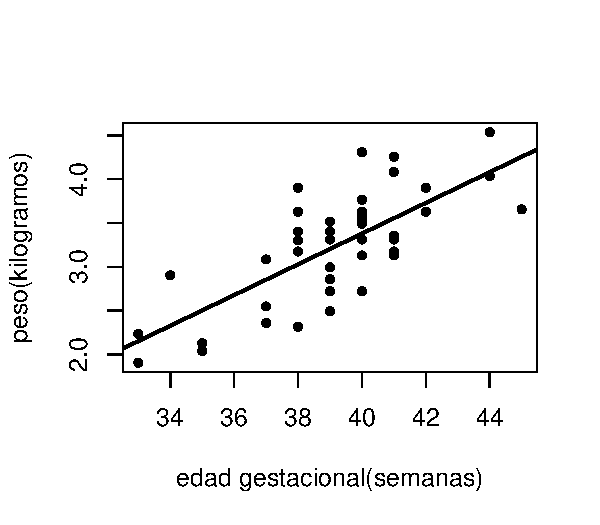
\includegraphics{MLG1_files/figure-latex/FigMCO2-1} 

}

\caption{Gráfico de dispersion del peso del recien nacido y la edad gestacional. La linea representa la estimación por MCO.}\label{fig:FigMCO2}
\end{figure}

La estimación de \(\sigma\) es:

\begin{Shaded}
\begin{Highlighting}[]
 \FunctionTok{sqrt}\NormalTok{(}\FunctionTok{sum}\NormalTok{(mod}\SpecialCharTok{$}\NormalTok{residuals}\SpecialCharTok{\^{}}\DecValTok{2}\NormalTok{)}\SpecialCharTok{/}\DecValTok{40}\NormalTok{)}
\end{Highlighting}
\end{Shaded}

\begin{verbatim}
## [1] 0.4376311
\end{verbatim}

\rule{\textwidth}{0.4pt}

\hypertarget{propiedades-de-los-estimadores-por-mco}{%
\subsection{Propiedades de los estimadores por MCO}\label{propiedades-de-los-estimadores-por-mco}}

Los estimadores de \(\widehat{\beta}_{0}\) y \(\widehat{\beta}_{1}\) son una combinación lineal de las observaciones:
\begin{equation}
\widehat{\beta}_{1} = \sum_{i=1}^{n} \frac{(x_{i}-\bar{x})(y_{i}-\bar{y})}{\sum_{i=1}^{n}(x_{i}-\bar{x})^2} = \sum_{i=1}^{n} \frac{(x_{i}-\bar{x})}{\sum_{i=1}^{n}(x_{i}-\bar{x})^2}y_{i} = \sum_{i=1}^{n}c_{i}y_{i}.
\label{eq:beta1cl}
\end{equation}
y
\[
\widehat{\beta}_{0} = \bar{y} - \widehat{\beta}_{1}\bar{x} = \sum_{i=1}^{n}\left( \frac{1}{n} - c_{i}\bar{x} \right)y_{i} = \sum_{i=1}^{n}d_{i}y_{i}.
\]
Además, se tiene que \(\sum_{i=1}^{n}c_{i}=0\) y \(\sum_{i=1}^{n}c_{i}x_{i}=1\). Los valores ajustados también son combinaciones lineales de los datos:
\[
\widehat{y}_{i} = \widehat{\beta}_{0} + \widehat{\beta}_{1}x_{i} = \sum_{i=1}^{n}(d_{i}+c_{i}x_{i})y_{i}.
\]
Puesto que los estimadores de \(\beta_{0}\) y \(\beta_{1}\) dependen de los errores, estos también son variables aleatorias. Por lo tanto debemos calcular el valor esperado y varianza de \(\widehat{\beta}_{0}\) y \(\widehat{\beta}_{1}\).

Si los supuestos del modelo se cumplen, tenemos que el valor esperado de \(\widehat{\beta}_{1}\) es:
\begin{equation}
\begin{split}
E(\widehat{\beta}_{1}) &= E\left( \sum_{i=1}^{n}c_{i}y_{i} \right) = \sum_{i=1}^{n}c_{i}E(y_{i}) = \sum_{i=1}^{n} c_{i}(\beta_{0} + \beta_{1}x_{i}) \\
&=\beta_{0}\sum_{i=1}^{n}c_{i} + \beta_{1}\sum_{i=1}^{n}c_{i}x_{i} = \beta_{1}.
\end{split}
\nonumber
\end{equation}
El valor esperado de \(\widehat{\beta}_{0}\) es:
\begin{equation}
\begin{split}
E(\widehat{\beta}_{0}) &= E\left(\bar{y} - \widehat{\beta}_{1}\bar{x} \right) = \frac{1}{n}\sum_{i=1}^{n}E(y_{i}) - \beta_{1}\bar{x} \\
&= \frac{1}{n}\sum_{i=1}^{n}\left(\beta_{0} + \beta_{1}x_{i}\right) - \beta_{1}\bar{x} = \beta_{0}.
\end{split}
\nonumber
\end{equation}

Es decir que \(\widehat{\beta}_{0}\) y \(\widehat{\beta}_{1}\) son estimadores insesgado de \(\beta_{0}\) y \(\beta_{1}\),respectivamente.

La varianza de \(\widehat{\beta}_{1}\) y \(\widehat{\beta}_{0}\) son:
\[
V(\widehat{\beta}_{1})= V \left( \sum_{i=1}^{n}c_{i}y_{i}\right) = \sum_{i=1}^{n}c_{i}^{2}V(y_{i}) = \sigma^{2}\sum_{i=1}^{n}c_{i}^{2} = \frac{\sigma^{2}}{S_{xx}},
\]
y
\begin{equation}
\begin{split}
V(\widehat{\beta}_{0}) &= V \left( \bar{y} - \widehat{\beta}_{1}\bar{x}\right) = V (\bar{y}) + \bar{x}^{2}V(\widehat{\beta}_{1}) - 2\bar{x}Cov(\bar{y},\widehat{\beta}_{1}) \\
&= \sigma^{2} \left(\frac{1}{n} + \frac{\bar{x}^{2}}{S_{xx}} \right),
\end{split}
\nonumber
\end{equation}
respectivamente. Finalmente, la covarianza entre \(\widehat{\beta}_{0}\) y \(\widehat{\beta}_{1}\) es:
\begin{equation}
\begin{split}
Cov(\widehat{\beta}_{0},\widehat{\beta}_{1}) &= Cov\left(\bar{y} - \widehat{\beta}_{1}\bar{x}, \widehat{\beta}_{1} \right) = Cov\left( \bar{y}, \widehat{\beta}_{1}\right) - \bar{x}V\left(\widehat{\beta}_{1}\right) \\
&=  - \sigma^{2}\frac{\bar{x}}{S_{xx}}.
\end{split}
\nonumber
\end{equation}

Si se cumple que \(E(\varepsilon_{i}) = 0\), \(V(\varepsilon_{i}) = \sigma^{2}\) y \(Cov(\varepsilon_{i},\varepsilon_{j})=0\), se puede probar que los estimadores por MCO son insesgado y de varianza mínima (\textbf{teorema de Gauss-Markov}). Para la demostración en el caso de regresión múltiple, ver Sección C4 de \citet{montgomery_introduction_2012}. Esto quiere decir que, comparado con todos los posibles estimadores insesgados que son combinación lineal de las observaciones, \(\widehat{\beta}_{0}\) y \(\widehat{\beta}_{1}\) tienen las varianzas más pequeñas. Por esto los estimadores por MCO son considerados los \textbf{mejores estimadores lineales insesgados}.

\hypertarget{inferencia}{%
\subsection{Inferencia}\label{inferencia}}

También podemos hacer pruebas de hipótesis e intervalos de confianza para los parámetros del modelo y/o pronósticos.

Por ejemplo, en los datos del peso al nacer podemos estar interesados en evaluar si la edad gestacional tiene un efecto positivo sobre el peso al nacer. Por lo tanto, debemos probar si \(\beta_{1} > 0\). También podríamos estar interesados en el valor esperado de un recién nacido para cierto valor especifico de edad gestacional, por ejemplo 38 semanas. Entonces, podemos calcular un intervalo de confianza para \(E(Y|x=38)\).

\hypertarget{pruebas-de-hipuxf3tesis}{%
\subsubsection{Pruebas de hipótesis}\label{pruebas-de-hipuxf3tesis}}

Suponga la siguiente hipótesis:
\begin{equation}
H_{0}: \beta_{1} = \beta_{10} \mbox{  } H_{1}: \beta_{1} \neq \beta_{10}.
\label{eq:H0beta1}
\end{equation}
Dado que \(\widehat{\beta}_{1}\) es una combinación lineal de \(y_{i}\) \eqref{eq:beta1cl}, podemos concluir que:
\[
\widehat{\beta}_{1} \sim N\left(\beta_{1}, \frac{\sigma^{2}}{S_{xx}}\right).
\]
Además,
\begin{equation}
t_{0} = \frac{\widehat{\beta}_{1}-\beta_{10}}{\sqrt{\frac{MS_{res}}{S_{xx}}}}\sim t_{n-2}.
\label{eq:distB1}
\end{equation}
Por lo tanto, \(t_{0}\) es el estadístico de prueba para las hipótesis \eqref{eq:H0beta1}. Entonces, rechazamos \(H_{0}\) si \(|t_{0}| \ge t_{1-\alpha/2,n-p}\) (o por medio del valor-\(p\) asociado).

De igual forma, para evaluar:
\[
H_{0}: \beta_{0} = \beta_{00} \mbox{  } H_{1}: \beta_{0} \neq \beta_{00},
\]
el estadístico de prueba es:
\begin{equation}
t_{0} = \frac{\widehat{\beta}_{0}-\beta_{00}}{\sqrt{MS_{res}\left(\frac{1}{n}+\frac{\bar{x}^{2}}{S_{xx}} \right)}} \sim t_{n-2}.
 \label{eq:distB0}
\end{equation}

\hypertarget{anuxe1lisis-de-varianza}{%
\subsubsection{Análisis de varianza}\label{anuxe1lisis-de-varianza}}

El análisis de varianza se basa en la partición de la variabilidad total de la variable respuesta \(y\) en dos componentes, uno debido al modelo ajustado y otro al error. Primero, empecemos con la siguiente identidad:
\begin{equation}
y_{i} - \bar{y} = (y_{i} - \widehat{y}_{i}) + (\widehat{y}_{i} - \bar{y}).
\label{eq:decomposion}
\end{equation}
La Figura \ref{fig:anovafig} muestra la partición \eqref{eq:decomposion} en el punto \(i=3\). Aquí vemos que una parte de la diferencia entre \(y_{3}\) y \(\bar{y}\) es explicada por el modelo (línea discontinua roja).

\begin{figure}

{\centering 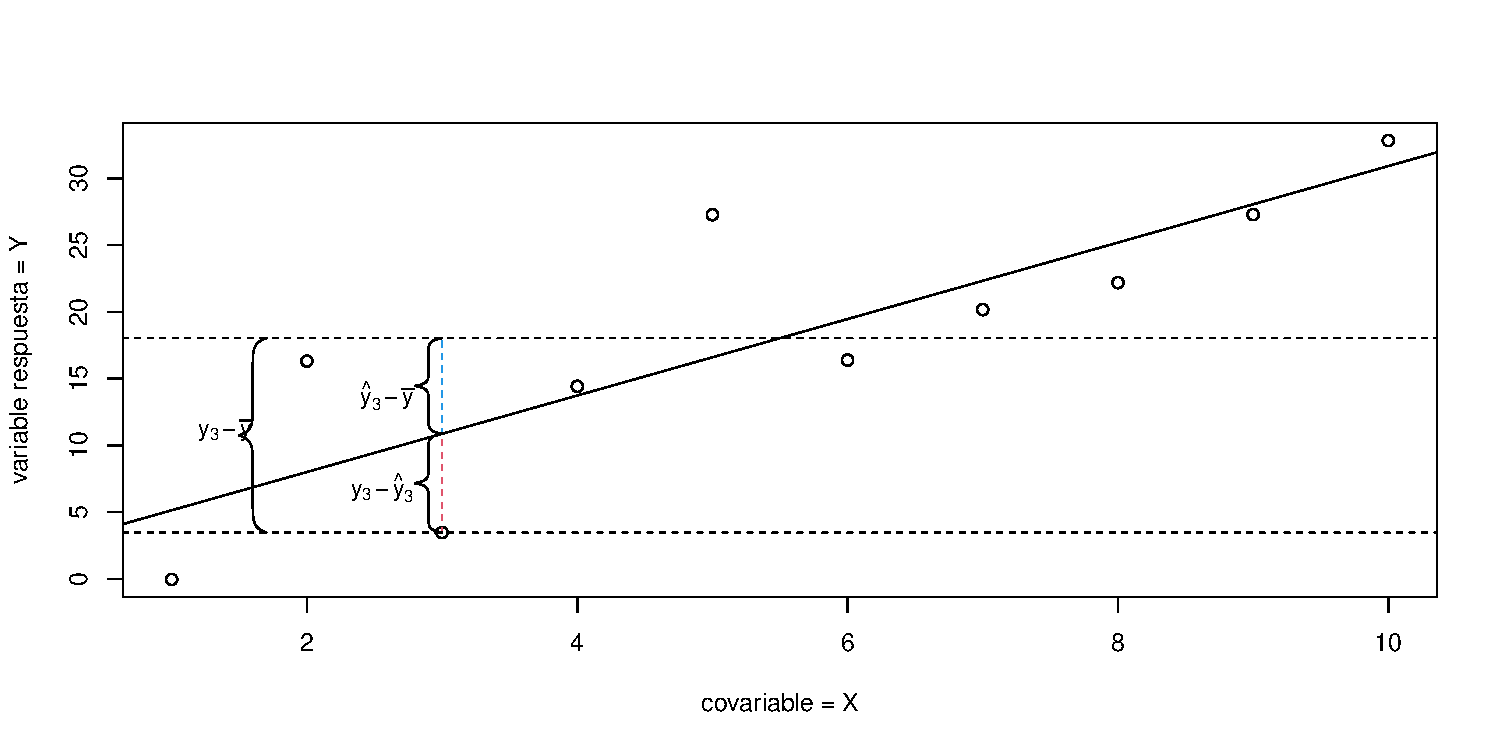
\includegraphics{MLG1_files/figure-latex/anovafig-1} 

}

\caption{Representación gráfica de la descompocisión \\eqref{eq:decomposion}.}\label{fig:anovafig}
\end{figure}

Ahora evelavamos al cuadrado \eqref{eq:decomposion} y sumamos todos los componentes:
\begin{equation}
\begin{split}
SSY &= \sum_{i=1}^{n} (y_{i} - \bar{y})^{2} \\
&= \sum_{i=1}^{n} (y_{i} - \widehat{y}_{i})^{2} + \sum_{i=1}^{n}(\widehat{y}_{i} - \bar{y})^{2} + 2 \sum_{i=1}^{n}(y_{i} - \widehat{y}_{i})(\widehat{y}_{i} - \bar{y}) \\
&= \sum_{i=1}^{n} (y_{i} - \widehat{y}_{i})^{2} + \sum_{i=1}^{n}(\widehat{y}_{i} - \bar{y})^{2} \\
SST &=  SS_{res} + SS_{R},
\end{split}
\label{eq:ss}
\end{equation}
donde \(SST\) es llamada la \textbf{suma de cuadrados totales} (con \(n-1\) grados de libertad), \(SS_{R}\) es la \textbf{suma de cuadrados de la regresión} (con \(1\) grados de libertad), y \(SS_{res}\) es la \textbf{suma de cuadrados residual o del error} (con \(n-2\) grados de libertad).

El análisis de varianza nos permite evaluar la siguiente hipótesis:
\begin{equation}
H_{0}: \beta_{1} = 0 \mbox{  }H_{1}:  \beta_{1} \neq 0.
\label{eq:anova}
\end{equation}

Se puede demostrar que si \(H_{0}\) es cierta:
\[
\frac{SS_{res}}{\sigma^{2}} = \frac{(n-2)MS_{res}}{\sigma^{2}} \sim \chi^{2}_{n-2} \mbox{,} \ \  \frac{SS_{R}}{\sigma^{2}} \sim \chi^{2}_{1},
\]
y que \(SS_{res}\) y \(SS_{R}\) son independientes. Por lo tanto:
\[
F_{0} = \frac{SS_{R}/1}{SS_{res}/(n-2)} = \frac{MS_{R}}{MS_{res}} \sim F_{(1,n-2)}.
\]
Además, \(E(MS_{res})=\sigma^{2}\) y \(E(MS_{R})=\sigma^{2} + \beta_{1}^{2}S_{xx}\).

Entonces, podemos utilizar \(F_{0}\) como estadístico de prueba de \eqref{eq:anova}. Rechazamos \(H_{0}\) si \(F_{0} > F_{\alpha,1,n-2}\).

Si \(H_{0}\) es falsa, \(F_{0}\) sigue una distribución F no central con \(1\) y \(n-2\) grados de libertad, y parámetro de no centralidad igual a \(\lambda=(\beta_{1}^{2}S_{xx})/\sigma^{2}\).

Estos resultados se pueden resumir en la Tabla \ref{tab:tableAnova}.

\begin{longtable}[]{@{}rrrrr@{}}
\caption{\label{tab:tableAnova} Tabla de ANOVA}\tabularnewline
\toprule\noalign{}
Fuente de variación & g.l. & SS & MS & \(F\) \\
\midrule\noalign{}
\endfirsthead
\toprule\noalign{}
Fuente de variación & g.l. & SS & MS & \(F\) \\
\midrule\noalign{}
\endhead
\bottomrule\noalign{}
\endlastfoot
regresión & 1 & \(SS_{R}\) & \(MS_{R}\) & \(F_{0}\) \\
residuos & n-2 & \(SS_{res}\) & \(MS_{res}\) & \\
Total & n-1 & \(SST\) & & \\
\end{longtable}

La cantidad:
\[
R^{2} = \frac{SS_{R}}{SST} = 1 - \frac{SS_{res}}{SST},
\]
es llamada \textbf{coeficiente de determinación}, y cuantifica la cantidad de variabilidad de \(y\) que es explicada por \(x\). Dado que \(0 \leq SS_{res} \leq SST\), se tiene que \(0 \leq R^{2} \leq 1\). Por lo tanto, valores cercanos a \(1\) implican que el modelo explica gran parte de la variabilidad de \(y\).

\rule{\textwidth}{0.4pt}

\hypertarget{datos-de-peso-al-nacer.-pruebas-de-hipuxf3tesis-y-anova}{%
\subsubsection*{Datos de peso al nacer. Pruebas de hipótesis y ANOVA}\label{datos-de-peso-al-nacer.-pruebas-de-hipuxf3tesis-y-anova}}
\addcontentsline{toc}{subsubsection}{Datos de peso al nacer. Pruebas de hipótesis y ANOVA}

Se quiere probar que la edad gestacional tiene influencia sobre el peso al nacer del recién nacido. Esto es:
\[
H_{0}: \beta_{1} = 0 \qquad H_{1}: \beta_{1} \neq 0. 
\]
Tanto la prueba de hipótesis basada en \(t_{0}\), el valor \(F_{0}\) del ANOVA, y el \(R^{2}\) se pueden observar usando la función \texttt{summary}:

\begin{Shaded}
\begin{Highlighting}[]
\FunctionTok{summary}\NormalTok{(mod)}
\end{Highlighting}
\end{Shaded}

\begin{verbatim}
## 
## Call:
## lm(formula = weight ~ age, data = birthweight)
## 
## Residuals:
##      Min       1Q   Median       3Q      Max 
## -0.71314 -0.36708  0.01982  0.26741  0.93034 
## 
## Coefficients:
##             Estimate Std. Error t value Pr(>|t|)    
## (Intercept) -3.63119    1.01556  -3.576 0.000932 ***
## age          0.17525    0.02586   6.778 3.83e-08 ***
## ---
## Signif. codes:  0 '***' 0.001 '**' 0.01 '*' 0.05 '.' 0.1 ' ' 1
## 
## Residual standard error: 0.4376 on 40 degrees of freedom
## Multiple R-squared:  0.5346, Adjusted R-squared:  0.5229 
## F-statistic: 45.94 on 1 and 40 DF,  p-value: 3.828e-08
\end{verbatim}

Del resultado anterior, tenemos que:

\begin{itemize}
\tightlist
\item
  \(t_{0}=6.778\) con un valor-\(p\) asociado de 0. Por lo tanto, rechazamos \(H_{0}\) y concluimos que la edad gestacional tiene un efecto significativo sobre el peso al nacer.
\item
  La función \texttt{summary} no arroja como resultado una tabla ANOVA. Pero podemos observar el valor \(F_{0} = 45.94\) con un valor \(p\) asociado de 0.
\item
  \(R^{2} = 0.535\), lo que indica que el 53.5\% de la variabilidad del peso al nacer es explicada por la edad gestacional.

  \rule{\textwidth}{0.4pt}
\end{itemize}

\hypertarget{intervalos-de-confianza}{%
\subsubsection{Intervalos de confianza}\label{intervalos-de-confianza}}

\hypertarget{intervalos-de-confianza-para-beta_0-beta_1-y-sigma2}{%
\paragraph*{\texorpdfstring{Intervalos de confianza para \(\beta_{0}\), \(\beta_{1}\) y \(\sigma^{2}\)}{Intervalos de confianza para \textbackslash beta\_\{0\}, \textbackslash beta\_\{1\} y \textbackslash sigma\^{}\{2\}}}\label{intervalos-de-confianza-para-beta_0-beta_1-y-sigma2}}
\addcontentsline{toc}{paragraph}{Intervalos de confianza para \(\beta_{0}\), \(\beta_{1}\) y \(\sigma^{2}\)}

Los intervalos de confianza para \(\beta_{0}\) y \(\beta_{1}\) se construyen a partir de las distribuciones de probabilidad de \(\widehat{\beta}_{0}\) y \(\widehat{\beta}_{1}\). Esto es, \eqref{eq:distB0} y \eqref{eq:distB1}, respectivamente.

Por lo tanto, el intervalo del \(100(1-\alpha)\%\) de confianza para \(\beta_{j}\) es:
\[
\widehat{\beta}_{j} \pm t_{1-\alpha/2,n-2}\sqrt{V(\widehat{\beta}_{j})}, \mbox{ para }j=0,1.
\]
Se puede demostrar que \((n-2)MS_{res}/\sigma^{2}\sim \chi^{2}_{n-2}\). Por lo tanto:
\[
P \left\{ \chi^{2}_{\alpha/2,n-2} \leq (n-2)MS_{res}/\sigma^{2} \leq \chi^{2}_{1-\alpha/2,n-2} \right\} = 1-\alpha.
\]
Entonces, el intervalo del \(100(1-\alpha)\%\) de confianza para \(\sigma^{2}\) es:
\[
\left\{ \frac{(n-2)MS_{res}}{\chi^{2}_{1-\alpha/2,n-2}}; \frac{(n-2)MS_{res}}{\chi^{2}_{\alpha/2,n-2}} \right\}.
\]

\hypertarget{intervalos-de-confianza-para-ey_i-y-una-predicciuxf3n-futura}{%
\paragraph*{\texorpdfstring{Intervalos de confianza para \(E(y_{i})\) y una predicción futura}{Intervalos de confianza para E(y\_\{i\}) y una predicción futura}}\label{intervalos-de-confianza-para-ey_i-y-una-predicciuxf3n-futura}}
\addcontentsline{toc}{paragraph}{Intervalos de confianza para \(E(y_{i})\) y una predicción futura}

Cuando el objetivo de ajustar un modelo de regresión es hacer predicciones, es posible hacer intervalos de confianza para la respuesta media, esto es \(E(Y|x_{0})=\mu_{Y|x_{0}}\), donde \(x_{0}\) es un valor de la covariable dentro del rango de valores observados de \(x\) en los datos.

Una estimación insesgada de \(\mu_{Y|x_{0}}\) es:
\[
\widehat{\mu}_{Y|x_{0}} = \widehat{\beta}_{0} + \widehat{\beta}_{1}x_{0}.
\]
La varianza de \(\widehat{\mu}_{Y|x_{0}}\) es:
\begin{equation}
\begin{split}
V(\widehat{\mu}_{Y|x_{0}}) &= V(\widehat{\beta}_{0} + \widehat{\beta}_{1}x_{0}) = V(\widehat{\beta}_{0}) + x_{0}^{2}V(\widehat{\beta}_{1}) + 2x_{0}Cov(\widehat{\beta}_{0},\widehat{\beta}_{1}) \\
&= \sigma^{2}\left(\frac{1}{n} + \frac{\bar{x}^{2}}{S_{xx}} \right) + \sigma^{2}x_{0}^{2}\frac{1}{S_{xx}} - 2\sigma^{2}x_{0}\frac{\bar{x}}{S_{xx}} \\
&= \sigma^{2}\left[\frac{1}{n} + \frac{(x_{0}-\bar{x})^{2}}{S_{xx}} \right].
\end{split}
\nonumber
\end{equation}
El intervalo de confianza se construye a partir de la siguiente distribución muestral:
\[
\frac{\widehat{\mu}_{Y|x_{0}} - E(Y|x_{0})}{\sqrt{MS_{res}[1/n+(x_{0}-\bar{x})^{2}/S_{xx}]}} \sim t_{n-2}.
\]
Por lo tanto, el intervalo del \(100(1-\alpha)\%\) de confianza para \(\mu_{Y|x_{0}}\) es:
\begin{equation}
\widehat{\mu}_{Y|x_{0}} \pm t_{1-\alpha/2,n-2}\sqrt{MS_{res}[1/n+(x_{0}-\bar{x})^{2}/S_{xx}]}.
\label{eq:CImean}
\end{equation}
Note que la longitud del intervalo de confianza de \(\widehat{\mu}_{Y|x_{0}}\) depende del punto \(x_{0}\). La menor longitud se obtiene en el punto \(x_{0}=\bar{x}\), y el intervalo es cada vez mas ancho a medida que nos alejamos de ese punto.

Ahora consideremos hacer una predicción de una observación futura de \(y\) para cierto valor de \(x\). Si queremos hacer la predicción para \(x=x_{0}\), entonces la predicción de la nueva observación es:
\[
\widetilde{y}_{0} = \widehat{\beta}_{0} + \widehat{\beta}_{1}x_{0}.
\]
Asumiendo que el modelo es correcta, el verdadero valor de \(y_{0}\) es:
\[
\widetilde{y}_{0} = \widehat{\beta}_{0} + \widehat{\beta}_{1}x_{0} + \varepsilon_{0}.
\]
y su varianza es:
\begin{equation}
V(\widetilde{y}_{0}) = \sigma^{2}+\sigma^{2}\left[\frac{1}{n} + \frac{(x_{0}-\bar{x})^{2}}{S_{xx}} \right].
\label{eq:varpred}
\end{equation}
El primer término a la derecha de \eqref{eq:varpred} corresponde a la variabilidad de \(\varepsilon_{0}\) y el segundo al error de estimación de los coeficientes \(\beta_{0}\) y \(\beta_{1}\). A partir de estos resultados, el intervalo del \(100(1-\alpha)\%\) de predicción de una observación futura en \(x=x_{0}\) es:
\[
\widehat{\mu}_{Y|x_{0}} \pm t_{1-\alpha/2,n-2}\sqrt{MS_{res}[1+1/n+(x_{0}-\bar{x})^{2}/S_{xx}]}.
\]

\rule{\textwidth}{0.4pt}

\hypertarget{datos-de-peso-al-nacer.-intervalos-de-confianza}{%
\subsubsection*{Datos de peso al nacer. Intervalos de confianza}\label{datos-de-peso-al-nacer.-intervalos-de-confianza}}
\addcontentsline{toc}{subsubsection}{Datos de peso al nacer. Intervalos de confianza}

El intervalo del 95\% de confianza para los parámetros del modelo \eqref{eq:modBirthweight} son:

\begin{Shaded}
\begin{Highlighting}[]
\FunctionTok{confint}\NormalTok{(mod)}
\end{Highlighting}
\end{Shaded}

\begin{verbatim}
##                  2.5 %     97.5 %
## (Intercept) -5.6837190 -1.5786621
## age          0.1229923  0.2275067
\end{verbatim}

Para \(\beta_{1}\), con un nivel de confianza del 95\% podemos decir que cuando la edad gestacional aumenta en una unidad, el peso medio del recién nacido aumenta entre 123 y 228 gramos. Como mencionamos antes, \(\beta_{0}\) no tiene interpretación en este modelo.

El intervalo del 95\% de confianza para \(\sigma\) se calcula ``a pie'' de la siguiente forma:

\begin{Shaded}
\begin{Highlighting}[]
\NormalTok{var.limInf }\OtherTok{=} \FunctionTok{sum}\NormalTok{(mod}\SpecialCharTok{$}\NormalTok{residuals}\SpecialCharTok{\^{}}\DecValTok{2}\NormalTok{)}\SpecialCharTok{/}\FunctionTok{qchisq}\NormalTok{(}\FloatTok{0.975}\NormalTok{,}\AttributeTok{df=}\NormalTok{mod}\SpecialCharTok{$}\NormalTok{df.residual)}
\NormalTok{var.limSup }\OtherTok{=} \FunctionTok{sum}\NormalTok{(mod}\SpecialCharTok{$}\NormalTok{residuals}\SpecialCharTok{\^{}}\DecValTok{2}\NormalTok{)}\SpecialCharTok{/}\FunctionTok{qchisq}\NormalTok{(}\FloatTok{0.025}\NormalTok{,}\AttributeTok{df=}\NormalTok{mod}\SpecialCharTok{$}\NormalTok{df.residual)}
\FunctionTok{sqrt}\NormalTok{(}\FunctionTok{c}\NormalTok{(var.limInf,var.limSup))}
\end{Highlighting}
\end{Shaded}

\begin{verbatim}
## [1] 0.3593008 0.5599503
\end{verbatim}

Se quiere predecir el peso medio de los recién nacidos en la semana gestacional 36. La estimación puntual es:
\[
\widehat{\mu}_{Y|x_{0}=36} = \widehat{\beta}_{0} + \widehat{\beta}_{1}(36) = -3.6312 + 0.1751*36 = 2.672.
\]
El intervalo del 95\% de confianza para \(\widehat{\mu}_{Y|x_{0}=36}\) se puede calcular de la siguiente forma:

\begin{Shaded}
\begin{Highlighting}[]
\NormalTok{x.nuevo }\OtherTok{=} \FunctionTok{data.frame}\NormalTok{(}\AttributeTok{age=}\DecValTok{36}\NormalTok{)}
\NormalTok{pred.media }\OtherTok{=} \FunctionTok{predict}\NormalTok{(mod,x.nuevo,}\AttributeTok{interval =} \StringTok{\textquotesingle{}confidence\textquotesingle{}}\NormalTok{)}
\NormalTok{pred.media}
\end{Highlighting}
\end{Shaded}

\begin{verbatim}
##        fit     lwr      upr
## 1 2.677792 2.46233 2.893254
\end{verbatim}

Esto quiere decir que, con un nivel de confianza del 95\%, el peso medio de los recién nacidos en la semana gestacional 36 está entre 2.46 y 2.89 kilogramos.

Ahora, se quiere predecir el peso de un recién nacido en la semana gestacional 38, para esto calculamos un intervalo de predicción del 95\%:

\begin{Shaded}
\begin{Highlighting}[]
\NormalTok{x.nuevo }\OtherTok{=} \FunctionTok{data.frame}\NormalTok{(}\AttributeTok{age=}\DecValTok{38}\NormalTok{)}
\NormalTok{pred.nuevaObs }\OtherTok{=} \FunctionTok{predict}\NormalTok{(mod,x.nuevo,}\AttributeTok{interval =} \StringTok{\textquotesingle{}prediction\textquotesingle{}}\NormalTok{)}
\NormalTok{pred.nuevaObs}
\end{Highlighting}
\end{Shaded}

\begin{verbatim}
##        fit      lwr      upr
## 1 3.028291 2.131178 3.925404
\end{verbatim}

Por lo tanto, con un nivel de confianza del 95\% el peso de un recién nacido en la semana gestacional 38 está entre 2.13 y 3.93 kilogramos.

Gráficamente, podemos ver los intervalos de confianza y predicción de la siguiente forma. Primero hacemos la predicciones para edades gestacionales entre 33 y 45 semanas:

\begin{Shaded}
\begin{Highlighting}[]
\NormalTok{x.nuevo }\OtherTok{=} \FunctionTok{data.frame}\NormalTok{(}\AttributeTok{age=}\FunctionTok{seq}\NormalTok{(}\AttributeTok{from=}\DecValTok{33}\NormalTok{,}\AttributeTok{to=}\DecValTok{45}\NormalTok{,}\AttributeTok{length.out =} \DecValTok{100}\NormalTok{))}
\NormalTok{pred.media }\OtherTok{=} \FunctionTok{predict}\NormalTok{(mod,x.nuevo,}\AttributeTok{interval =} \StringTok{\textquotesingle{}confidence\textquotesingle{}}\NormalTok{)}
\NormalTok{pred.nuevaObs }\OtherTok{=} \FunctionTok{predict}\NormalTok{(mod,x.nuevo,}\AttributeTok{interval =} \StringTok{\textquotesingle{}prediction\textquotesingle{}}\NormalTok{)}
\end{Highlighting}
\end{Shaded}

Luego hacemos el gráfico:

\begin{Shaded}
\begin{Highlighting}[]
\FunctionTok{plot}\NormalTok{(weight}\SpecialCharTok{\textasciitilde{}}\NormalTok{age,}\AttributeTok{data=}\NormalTok{birthweight,}\AttributeTok{pch=}\DecValTok{20}\NormalTok{,}\AttributeTok{xlab=}\StringTok{"Edad gestacional(semanas)"}\NormalTok{,}
     \AttributeTok{ylab=}\StringTok{\textquotesingle{}Peso(kilogramos)\textquotesingle{}}\NormalTok{)}
\FunctionTok{abline}\NormalTok{(mod)}
\FunctionTok{lines}\NormalTok{(x.nuevo}\SpecialCharTok{$}\NormalTok{age,pred.media[,}\DecValTok{2}\NormalTok{],}\AttributeTok{lty=}\DecValTok{2}\NormalTok{)}
\FunctionTok{lines}\NormalTok{(x.nuevo}\SpecialCharTok{$}\NormalTok{age,pred.media[,}\DecValTok{3}\NormalTok{],}\AttributeTok{lty=}\DecValTok{2}\NormalTok{)}
\FunctionTok{lines}\NormalTok{(x.nuevo}\SpecialCharTok{$}\NormalTok{age,pred.nuevaObs[,}\DecValTok{2}\NormalTok{],}\AttributeTok{lty=}\DecValTok{3}\NormalTok{)}
\FunctionTok{lines}\NormalTok{(x.nuevo}\SpecialCharTok{$}\NormalTok{age,pred.nuevaObs[,}\DecValTok{3}\NormalTok{],}\AttributeTok{lty=}\DecValTok{3}\NormalTok{)}
\end{Highlighting}
\end{Shaded}

\begin{figure}

{\centering 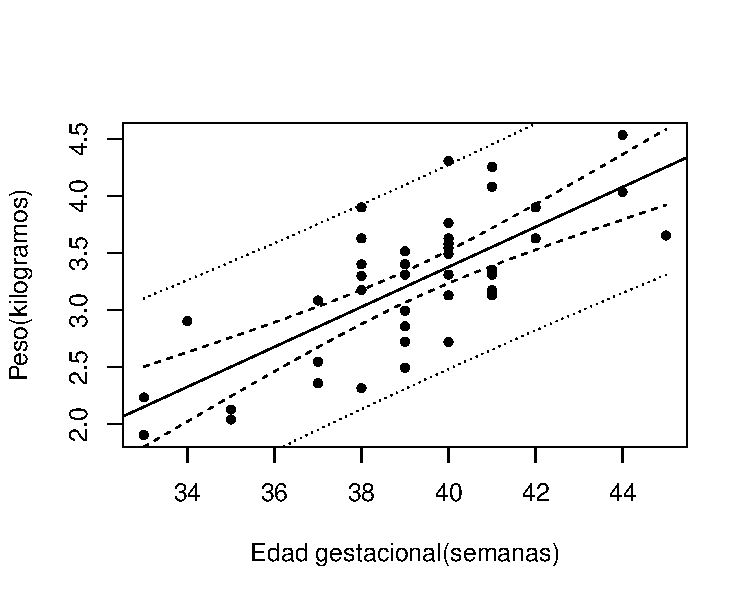
\includegraphics{MLG1_files/figure-latex/birthweightIC-1} 

}

\caption{\label{fig:BWdata2} Intervalos del 95\% de confianza (línea discontinua) y predicción (línea punteada) para el peso del recien nacido en función de la edad gestacional.}\label{fig:birthweightIC}
\end{figure}
\rule{\textwidth}{0.4pt}

\hypertarget{estimador-por-muxe1xima-verosimilitud}{%
\subsection{Estimador por máxima verosimilitud}\label{estimador-por-muxe1xima-verosimilitud}}

Si consideramos que \(\varepsilon_{i}\sim N(0,\sigma^{2})\), entonces las observación también se distribuyen de forma normal \(y_{i}\sim N(\beta_{0}+\beta_{1}x_{i},\sigma^{2})\). Si además asumimos que las observaciones \((y_{i},x_{i})\) son independientes, entonces la función de verosimilitud es:
\begin{equation}
\begin{split}
L(\boldsymbol \theta) =& \prod_{i=1}^{n} \left(\sqrt{2\pi\sigma^{2}} \right)^{-1/2}\exp\left[ - \frac{1}{2\sigma^{2}}(y_{i}-\beta_{0}-\beta_{1}x_{i})^{2} \right] \\
=& \left( \sqrt{2\pi\sigma^{2}} \right)^{-n/2}\exp\left[ - \frac{1}{2\sigma^{2}} \sum_{i=1}^{n}(y_{i}-\beta_{0}-\beta_{1}x_{i})^{2}\right],
\end{split}
\nonumber
\end{equation}
para \(\boldsymbol \theta=(\beta_{0},\beta_{1},\sigma^{2})'\). La log-verosimilitud es:
\[
\ell (\boldsymbol \theta) = - \left(\frac{n}{2}\right)\left[ \log (2 \pi) - \log \sigma^{2}\right] - \frac{1}{2\sigma^{2}}\sum_{i=1}^{n}(y_{i} - \beta_{0}-\beta_{1}x_{i})^{2}. 
\]
El estimador de máxima verosimilitud de \(\boldsymbol \theta\) debe satisfacer:
\[
\left. \frac{\partial \ell(\boldsymbol \theta)}{\partial \beta_{0}} \right|_{\widetilde{\boldsymbol \theta}} = \frac{1}{\widetilde{\sigma}^{2}}\sum_{i=1}^{n}(y_{i} - \beta_{0}-\beta_{1}x_{i}) = 0,
\]
\[
\left. \frac{\partial \ell(\boldsymbol \theta)}{\partial \beta_{1}} \right|_{\widetilde{\boldsymbol \theta}} = \frac{1}{\widetilde{\sigma}^{2}}\sum_{i=1}^{n}(y_{i} - \beta_{0}-\beta_{1}x_{i})x_{i} = 0,
\]
y
\[
\left. \frac{\partial \ell(\boldsymbol \theta)}{\partial \sigma^{2}} \right|_{\widetilde{\boldsymbol \theta}} = -\frac{n}{2\widetilde{\sigma}^{2}} + \frac{n}{2\widetilde{\sigma}^{4}}
\sum_{i=1}^{n}(y_{i} - \beta_{0}-\beta_{1}x_{i})^{2} = 0,
\]
Luego de solucionar las ecuaciones anteriores se obtienen los estimadores por máxima verosimilitud:
\[
\widetilde{\beta}_{0} = \bar{y} - \widetilde{\beta}_{1}\bar{x},
\]
\[
\widetilde{\beta}_{1} = \frac{\sum_{i=1}^{n}y_{i}(x_{i}-\bar{x})}{\sum_{i=1}^{n}(x_{i}-\bar{x})^{2}},
\]
y
\[
\widetilde{\sigma}^{2} = \frac{\sum_{i=1}^{n}(y_{i}-\beta_{0}-\beta_{1}x_{i})^{2}}{n}.
\]
Aquí observamos que los estimadores por máxima verosimilitud para \(\beta_{0}\) y \(\beta_{1}\) son equivalente a los estimadores por MCO. El estimador de \(\sigma^{2}\) es sesgado, sin embargo el sesgo disminuye a medida que \(n\) crece.

Por lo general, los estimadores por máxima verosimilitud tienen mejores propiedades que los estimadores por MCO. Son asintoticamente insesgados, consistentes y asintoticamente de mínima varianza. Sin embargo, estos requieren de supuestos distribucionales completos. Recordemos que los estimadores por MCO solo requieren de una correcta especificación de los dos primeros momentos (valor esperado, varianza y covarianza).

\hypertarget{algunas-consideraciones-finales}{%
\subsection{Algunas consideraciones finales}\label{algunas-consideraciones-finales}}

\begin{itemize}
\tightlist
\item
  Las conclusiones sobre los modelos de regresión se hacen sobre el rango de valores observados de las covariables (interpolación). Por ejemplo, en los datos de los recién nacidos, se pueden hacer inferencias sobre el peso al nacer para bebés que nacen en entre las semanas 33 y 45. Cuando hacemos predicciones fuera de este rango estaríamos extrapolando.
\end{itemize}

Por extrapolación nos referimos a hacer predicciones fuera del rango observado de \(x\). La Figura \ref{fig:extrapolacion} muestra el problema que se puede cometer cuando extrapolamos. Si tenemos datos en el rango \(x_{min} \leq x \leq x_{max}\), un modelo lineal es una buena aproximación de \(E(Y|x)\). Pero, esa aproximación no es buena para \(x>x_{max}\). Por lo tanto, se estaría cometiendo errores graves cuando hacemos predicciones de \(Y\) para valores de \(x\) mayores a \(x_{max}\) (por ejemplo en el punto \(x_{0}\)).

\begin{figure}

{\centering 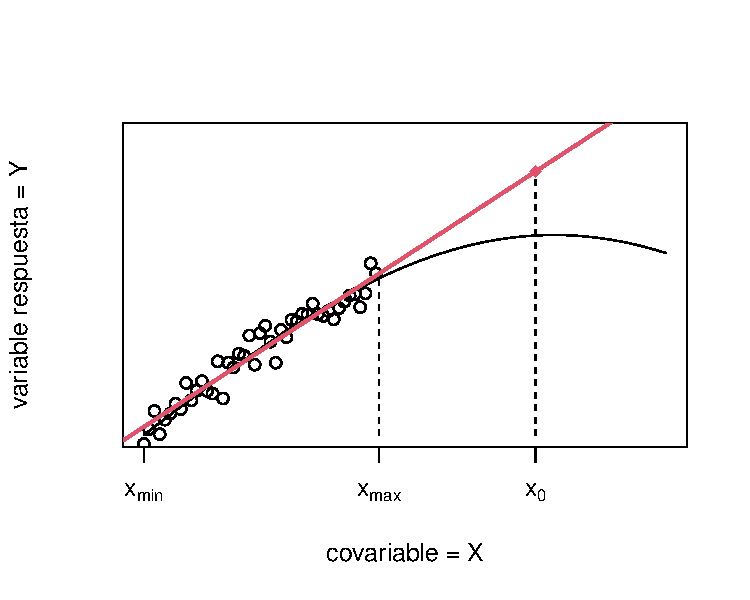
\includegraphics{MLG1_files/figure-latex/extrapolacion-1} 

}

\caption{Peligro de extrapolar. La curva negra representa $E(Y|x)$ y la línea roja es el ajuste del modelo lineal con los datos observados de $x$. La predicción en el punto $x_{0}$ es bastante sesgada.}\label{fig:extrapolacion}
\end{figure}

\begin{itemize}
\item
  La posición de los valores de \(x\) tienen una influencia sobre el ajuste por MCO. Particularmente, la estimación de \(\beta_{1}\) está fuertemente influenciada por los valores alejados de \(x\) y \(y\). A estos puntos se les denomina \textbf{puntos influyentes}. En la Figura \ref{fig:influyentes}(a) podemos ver como un solo punto tiene una influencia alta en la estimación de los parámetros del modelo.
\item
  Los \textbf{valores atípicos} son observaciones que difieren considerablemente del resto de los datos (generalmente en \(y\)). Un punto atípico puede afectar la estimación de \(\beta_{0}\) (ver Figura \ref{fig:influyentes}(b) y la estimación de \(\sigma^{2}\).
\end{itemize}

\begin{figure}

{\centering 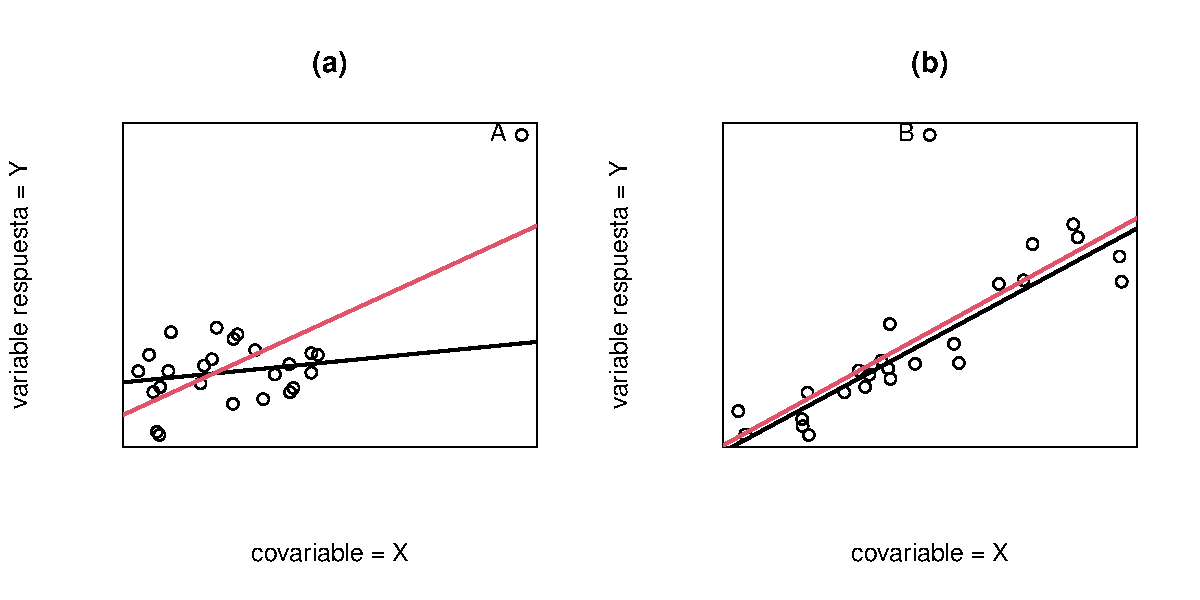
\includegraphics{MLG1_files/figure-latex/influyentes-1} 

}

\caption{(a) Efecto de un punto influyente, la línea negra  es la estimación sin el punto A y la linea roja es la estimación incluyento el punto A. (b) Efecto de un punto atípico, la línea negra  es la estimación sin el punto B y la linea roja es la estimación incluyento el punto B.}\label{fig:influyentes}
\end{figure}

Los métodos para la detección de puntos atípicos e influyentes se presentarán en un capítulo posterior.

\begin{itemize}
\tightlist
\item
  Una fuerte relación entre dos variables no necesariamente implica que la relación entre las variables es de causa-efecto. Un modelo de regresión nos permite modelar variables que estén correlacionadas, pero no se puede concluir que, necesariamente, es una relación causal.
\end{itemize}

\hypertarget{modelo-lineal-muxfaltiple}{%
\section{Modelo lineal múltiple}\label{modelo-lineal-muxfaltiple}}

\rule{\textwidth}{0.4pt}

\hypertarget{bajo-peso-al-nacer}{%
\subsection*{Bajo peso al nacer}\label{bajo-peso-al-nacer}}
\addcontentsline{toc}{subsection}{Bajo peso al nacer}

Retomemos la base de datos de bajo peso al nacer. Aparte de la edad gestacional, el peso del recién nacido puede estar explicado con otros factores. Por ejemplo, el peso de los padres, salud de la madre, entre otros. A parte de la edad gestacional y el peso del recién nacido, vamos a observar también la variable peso de la madre antes del embarazo.

La Figura \ref{fig:BWdataFig} muestra la relación entre las variables de estudio. Aquí podemos observar una relación lineal positiva fuerte entre el peso al nacer y la edad gestacional (correlación igual a 0.73). La relación entre el peso al nacer y el peso de la madre es lineal positiva, aunque no tan fuerte como la anterior (correlación igual a 0.3).

La Figura \ref{fig:BWdataFig} y la matriz de correlación se pueden hacer con los siguientes códigos:

\begin{Shaded}
\begin{Highlighting}[]
\NormalTok{birthweight }\OtherTok{=} \FunctionTok{read.csv}\NormalTok{(}\StringTok{"birthweight.csv"}\NormalTok{,}\AttributeTok{header =}\NormalTok{ T)}
\FunctionTok{pairs}\NormalTok{(birthweight[,}\FunctionTok{c}\NormalTok{(}\DecValTok{3}\NormalTok{,}\DecValTok{4}\NormalTok{,}\DecValTok{8}\NormalTok{)])}
\end{Highlighting}
\end{Shaded}

\begin{figure}

{\centering 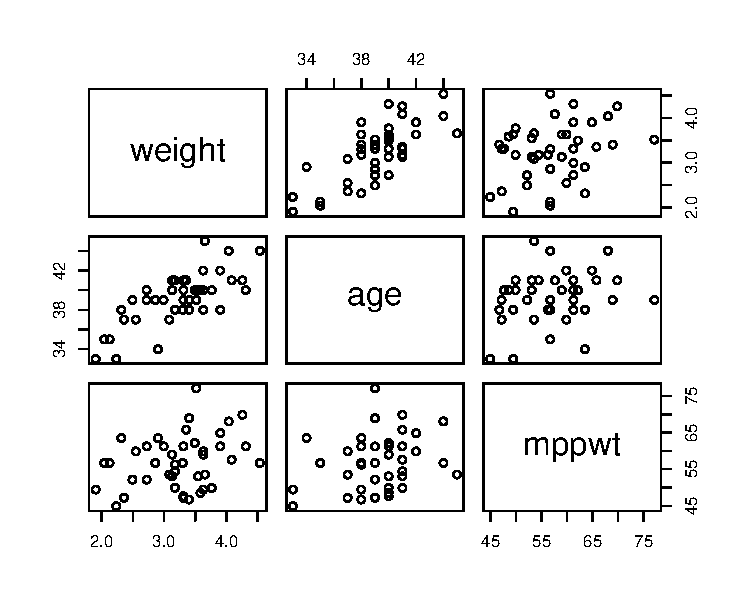
\includegraphics{MLG1_files/figure-latex/BWdataFig-1} 

}

\caption{Gráfico de dispersion del peso del recien nacido y la edad gestacional.}\label{fig:BWdataFig}
\end{figure}

\begin{Shaded}
\begin{Highlighting}[]
\FunctionTok{cor}\NormalTok{(birthweight[,}\FunctionTok{c}\NormalTok{(}\DecValTok{3}\NormalTok{,}\DecValTok{4}\NormalTok{,}\DecValTok{8}\NormalTok{)])}
\end{Highlighting}
\end{Shaded}

\begin{verbatim}
##           weight       age     mppwt
## weight 1.0000000 0.7311334 0.3048027
## age    0.7311334 1.0000000 0.2505155
## mppwt  0.3048027 0.2505155 1.0000000
\end{verbatim}

Por lo tanto, junto con la edad gestacional, ahora vamos a incluir peso de la madre antes del embarazo (en kgs, \texttt{mppwt}) como covariable. Por lo tanto, el modelo propuesto es:
\[
\mbox{weight}_{i} = \beta_{0} + \beta_{1}\mbox{age}_{i} + \beta_{2}\mbox{mppwt}_{i} + \varepsilon_{i}, \mbox{ para }i=1,\ldots,42,
\]
con \(\varepsilon_{i}\sim N(0,\sigma^{2})\), y \(cov(\varepsilon_{j},\varepsilon_{k})=0\) para todo \(j\neq k\).

\rule{\textwidth}{0.4pt}

\hypertarget{modelo-lineal-muxfaltiple-1}{%
\subsection{Modelo lineal múltiple}\label{modelo-lineal-muxfaltiple-1}}

En general, se puede relacionar la variable respuesta (\(y\)), con \(p-1\) covariables (o variables predictoras). El modelo lineal múltiple se expresa de la siguiente forma:

\begin{equation}
\begin{split}
y_{i} =& \beta_{0} + \beta_{1}x_{i1} + \beta_{2}x_{i2} + \ldots + \beta_{p-1} x_{i,p-1} + \varepsilon_{i} \\
=& \boldsymbol x_{i}'\boldsymbol \beta+ \varepsilon_{i}, \qquad i=1,\ldots,n, \\
\end{split}
\label{eq:modMultiple}
\end{equation}

donde \(\boldsymbol x_{i} = (1,x_{i1},x_{i2},\ldots,x_{i,p-1})'\) es el vector de dimensión \(p\) de covariables del individuo \(i\) y \(\boldsymbol \beta= (\beta_{0},\beta_{1},\ldots,\beta_{p-1})'\) es el vector de dimensión \(p\) de coeficientes de regresión.

Los supuestos del modelo son los mismos que se plantearon en el capítulo anterior. Estos es: \(\varepsilon_{i} \sim N\left(0,\sigma^{2} \right)\) y \(cov(\varepsilon_{j},\varepsilon_{k})=0\), para todo \(j \neq k\).

Dado que \(E(\varepsilon_{i})=0\), el valor esperado de \(Y\) es:
\begin{equation}
E(Y| x_{i1},x_{i2},\ldots,x_{i,p-1}) = E(Y| \boldsymbol x_{i}) = \beta_{0} + \beta_{1}x_{i1} + \beta_{2}x_{i2} + \ldots + \beta_{p-1} x_{i,p-1} = \boldsymbol x_{i}'\boldsymbol \beta.
\label{eq:expValue}
\end{equation}
El intercepto \(\beta_{0}\) es el valor esperado de \(Y\) cuando \(x_{i}=(1,0,0,\ldots,0)'\), es decir cuando todos las covariables toman el valor \(0\).

El parámetro de pendiente \(\beta_{j}\) indica el cambio en el valor esperado de \(Y\) debido a un aumento unitario en la covariable \(x_{j}\) cuando todas las demás variables predictoras se mantienen constantes. Sean \(x_{i,j} = (1,x_{i1},\ldots,x_{ij},\ldots,x_{i,p-1})\) y \(x_{i,j+1} = (1,x_{i1},\ldots,x_{ij}+1,\ldots,x_{i,p-1})\). A partir de \eqref{eq:expValue}, tenemos:
\[
E(Y|x_{i,j}) = \beta_{0} + \beta_{1}x_{i1} + \ldots + \beta_{j}x_{ij} + \ldots + \beta_{p-1} x_{i,p-1},
\]
y
\[
E(Y|x_{i,j+1}) = \beta_{0} + \beta_{1}x_{i1} + \ldots + \beta_{j}(x_{ij}+1) + \ldots + \beta_{p-1} x_{i,p-1}.
\]
De aquí tenemos que:
\[
E(Y|x_{i,j+1}) - E(Y|x_{i,j}) = \beta_{j}.
\]
Es conveniente escribir el modelo de regresión múltiple \eqref{eq:modMultiple} de forma matricial:
\[
\boldsymbol y= \boldsymbol X\boldsymbol \beta+ \boldsymbol \varepsilon,
\]
donde:
\begin{gather}
\begin{aligned}
\boldsymbol y= \begin{pmatrix}
y_{1} \\ y_{2} \\ \vdots \\ y_{n}
\end{pmatrix}, & \boldsymbol X= \begin{pmatrix}
1 & x_{11} & x_{12} & \ldots & x_{1,p-1} \\ 1 & x_{21} & x_{22} & \ldots & x_{2,p-1} \\ \vdots & \vdots & \vdots & \ddots & \vdots \\ 1 & x_{n1} & x_{n2} & \ldots & x_{n,p-1}
\end{pmatrix},
\boldsymbol \beta= \begin{pmatrix}
\beta_{0} \\ \beta_{1} \\ \beta_{2} \\ \vdots \\ \beta_{p-1}
\end{pmatrix}, & \boldsymbol \varepsilon= \begin{pmatrix}
\varepsilon_{1} \\ \varepsilon_{2} \\ \vdots \\ \varepsilon_{n}
\end{pmatrix}.
\end{aligned}
\nonumber
\end{gather}
Además, los supuestos sobre los errores se pueden expresar como \(\boldsymbol \varepsilon\sim N(\boldsymbol 0, \sigma^{2}\boldsymbol I)\), donde \(\boldsymbol 0\) es un vector con todas las entradas iguales a cero, y \(\boldsymbol I\) es la matriz identidad.

\hypertarget{estimaciuxf3n-de-los-paruxe1metros-de-regresiuxf3n}{%
\subsection{Estimación de los parámetros de regresión}\label{estimaciuxf3n-de-los-paruxe1metros-de-regresiuxf3n}}

La estimación de \(\boldsymbol \beta\) se hace a través del método de mínimos cuadrados ordinarios. Por lo tanto, debemos encontrar el vector \(\widehat{\boldsymbol \beta}\) que minimice:
\[
S(\boldsymbol \beta) =  \sum_{i=1}^{n}\left(y_{i} - \boldsymbol x_{i}'\boldsymbol \beta\right)^2 = \sum_{i=1}^{n}e_{i}^2.
\]
En forma matricial, tenemos:
\begin{equation}
\begin{split}
S(\boldsymbol \beta) &= \boldsymbol e'\boldsymbol e= (\boldsymbol y- \boldsymbol X\boldsymbol \beta)'(\boldsymbol y- \boldsymbol X\boldsymbol \beta) \\
&= \boldsymbol y'\boldsymbol y- \boldsymbol \beta'\boldsymbol X'\boldsymbol y- \boldsymbol y'\boldsymbol X\boldsymbol \beta+ \boldsymbol \beta'\boldsymbol X'\boldsymbol X\boldsymbol \beta\\
&= \boldsymbol y'\boldsymbol y- 2\boldsymbol \beta'\boldsymbol X'\boldsymbol y+ \boldsymbol \beta'\boldsymbol X'\boldsymbol X\boldsymbol \beta.
\end{split}
\nonumber
\end{equation}
Por lo tanto, \(\widehat{\boldsymbol \beta}\) debe satisfacer:
\[
\left. \frac{\partial S}{\partial \boldsymbol \beta} \right|_{\widehat{\boldsymbol \beta}} = - 2\boldsymbol X'\boldsymbol y+ 2\boldsymbol X'\boldsymbol X\widehat{\boldsymbol \beta}= \boldsymbol 0.
\]
A partir de aquí obtenemos las \textbf{ecuaciones normales}:
\[
\boldsymbol X'\boldsymbol X\widehat{\boldsymbol \beta}= \boldsymbol X'\boldsymbol y.
\]
En más detalle:
\begin{gather}
\begin{pmatrix}
n & \sum x_{i1} & \sum_{i=1}^{n}x_{i2} & \ldots & \sum_{i=1}^{n}x_{i,p-1} \\
\sum x_{i1} & \sum x_{i1}^2 & \sum x_{i1}x_{i2} & \ldots & \sum x_{i1}x_{i,p-1} \\
\sum x_{i2} & \sum x_{i1}x_{i2} & \sum x_{i2}^2 & \ldots & \sum x_{i2}x_{i,p-1} \\
\vdots & \vdots & \vdots & \ddots & \vdots \\
\sum x_{i,p-1} & \sum x_{i1}x_{i,p-1} & \sum x_{i2}x_{i,p-1} & \ldots & \sum x_{i,p-1}^{2} \\
\end{pmatrix} \begin{pmatrix}
\widehat{\beta}_{0} \\ \widehat{\beta}_{1} \\ \vdots \\ \widehat{\beta}_{p-1} \end{pmatrix} = \begin{pmatrix}
\sum y_{i} \\ \sum x_{i1}y_{i} \\ \vdots \\ \sum x_{i,p-1}y_{i}
\end{pmatrix}
\nonumber
\end{gather}
Por lo cual, el estimador por mínimos cuadrados es:
\[
\widehat{\boldsymbol \beta}= (\boldsymbol X'\boldsymbol X)^{-1}\boldsymbol X'\boldsymbol y.
\]
Note que es necesario que \(\boldsymbol X\) sea de rango completo, \(\mbox{rango}(\boldsymbol X) = p \leq n\). Esta restricción es necesaria para asegurar que \(\boldsymbol X'\boldsymbol X\) sea no singular. Si \(\boldsymbol X'\boldsymbol X\) es singular, implica que existe una combinación lineal entre las columnas de \(\boldsymbol X\), o que \(\mbox{rango}(\boldsymbol X) < p\).

El valor ajustado de \(y\) para el vector de covariables \(\boldsymbol x_{i}\) es \(\widehat{y}_{i}= \boldsymbol x_{i}'\widehat{\boldsymbol \beta}\). Definiendo \(\widehat{\boldsymbol y}= (\widehat{y}_{1},\widehat{y}_{2},\ldots,\widehat{y}_{n})\), tenemos que:
\[
\widehat{\boldsymbol y}= \boldsymbol X\widehat{\boldsymbol \beta}= \boldsymbol X(\boldsymbol X'\boldsymbol X)^{-1}\boldsymbol X'\boldsymbol y= \boldsymbol H\boldsymbol y.
\]
La matriz \((n\times n)\) \(\boldsymbol H= \boldsymbol X(\boldsymbol X'\boldsymbol X)^{-1}\boldsymbol X'\) es llamada \textbf{matriz hat} (sombrero) y desempeña un papel importante en el análisis de regresión.

Los residuos del modelo \((e_{i}=y_{i}-\widehat{y}_{i})\) también se pueden expresar en forma matricial:
\[
\boldsymbol e= \boldsymbol y- \boldsymbol X'\widehat{\beta}= \boldsymbol y- \boldsymbol X(\boldsymbol X'\boldsymbol X)^{-1}\boldsymbol X'\boldsymbol y= \boldsymbol y- \boldsymbol H\boldsymbol y= (\boldsymbol I_{n} - \boldsymbol H)\boldsymbol y.
\]

\hypertarget{estimaciuxf3n-de-sigma2-1}{%
\subsubsection{\texorpdfstring{Estimación de \(\sigma^{2}\)}{Estimación de \textbackslash sigma\^{}\{2\}}}\label{estimaciuxf3n-de-sigma2-1}}

Al igual que en la regresión simple, el estimador de \(\sigma^{2}\) es el cuadrado medio del error, definido como:
\[
MS_{res} = \frac{SS_{res}}{n-p},
\]
donde:
\begin{equation}
\begin{split}
SS_{res} &= \sum_{i=1}^{n}e^{2}_{i} = \boldsymbol e'\boldsymbol e= (\boldsymbol y- \boldsymbol X\widehat{\boldsymbol \beta})'(\boldsymbol y- \boldsymbol X\widehat{\boldsymbol \beta}) \\
&= (\boldsymbol y- \boldsymbol H\boldsymbol y)'(\boldsymbol y- \boldsymbol H\boldsymbol y) = \boldsymbol y'(\boldsymbol I_{n}-\boldsymbol H)'(\boldsymbol I_{n}-\boldsymbol H)\boldsymbol y= \boldsymbol y'(\boldsymbol I_{n} - \boldsymbol H)\boldsymbol y.
\end{split}
\nonumber
\end{equation}
Se puede demostrar que \(MS_{res}\) es un estimador insesgado de \(\sigma^{2}\), es decir \(E(MS_{res})=\sigma^{2}\). Para esto debemos calcular el valor esperado de \(SS_{res}\).

Sabemos que \(E(\boldsymbol y) = \boldsymbol X\boldsymbol \beta\) y \(V(\boldsymbol y) = \sigma^{2}\boldsymbol I_{n}\), entonces:
\[
E(SS_{res}) = E\left[\boldsymbol y'(\boldsymbol I_{n} - \boldsymbol H)\boldsymbol y\right] = \sigma^{2}\mbox{tr}\left( \boldsymbol I_{n} - \boldsymbol H\right) + \boldsymbol \beta'\boldsymbol X'(\boldsymbol I_{n} - \boldsymbol H)\boldsymbol X\boldsymbol \beta= (n-p)\sigma^{2}.
\]
Por lo tanto, \(E(MS_{res}) = E(SS_{res})/(n-p) = \sigma^{2}\).

\rule{\textwidth}{0.4pt}

\hypertarget{bajo-peso-al-nacer---estimaciuxf3n-de-paruxe1metros}{%
\subsubsection{Bajo peso al nacer - estimación de parámetros}\label{bajo-peso-al-nacer---estimaciuxf3n-de-paruxe1metros}}

Para ajustar el modelo:
\[
\mbox{weight}_{i} = \beta_{0} + \beta_{1}\mbox{age}_{i} + \beta_{2}\mbox{mppwt}_{i} + \varepsilon_{i}, \mbox{ para }i=1,\ldots,42,
\]
con \(\varepsilon_{i}\sim N(0,\sigma^{2})\), y \(cov(\varepsilon_{j},\varepsilon_{k})=0\) para todo \(j\neq k\), usamos la función \texttt{lm} de R:

\begin{Shaded}
\begin{Highlighting}[]
\NormalTok{mod }\OtherTok{=} \FunctionTok{lm}\NormalTok{(weight }\SpecialCharTok{\textasciitilde{}}\NormalTok{ age }\SpecialCharTok{+}\NormalTok{ mppwt, }\AttributeTok{data=}\NormalTok{birthweight)}
\NormalTok{mod}
\end{Highlighting}
\end{Shaded}

\begin{verbatim}
## 
## Call:
## lm(formula = weight ~ age + mppwt, data = birthweight)
## 
## Coefficients:
## (Intercept)          age        mppwt  
##    -3.97750      0.16746      0.01142
\end{verbatim}

De aquí temenos que:
\[
E(\mbox{weight} | \mbox{age}, \mbox{mppwt})= -3.978+0.167\mbox{age}+0.011\mbox{mppwt}.
\]
Aquí vemos que ambas covariables tienen un efecto positivo sobre el peso del bebé al nacer. Especificamente, tenemos que:

\begin{itemize}
\tightlist
\item
  Si la edad gestacional aumenta en una semana y el peso de la madre se mantiene constante, el valor esperado del peso al nacer crece 167 gramos.
\item
  Por cada incremento de un kilogramo en el peso de la madre y manteniendo la edad gestacional constante, el peso al nacer medio aumenta 11 gramos.
\end{itemize}

Además, la estimación de \(\sigma^{2}\) es:

\begin{Shaded}
\begin{Highlighting}[]
 \FunctionTok{sqrt}\NormalTok{(}\FunctionTok{sum}\NormalTok{(mod}\SpecialCharTok{$}\NormalTok{residuals}\SpecialCharTok{\^{}}\DecValTok{2}\NormalTok{)}\SpecialCharTok{/}\DecValTok{39}\NormalTok{)}
\end{Highlighting}
\end{Shaded}

\begin{verbatim}
## [1] 0.4356247
\end{verbatim}

Note que al adicionar la covariable \texttt{mppwt} se redujo el \(MS_{res}\).

\rule{\textwidth}{0.4pt}

\hypertarget{propiedades-de-los-estimadores-por-mco-1}{%
\subsubsection{Propiedades de los estimadores por MCO}\label{propiedades-de-los-estimadores-por-mco-1}}

El valor esperado de \(\widehat{\boldsymbol \beta}\) es:
\begin{equation}
\begin{split}
E(\widehat{\boldsymbol \beta}) =& E\left[ (\boldsymbol X'\boldsymbol X)^{-1}\boldsymbol X'\boldsymbol y\right] = E\left[ \boldsymbol X'\boldsymbol X)^{-1}\boldsymbol X'(\boldsymbol X\boldsymbol \beta+ \boldsymbol \varepsilon) \right] \\
=& E\left[ (\boldsymbol X'\boldsymbol X)^{-1}\boldsymbol X'\boldsymbol X\boldsymbol \beta+ (\boldsymbol X'\boldsymbol X)^{-1}\boldsymbol X'\boldsymbol \varepsilon\right] = \boldsymbol \beta
\end{split}
\nonumber
\end{equation}
Por lo tanto, \(\widehat{\boldsymbol \beta}\) es un estimador insesgado de \(\boldsymbol \beta\) (si el modelo está bien espeficado).

La matriz de varianzas-covarianzas de \(\widehat{\boldsymbol \beta}\) es:
\begin{equation}
\begin{split}
V(\widehat{\boldsymbol \beta}) &= V\left[ (\boldsymbol X'\boldsymbol X)^{-1}\boldsymbol X'\boldsymbol y\right] = (\boldsymbol X'\boldsymbol X)^{-1}\boldsymbol X'V(\boldsymbol y)\boldsymbol X(\boldsymbol X'\boldsymbol X)^{-1}  \\
&= \sigma^{2}(\boldsymbol X'\boldsymbol X)^{-1}\boldsymbol X'\boldsymbol X(\boldsymbol X'\boldsymbol X)^{-1} = \sigma^{2}(\boldsymbol X'\boldsymbol X)^{-1}.
\end{split}
\nonumber
\end{equation}
Si \(\boldsymbol C=(\boldsymbol X'\boldsymbol X)^{-1}\), entonces \(V(\widehat{\beta}_{j}) = \sigma^{2}c_{jj}\) y \(Cov(\widehat{\beta}_{j},\widehat{\beta}_{k})=\sigma^{2}c_{jk}\), donde \(c_{jk}\) es la entrada \((j,k)\) de la matriz \(\boldsymbol C\).

\hypertarget{teorema-de-gauss-markov}{%
\paragraph*{Teorema de Gauss-Markov}\label{teorema-de-gauss-markov}}
\addcontentsline{toc}{paragraph}{Teorema de Gauss-Markov}

Si, \(E(\boldsymbol \varepsilon) = \boldsymbol 0\) y \(V(\boldsymbol \varepsilon) = \sigma^{2}\boldsymbol I_{n}\), el estimador por MCO, \(\widehat{\boldsymbol \beta}= (\boldsymbol X'\boldsymbol X)\boldsymbol X'\boldsymbol y\), es el mejor estimador lineal insesgado de \(\boldsymbol \beta\). Esto quiere decir que es el estimador con menor varianza entre la clase de estimador insesgados que son combinaciones lineales de \(y\). Para la demostración, ver Sección C4 de \citet{montgomery_introduction_2012}.

Además, si \(\boldsymbol \varepsilon\sim N(\boldsymbol 0, \sigma^{2}\boldsymbol I_{n})\), el estimador por MCO coincide con el estimador por máxima verosimilitud.

\hypertarget{pruebas-de-hipuxf3tesis-1}{%
\subsection{Pruebas de hipótesis}\label{pruebas-de-hipuxf3tesis-1}}

Después de estimar el modelo podemos preguntarnos:

\begin{itemize}
\tightlist
\item
  ¿el modelo hace un buen ajuste de los datos?
\item
  ¿cuales regresores específicos parecen importantes?
\end{itemize}

Para resolver estas preguntas podemos realizar pruebas de hipótesis. Generalmente, estos test requieren que \(\boldsymbol \varepsilon\sim N(\boldsymbol 0,\sigma^{2}\boldsymbol I_{n})\).

\hypertarget{anuxe1lisis-de-varianza-1}{%
\subsubsection{Análisis de varianza}\label{anuxe1lisis-de-varianza-1}}

Para probar la significancia del modelo (determinar si que la relación entre \(y\) y algunas de las covariables es lineal) se plantean las siguientes hipótesis:
\begin{equation}
\begin{split}
H_{0}:& \beta_{1}=\beta_{2}=\ldots=\beta_{p-1} = 0 \\
H_{1}:& \beta_{j}\neq 0 \mbox{ para al menos un }j.
\end{split}
\label{eq:HANOVA}
\end{equation}
El rechazo de esta hipótesis nula implica que al menos uno de los regresores \(x_1, x_2,\ldots , x_{p-1}\) contribuye significativamente al modelo.

Igual que en la regresión simple, el estadístico de prueba se encuentra a partir de la partición de la suma de cuadrados totales:
\[
SS_{T}  = SS_{R} + SS_{res},
\]
donde:

\begin{itemize}
\tightlist
\item
  \(SS_{T} = \sum_{i=1}^{n}(y_{i}-\bar{y})^{2} = (\boldsymbol y- \frac{1}{n}\boldsymbol 1'\boldsymbol y)'(\boldsymbol y- \frac{1}{n}\boldsymbol 1'\boldsymbol y)\),
\item
  \(SS_{R} = \sum_{i=1}^{n}(\widehat{y}_{i}-\bar{y})^{2} = (\boldsymbol H\boldsymbol y- \frac{1}{n}\boldsymbol 1'\boldsymbol y)'(\boldsymbol H\boldsymbol y- \frac{1}{n}\boldsymbol 1'\boldsymbol y)\),
\item
  \(SS_{res} = \sum_{i=1}^{n}(y_{i}-\widehat{y}_{i})^{2} = (\boldsymbol y- \boldsymbol H\boldsymbol y)'(\boldsymbol y- \boldsymbol H\boldsymbol y)\),
\end{itemize}

y \(\boldsymbol 1\) es un vector cuyas entradas son iguales a \(1\).

Si \(H_{0}\) es cierta, tenemos que:
\[
\frac{SS_{res}}{\sigma^{2}}\sim\chi^{2}_{n-p} \mbox{ y } \frac{SS_{R}}{\sigma^{2}} \sim \chi^{2}_{p-1},
\]
además, \(SS_{res}\) y \(SS_{R}\) son independientes. Por lo tanto,
\[
F_{0} = \frac{SS_{R}/(p-1)}{SS_{res}/(n-p)} = \frac{MS_{R}}{MS_{res}} \sim F_{p-1,n-p}.
\]
También se puede probar que:
\[
E(MS_{res}) =  \sigma^{2} \mbox{ y }E(MS_{R}) =  \sigma^{2} + \frac{\boldsymbol \beta^{*'}\boldsymbol X_{c}'\boldsymbol X_{c}\boldsymbol \beta^{*}}{(p-1)\sigma^{2}},
\]
donde \(\boldsymbol \beta^{*} = (\beta_{1},\beta_{2},\ldots,\beta_{p-1})'\) y
\[
\boldsymbol X_{c} = \begin{pmatrix}
x_{11} - \bar{x}_{1} & x_{12} - \bar{x}_{2} & \ldots & x_{1,p-1} - \bar{x}_{p-1} \\ 
x_{21} - \bar{x}_{1} & x_{22} - \bar{x}_{2} & \ldots & x_{2,p-1} - \bar{x}_{p-1} \\ 
\vdots & \vdots & \ddots & \vdots \\
x_{i1} - \bar{x}_{1} & x_{i2} - \bar{x}_{2} & \ldots & x_{i,p-1} - \bar{x}_{p-1} \\ 
\vdots & \vdots & \ddots & \vdots \\
x_{n1} - \bar{x}_{1} & x_{n2} - \bar{x}_{2} & \ldots & x_{n,p-1} - \bar{x}_{p-1} \\ 
\end{pmatrix}.
\]

Si \(H_{0}\) no es cierta, tenemos que \(F_{0}\) sigue una distribución \(F\) no-central con \(p-1\) y \(n-p\) grados de libertad y parámetro de no centralidad:
\[
\lambda = \frac{\boldsymbol \beta'\boldsymbol X_{c}'\boldsymbol X_{c}\boldsymbol \beta}{\sigma^{2}}.
\]
Estos nos resultados nos indican que si el valor \(F_{0}\) es grande, entonces al menos un \(\beta_{j}\) es diferente de cero.

Por lo tanto, para probar las hipótesis \eqref{eq:HANOVA} calculamos el estadístico de prueba \(F_{0} = \frac{MS_{R}}{MS_{res}}\), y rechazamos \(H_{0}\) si \(F_{0} > F_{1-\alpha,p-1,n-p}\).

A partir de las sumas de cuadrados podemos calcular el coeficiente de determinación:
\[
R^{2} = 1-\frac{SS_{res}}{SS_{T}}.
\]
A medida que agregamos mas covariables al modelo el \(R^{2}\) aumenta (o permanece igual), sin importar si la covariable agregada tiene una contribución importante en el ajuste. Esto hace que sea difícil determinar si el incremento en el \(R^{2}\) al agregar una covariable sea relevante. Por esta razón, también podemos usar el coeficiente de determinación ajustado:
\[
R^{2}_{adj} = 1-\frac{SS_{res}/(n-p)}{SS_{T}/(n-1)} = 1 - \frac{MS_{res}}{SS_T/(n-1)}.
\]
Aunque no tiene interpretación, el \(R^{2}_{adj}\) puede usarse para comparar modelos al agregar covariables. Dado que \(SS_{T}/(n-1)\) es constante, el \(R^{2}_{adj}\) solo aumentará al agregar una covariable nueva al modelo si la adición de la covariable reduce el \(MS_{res}\).

\hypertarget{pruebas-individuales-sobre-los-coeficientes}{%
\subsubsection{Pruebas individuales sobre los coeficientes}\label{pruebas-individuales-sobre-los-coeficientes}}

Al rechazar \(H_{0}\) de la prueba de hipótesis \eqref{eq:HANOVA} concluimos que al menos un coeficiente es diferente de cero. Por lo tanto, una o más covariables tienen un aporte significativo en el modelo. El paso que sigue es identificar estas covariables.

Para esto podemos plantear las siguientes hipótesis individuales sobre los coeficientes del modelo:
\[
H_{0}: \beta_{j} = 0 \qquad H_{1}: \beta_{j} \neq 0.
\]
El estadística de prueba es:
\[
t_{0} = \frac{\widehat{\beta}_{j}}{se(\widehat{\beta}_{j})} = \frac{\widehat{\beta}_{j}}{\sqrt{MS_{res}c_{jj}}},
\]
donde \(c_{jj}\) es la entrada \((j,j)\) de la matriz \(\boldsymbol C= (\boldsymbol X'\boldsymbol X)^{-1}\). Rechazamos \(H_{0}\) si \(|t_{0}| > t_{1-\alpha/2,n-p}\).

Este es una prueba parcial, puesto que estamos evaluando la significancia de \(x_{j}\) cuando las demás covariables \(x_{k}\), para \(k\neq j\), ya están incluidas en el modelo. Por lo tanto, si no rechazamos \(H_{0}\), podemos concluir que, cuando los demás regresores están en el modelo, la covariable \(x_{j}\) no tiene un aporte significativo. Por lo tanto, podríamos retirarla del modelo.

\hypertarget{pruebas-sobre-subconjuntos-de-coeficientes}{%
\subsubsection{Pruebas sobre subconjuntos de coeficientes}\label{pruebas-sobre-subconjuntos-de-coeficientes}}

Para probar la significancia de un subconjunto de coeficientes del modelo hacemos uso de la \textbf{suma de cuadrados extra}. Primero, consideremos el siguiente modelo de regresión:
\[
\boldsymbol y= \boldsymbol X\boldsymbol \beta+ \boldsymbol \varepsilon,
\]
donde \(\boldsymbol X\) es una matrix \(n \times p\) y \(\boldsymbol \beta\) es el vector de coeficientes de longitud \(p\). Queremos probar si un subconjunto \(r < p\) de covariables tienen un aporte significativo en el modelo. Para esto hacemos la siguiente partición del vector \(\boldsymbol \beta\):
\[
\boldsymbol \beta= \begin{pmatrix} \beta_{0} \\ \beta_{1} \\ \vdots \\ \beta_{p-r-1} \\ \hline \beta_{p-r} \\ \beta_{p-r+1} \\ \vdots \\  \beta_{p} \end{pmatrix} =  \begin{pmatrix} \boldsymbol \beta_{1} \\ \hline \boldsymbol \beta_{2}\end{pmatrix},
\]
donde \(\boldsymbol \beta_{1}\) y \(\boldsymbol \beta_{2}\) son vector de dimensión \((p-r)\) y \((r)\), respectivamente. Por lo tanto, queremos realizar la siguiente prueba de hipótesis:
\begin{equation}
H_{0}:  \boldsymbol \beta_{2} = \boldsymbol 0\qquad H_{1}:  \boldsymbol \beta_{2} \neq \boldsymbol 0.
\label{eq:Hsubset}
\end{equation}
El modelo anterior se puede re-escribir de la siguiente forma:
\[
\boldsymbol y= \boldsymbol X\boldsymbol \beta+ \boldsymbol \varepsilon= \boldsymbol X_{1}\boldsymbol \beta_{1}+ \boldsymbol X_{2}\boldsymbol \beta_{2} + \boldsymbol \varepsilon,
\]
donde \(\boldsymbol X_{1}\) es la matriz \(n\times (p-r)\) que contiene las columnas de \(\boldsymbol X\) asociadas con \(\boldsymbol \beta_{1}\), y \(\boldsymbol X_{2}\) es la matriz \(n\times r\) que contiene las columnas de \(\boldsymbol X\) asociadas con \(\boldsymbol \beta_{2}\). Este es llamado el \textbf{modelo completo}.

Para el modelo completo tenemos:

\begin{itemize}
\tightlist
\item
  Estimador de \(\boldsymbol \beta\):
  \[
  \widehat{\boldsymbol \beta}= (\boldsymbol X'\boldsymbol X)^{-1}\boldsymbol X'\boldsymbol y.
  \]
\item
  Suma de cuadrados del modelo:
  \[
  SS_{R}(\boldsymbol \beta) = \widehat{\beta}'\boldsymbol X'\boldsymbol y\mbox{ (con }p\mbox{ grados de libertad)}.
  \]
\item
  Cuadrado medio del error:
  \[
  MS_{res} = \frac{\boldsymbol y'\boldsymbol y- \widehat{\boldsymbol \beta}'\boldsymbol X'\boldsymbol y}{n-p}.
  \]
\end{itemize}

Para evaluar la contribución de los regresores asociados a \(\boldsymbol \beta_{2}\), ajustamos el modelo asumiendo que \(H_{0}\) es cierta. De esta forma tenemos el \textbf{modelo reducido}:
\[
\boldsymbol y= \boldsymbol X_{1}\boldsymbol \beta_{1} + \boldsymbol \varepsilon.
\]
Para el modelo reducido tenemos:

\begin{itemize}
\tightlist
\item
  Estimador de \(\boldsymbol \beta_{1}\):
  \[
  \widehat{\boldsymbol \beta}_{1} = (\boldsymbol X_{1}'\boldsymbol X_{1})^{-1}\boldsymbol X_{1}'\boldsymbol y.
  \]
\item
  Suma de cuadrados del modelo:
  \[
  SS_{R}(\boldsymbol \beta_{1}) = \widehat{\boldsymbol \beta}_{1}'\boldsymbol X_{1}'\boldsymbol y\mbox{ (con $p-r$ grados de libertad)}.
  \]
\end{itemize}

Entonces, la suma de cuadrados debido a \(\boldsymbol \beta_{2}\) dado que \(\boldsymbol \beta_{1}\) ya está en el modelo es:
\[
SS_{R}(\boldsymbol \beta_{2}| \boldsymbol \beta_{1}) = SS_{R}(\boldsymbol \beta) - SS_{R}(\boldsymbol \beta_{1}),
\]
con \(p-(p-r)=r\) grados de libertad. Esta suma de cuadrados es llamada la suma de cuadrados extra debido a \(\boldsymbol \beta_2\) puesto que mide el incremento en la suma de cuadrados de la regresión como resultado de adicionar los regresores \(\boldsymbol X_{2}\) en el modelo que ya contiene \(\boldsymbol X_{1}\).

Dado que \(SS_{R}(\boldsymbol \beta_{2}| \boldsymbol \beta_{1})\) y \(MS_{res}\) son independientes, podemos utilizar el siguiente estadístico de prueba:
\[
F_{0} = \frac{SS_{R}(\boldsymbol \beta_{2}|\boldsymbol \beta_{1})/r}{MS_{res}}.
\]
Si \(H_{0}\) es cierta entonces \(F_{0} \sim F_{r,n-p}\). Si \(H_{0}\) no es cierta, entonces \(F_{0}\) sigue una distribución \(F\) no-central con parámetro de no centralidad igual a:
\[
\lambda = \frac{1}{\sigma^{2}}\boldsymbol \beta_{2}'\boldsymbol X_{2}'\left[ \boldsymbol I_{n} - \boldsymbol X_{1}(\boldsymbol X_{1}'\boldsymbol X_{1})^{-1}\boldsymbol X_{1}'\right]\boldsymbol X_{2}\boldsymbol \beta_{2}.
\]
Note que si hay una relación casi colineal entre \(\boldsymbol X_{1}\) y \(\boldsymbol X_{2}\) (multicolinealidad), \(\lambda\) es cercano a cero pesar que \(\boldsymbol \beta_{2}\) sea marcadamente distinto de cero. Es decir, que la prueba tiene poca capacidad de indicar diferencias (poco poder) en presencia de multicolinealidad. Caso contrario, el máximo poder se alcanza cuando \(\boldsymbol X_{1}\) y \(\boldsymbol X_{2}\) son ortogonales (es decir \(\boldsymbol X_{2}'\boldsymbol X_{1} = \boldsymbol 0\)).

Entonces, si \(F_{0} > F_{1-\alpha,r,n-p}\) rechazamos \(H_{0}\) y concluimos que al menos un coeficiente en \(\boldsymbol \beta_{2}\) es diferente de cero. Consecuentemente, al menos una de las covariables en \(\boldsymbol X_{2}\) tiene un aporte significativo dentro del modelo.

\hypertarget{ejemplo}{%
\paragraph*{Ejemplo}\label{ejemplo}}
\addcontentsline{toc}{paragraph}{Ejemplo}

Considere el modelo:
\[
y_{i} = \beta_{0} + \beta_{1}x_{i1} + \beta_{2}x_{i2} + \beta_{3}x_{i3} + \varepsilon_{i}.
\]
La suma de cuadrados del modelo se puede descomponer de la siguiente forma:
\[
SS_{R}=SS_{R}(\beta_{1},\beta_{2},\beta_{3}| \beta_{0}) = SS_{R}(\beta_{1}|\beta_{0}) + SS_{R}(\beta_{2}|\beta_{0},\beta_{1}) + SS_{R}(\beta_{3}|\beta_{0},\beta_{1},\beta_{2}),
\]
donde cada suma de cuadrados en el lado derecho tiene un grado de libertad. Además, el order de los regresores en estos componentes marginales es arbitrario. Por lo que la siguiente descomposición alternativa es también válida:
\[
SS_{R}(\beta_{1},\beta_{2},\beta_{3}| \beta_{0})=SS_{R}(\beta_{2}|\beta_{0}) + SS_{R}(\beta_{3}|\beta_{0},\beta_{2}) + SS_{R}(\beta_{1}|\beta_{0},\beta_{2},\beta_{3}).
\]

Sin embargo, la siguiente partición de la suma de cuadrados de la regrsión es generalmente inválida:
\[
SS_{R}(\beta_{1},\beta_{2},\beta_{3}| \beta_{0})\neq SS_{R}(\beta_{1}|\beta_{0},\beta_{2},\beta_{3}) + SS_{R}(\beta_{2}|\beta_{0},\beta_{1},\beta_{3}) + SS_{R}(\beta_{3}|\beta_{0},\beta_{1},\beta_{2}).
\]

\hypertarget{prueba-de-hipuxf3tesis-lineal-general}{%
\subsection{Prueba de hipótesis lineal general}\label{prueba-de-hipuxf3tesis-lineal-general}}

Suponga que estamos interesados en las siguientes hipótesis:
\begin{equation}
H_{0}: \boldsymbol T\boldsymbol \beta=\boldsymbol 0\qquad H_{1}: \boldsymbol T\boldsymbol \beta\neq \boldsymbol 0,
\label{eq:hipGeneral1}
\end{equation}
donde \(\boldsymbol T\) es una matriz \(m \times p\) de constantes, tal que \(r\) de las \(m\) ecuaciones de \(\boldsymbol T\boldsymbol \beta=\boldsymbol 0\) son independientes.

El \textbf{modelo completo (FM)} es:
\[
\boldsymbol y=\boldsymbol X\boldsymbol \beta+\boldsymbol \varepsilon,
\]
El estimador de \(\boldsymbol \beta\) es \(\widehat{\boldsymbol \beta}= (\boldsymbol X'\boldsymbol X)^{-1}\boldsymbol X'\boldsymbol y\), y la suma de cuadrados de los residuos es \(SS_{res}(FM)\) (con \(n-p\) grados de libertad).

El \textbf{modelo reducido (RM)} se obtiene al resolver las \(r\) ecuaciones independientes de \(\boldsymbol T\boldsymbol \beta= \boldsymbol 0\) para los \(r\) coeficientes en el modelo completo en términos de los \(p-r\) coeficientes restantes. Esto lleva al siguiente RM:
\[
\boldsymbol y=\boldsymbol Z\boldsymbol \gamma+\boldsymbol \varepsilon,
\]
donde \(\boldsymbol Z\) es una matriz \(n\times (p-r)\) y \(\boldsymbol \gamma\) es un vector de dimiensión \((p-r)\) de coeficientes de regresión. La suma de cuadrados de los residuos de este modelo es \(SS_{res}(RM)\) (con \(n-p+r\) grados de libertad).

Dado que el modelo reducido tiene menos parámetros que el modelo completo, \(SS_{res}(RM) \geq SS_{res}(FM)\). Para probar \eqref{eq:hipGeneral1} usamos la diferencia entre las sumas de cuadrados de los residuos:
\[
SS_{H} = SS_{res}(RM) - SS_{res}(FM),
\]
con \(r\) grados de libertad. \(SS_{H}\) es llamado la suma de cuadrados debido a \(H_{0}:\boldsymbol T\boldsymbol \beta=\boldsymbol c\). El estadístico de prueba es:
\[
F_{0} = \frac{SS_{H}/r}{SS_{res}(FM)/(n-p)} = \frac{\widehat{\beta}'\boldsymbol T[\boldsymbol T(\boldsymbol X'\boldsymbol X)\boldsymbol T']^{-1}\boldsymbol T\widehat{\boldsymbol \beta}/r}{SS_{res}(FM)/(n-p)}.
\]
Rechazamos \(H_{0}\) si \(F_{0} > F_{1-\alpha,r,n-p}\).

La hipótesis anterior se puede generalizar de la siguiente forma:
\begin{equation}
H_{0}: \boldsymbol T\boldsymbol \beta=\boldsymbol c\qquad H_{1}: \boldsymbol T\boldsymbol \beta\neq \boldsymbol c,
\label{eq:hipGeneral2}
\end{equation}
Para este caso, el estadístico de prueba es:
\[
F_{0} = \frac{(\boldsymbol T\widehat{\boldsymbol \beta}-\boldsymbol c)'[\boldsymbol T(\boldsymbol X'\boldsymbol X)\boldsymbol T']^{-1}(\boldsymbol T\widehat{\boldsymbol \beta}-\boldsymbol c)/r}{SS_{res}(FM)/(n-p)}.
\]
Si \(H_{0}\) es cierta, \(F_{0}\sim F_{r,n-p}\). Por lo tanto, rechazamos \(H_{0}\) si \(F_{0} > F_{1-\alpha,r,n-p}\).

\hypertarget{ejemplo-1}{%
\paragraph*{ejemplo}\label{ejemplo-1}}
\addcontentsline{toc}{paragraph}{ejemplo}

Considere el modelo:
\[
y_{i} = \beta_{0} + \beta_{1}x_{i1}+ \beta_{2}x_{i2}+ \beta_{3}x_{i3}+ \beta_{3}x_{i3} + \varepsilon_{i},
\]
y queremos probar las siguientes hipótesis:
\begin{align*}
H_{0}:& \beta_{1}=0 & H_{1}:&\beta_{1}\neq 0 \\
      & 2\beta_{2}-\beta_{3}=3 & &2\beta_{2}-\beta_{3}\neq 3 \\
\end{align*}
De aquí tenemos que:
\[
\boldsymbol T= \begin{pmatrix}
1 & 0 & 0 & 0 \\
0 & 2 & -1 & 0 \\
\end{pmatrix} \mbox{ y } \boldsymbol c= \begin{pmatrix} 0 \\ 3  \end{pmatrix}.
\]
Si no rechazamos \(H_{0}\), podríamos estimar \(\boldsymbol \beta\) sujo a las restricciones impuestar por la hipótesis nula (usando mínimos cuadrados restringidos).

\rule{\textwidth}{0.4pt}

\hypertarget{bajo-peso-al-nacer---pruebas-de-hipuxf3tesis}{%
\subsubsection*{Bajo peso al nacer - pruebas de hipótesis}\label{bajo-peso-al-nacer---pruebas-de-hipuxf3tesis}}
\addcontentsline{toc}{subsubsection}{Bajo peso al nacer - pruebas de hipótesis}

Los resultados de las pruebas de hipótesis individuales sobre los coeficientes, análisis de varianza y coeficientes de determianción se obtiene a partir del resumen del modelo:

\begin{Shaded}
\begin{Highlighting}[]
\FunctionTok{summary}\NormalTok{(mod)}
\end{Highlighting}
\end{Shaded}

\begin{verbatim}
## 
## Call:
## lm(formula = weight ~ age + mppwt, data = birthweight)
## 
## Residuals:
##      Min       1Q   Median       3Q      Max 
## -0.79566 -0.34083  0.05415  0.26504  0.88930 
## 
## Coefficients:
##              Estimate Std. Error t value Pr(>|t|)    
## (Intercept) -3.977501   1.053336  -3.776 0.000531 ***
## age          0.167456   0.026585   6.299 1.99e-07 ***
## mppwt        0.011416   0.009756   1.170 0.249032    
## ---
## Signif. codes:  0 '***' 0.001 '**' 0.01 '*' 0.05 '.' 0.1 ' ' 1
## 
## Residual standard error: 0.4356 on 39 degrees of freedom
## Multiple R-squared:  0.5503, Adjusted R-squared:  0.5273 
## F-statistic: 23.87 on 2 and 39 DF,  p-value: 1.703e-07
\end{verbatim}

A partir de estos resutados tenemos que \(F_{0}=23.8665\) con un valor-\(p\) asociado de \(0.000\), es decir que al menos uno de los coeficientes de regresión es diferente de cero. Además, el \(55\)\% de la variabilidad del peso al nacer es explicada por la edad gestacional y el peso de la madre antes del embarazo \((R^{2}=0.5503)\). Note que hubo un incremento leve en el \(R^{2}\) respecto al modelo que solo incluye la edad gestacional como covariable (\(R^{2} = 0.535\)).

A partir de las pruebas de hipótesis individuales, podemos decir que el peso de la madre antes del embarazo no tiene un aporte significativo cuando el modelo ya incluye la covariable edad gestacional (\(t_{0}=1.17\) con un valor-\(p\) asociado de 0.249). Por otro lado, el efecto de la edad gestacional si es significativo (\(t_{0}=6.3\) con un valor-\(p\) asociado de 0).

Ahora consideremos un modelo ingresando dos covariables más:
\[
y_{i} = \beta_{0} + \beta_{1}\mbox{age}_{i} + \beta_{2}\mbox{mppwt}_{i} + \beta_{3}\mbox{motherage}_{i} + \beta_{2}\mbox{mnocig}_{i} + \varepsilon_{i},
\]
donde \(\mbox{motherage}_{i}\) y \(\mbox{mnocig}_{i}\) es la edad (en años) y el número medio de cigarrillos fumados por mes de la \(i\)-ésima madre, respectivamente. El resumen del modelo ajustado es:

\begin{Shaded}
\begin{Highlighting}[]
\NormalTok{mod.completo }\OtherTok{=} \FunctionTok{lm}\NormalTok{(weight}\SpecialCharTok{\textasciitilde{}}\NormalTok{age }\SpecialCharTok{+}\NormalTok{ mppwt }\SpecialCharTok{+}\NormalTok{ motherage }\SpecialCharTok{+}\NormalTok{ mnocig,}\AttributeTok{data=}\NormalTok{birthweight)}
\FunctionTok{summary}\NormalTok{(mod.completo)}
\end{Highlighting}
\end{Shaded}

\begin{verbatim}
## 
## Call:
## lm(formula = weight ~ age + mppwt + motherage + mnocig, data = birthweight)
## 
## Residuals:
##      Min       1Q   Median       3Q      Max 
## -0.78765 -0.35948  0.09209  0.35024  0.75018 
## 
## Coefficients:
##              Estimate Std. Error t value Pr(>|t|)    
## (Intercept) -4.104029   1.011723  -4.056 0.000247 ***
## age          0.168027   0.024916   6.744 6.24e-08 ***
## mppwt        0.014838   0.009530   1.557 0.127966    
## motherage    0.001751   0.012335   0.142 0.887900    
## mnocig      -0.014417   0.005421  -2.660 0.011493 *  
## ---
## Signif. codes:  0 '***' 0.001 '**' 0.01 '*' 0.05 '.' 0.1 ' ' 1
## 
## Residual standard error: 0.4073 on 37 degrees of freedom
## Multiple R-squared:  0.627,  Adjusted R-squared:  0.5867 
## F-statistic: 15.55 on 4 and 37 DF,  p-value: 1.5e-07
\end{verbatim}

Respecto al modelo anterior, hay un aumento del \(R^{2}\) y el \(R^{2}_{adj}\). Por lo cuál podemos concluir que al ingresar estas covariables el ajuste mejoró. Aunque, los efectos del peso y la edad de la madre no son significativos a partir de las pruebas individuales.

Esto no necesariamente quiere decir que podemos eliminar estas dos covariables del modelo, recordemos que las pruebas \(t\) son individuales (se evalúa el efecto de la covariable cuando el modelo ya incluye las restantes). Para determinar si podemos eliminar \texttt{mppwt} y \texttt{motherage} del modelo, realizamos la siguiente prueba de hipótesis:
\[
H_{0}: \beta_{2} = \beta_{3} = 0 \qquad H_{0}: \beta_{j} \neq 0 \mbox{ para algún }j=2,3.
\]
En R podemos hacer esto a través de la función \texttt{anova}:

\begin{Shaded}
\begin{Highlighting}[]
\NormalTok{mod.reducido }\OtherTok{=} \FunctionTok{lm}\NormalTok{(weight}\SpecialCharTok{\textasciitilde{}}\NormalTok{age }\SpecialCharTok{+}\NormalTok{ mnocig,}\AttributeTok{data=}\NormalTok{birthweight)}
\FunctionTok{anova}\NormalTok{(mod.reducido,mod.completo)}
\end{Highlighting}
\end{Shaded}

\begin{verbatim}
## Analysis of Variance Table
## 
## Model 1: weight ~ age + mnocig
## Model 2: weight ~ age + mppwt + motherage + mnocig
##   Res.Df    RSS Df Sum of Sq      F Pr(>F)
## 1     39 6.5912                           
## 2     37 6.1386  2   0.45258 1.3639 0.2682
\end{verbatim}

Aquí vemos que \(F_{0}= 1.364\) con un valor-\(p\) asociado de \(0.2682\). Por lo tanto, no tenemos evidencia suficiente para rechazar \(H_{0}\) y podemos retirar las dos covariables del modelo.

\rule{\textwidth}{0.4pt}

\hypertarget{intervalos-de-confianza-1}{%
\subsection{Intervalos de confianza}\label{intervalos-de-confianza-1}}

Al igual que en caso del modelo lineal simple, también podemos hacer estimaciones por intervalos de confianza para los coeficientes del modelo, valor esperado de \(Y\) y observaciones futuras.

Para que los intervalos de confianza sean válidos se requiere que se cumplan todos los supuestos del modelo, esto es \(\boldsymbol \varepsilon\sim N(\boldsymbol 0, \sigma^{2}\boldsymbol I_{n})\).

\hypertarget{intervalos-de-confianza-para-beta_j}{%
\subsubsection{\texorpdfstring{Intervalos de confianza para \(\beta_{j}\)}{Intervalos de confianza para \textbackslash beta\_\{j\}}}\label{intervalos-de-confianza-para-beta_j}}

El intervalo de confianza de \(\beta_{j}\) parte de:
\[
\frac{\widehat{\beta}_{j} - \beta_{j}}{\sqrt{V(\widehat{\beta}_{j})}} =  \frac{\widehat{\beta}_{j} - \beta_{j}}{\sqrt{MS_{res}c_{jj}}} \sim t_{n-p},
\]
donde \(c_{jj}\) es la entrada \((j,j)\) de la matriz \(\boldsymbol C=(\boldsymbol X'\boldsymbol X)^{-1}\). Entonces, el intervalo del \((1-\alpha)100\%\) de confianza para \(\widehat{\beta}_{j}\) es:
\[
\widehat{\beta}_{j} \pm t_{1-\alpha/2,n-p}\sqrt{MS_{res}c_{jj}}.
\]

\hypertarget{intervalos-de-confianza-para-el-valor-esperado-de-y-y-una-observaciuxf3n-futura}{%
\subsubsection{\texorpdfstring{Intervalos de confianza para el valor esperado de \(Y\) y una observación futura}{Intervalos de confianza para el valor esperado de Y y una observación futura}}\label{intervalos-de-confianza-para-el-valor-esperado-de-y-y-una-observaciuxf3n-futura}}

Ahora queremos construir un intervalo de confianza para la respuesta media de \(Y\) para un punto particular \(\boldsymbol x_{0}=(1,x_{01},x_{02},\ldots,x_{0,p-1})\). La estimación puntual en \(\boldsymbol x_{0}\) es:
\[
\widehat{\mu}_{Y|\boldsymbol x_0} = \boldsymbol x_{0}'\widehat{\boldsymbol \beta}.
\]
Además, tenemos que \(\widehat{\mu}_{Y|\boldsymbol x_0} \sim N[\boldsymbol x_{0}'\boldsymbol \beta, V(\widehat{\mu}_{Y|\boldsymbol x_0})]\) con:
\[
V(\widehat{\mu}_{Y|\boldsymbol x_0}) = \sigma^{2}\boldsymbol x_{0}'(\boldsymbol X'\boldsymbol X)^{-1}\boldsymbol x_{0}.
\]
Por lo tanto, el intervalo del \((1-\alpha)100\%\) de confianza para \(E(Y|\boldsymbol x_{0})\) es:
\[
\widehat{\mu}_{Y|\boldsymbol x_0} \pm t_{1-\alpha/2,n-p}\sqrt{MS_{res}\boldsymbol x_{0}'(\boldsymbol X'\boldsymbol X)^{-1}\boldsymbol x_{0}}.
\]
De igual forma, el intervalo del \((1-\alpha)100\%\) de confianza para una observación futura en \(\boldsymbol x_{0}\) es:
\[
\widehat{\mu}_{Y|\boldsymbol x_0} \pm t_{1-\alpha/2,n-p}\sqrt{MS_{res}\left[1+ \boldsymbol x_{0}'(\boldsymbol X'\boldsymbol X)^{-1}\boldsymbol x_{0}\right]}.
\]

\rule{\textwidth}{0.4pt}

\hypertarget{bajo-peso-al-nacer---intervalos-de-confianza}{%
\subsubsection*{Bajo peso al nacer - intervalos de confianza}\label{bajo-peso-al-nacer---intervalos-de-confianza}}
\addcontentsline{toc}{subsubsection}{Bajo peso al nacer - intervalos de confianza}

Siguiendo con el modelo inicial \(y_{i}=\beta_{0}+\beta_{1}\mbox{age}_{i}+\beta_{2}\mbox{mppwt}_{i}+\varepsilon_{i}\), los intervalos del 95\% de confianza para los coeficientes son:

\begin{Shaded}
\begin{Highlighting}[]
\FunctionTok{confint}\NormalTok{(mod)}
\end{Highlighting}
\end{Shaded}

\begin{verbatim}
##                    2.5 %     97.5 %
## (Intercept) -6.108074493 -1.8469278
## age          0.113682140  0.2212300
## mppwt       -0.008317269  0.0311501
\end{verbatim}

Si peso de la madre permance constante, por cada aumento de una semana en la edad gestacional, el peso medio del recién nacido incrementa entre \(114\) y \(221\) gramos con un nivel de confianza del 95\%. Note que el intervalo de confianza para el coeficiente asociado al peso de la madre contiene el valor \(0\) (recordemos que no rechazamos la hipótesis nula de la prueba \(t\) sobre \(\beta_{2}\)).

Queremos determinar el peso medio de los recién nacidos en la semana gestacional \(36\) y de madres que pesan 50 kilogramos. Es decir \(E(Y|\mbox{age}=36, \mbox{mppwt}=50)\). Para esto podemos contruir un intervalo del 95\% de confianza:

\begin{Shaded}
\begin{Highlighting}[]
\NormalTok{x0 }\OtherTok{=} \FunctionTok{data.frame}\NormalTok{(}\AttributeTok{age=}\DecValTok{36}\NormalTok{,}\AttributeTok{mppwt=}\DecValTok{50}\NormalTok{)}
\FunctionTok{predict}\NormalTok{(mod,x0,}\AttributeTok{interval=}\StringTok{\textquotesingle{}confidence\textquotesingle{}}\NormalTok{)}
\end{Highlighting}
\end{Shaded}

\begin{verbatim}
##        fit      lwr      upr
## 1 2.621739 2.386238 2.857239
\end{verbatim}

Por lo tanto, el peso medio de los recién nacidos en la semana gestacional 36 y de madres que pesan 50 kilogramos está entre \(2.39\) y \(2.86\) kilogramos con un nivel de confianza del 95\%.

Ahora, estamos interesados en predecir el peso de un recién nacido en la semana \(38\) y cuya madre peso \(65\) kilogramos. Por lo cuál construimos un intervalo del 95\% de predicción:

\begin{Shaded}
\begin{Highlighting}[]
\NormalTok{x0pred }\OtherTok{=} \FunctionTok{data.frame}\NormalTok{(}\AttributeTok{age=}\DecValTok{38}\NormalTok{,}\AttributeTok{mppwt=}\DecValTok{65}\NormalTok{)}
\FunctionTok{predict}\NormalTok{(mod,x0pred,}\AttributeTok{interval=}\StringTok{\textquotesingle{}prediction\textquotesingle{}}\NormalTok{)}
\end{Highlighting}
\end{Shaded}

\begin{verbatim}
##        fit     lwr      upr
## 1 3.127897 2.21775 4.038044
\end{verbatim}

El peso del recién nacido con estas caracteristica está entre \(2.22\) y \(4.04\) kilogramos con un nivel de confianza del 95\%.

\rule{\textwidth}{0.4pt}

\hypertarget{extrapolaciuxf3n-oculta-en-regresiuxf3n-muxfaltiple}{%
\subsection{Extrapolación oculta en regresión múltiple}\label{extrapolaciuxf3n-oculta-en-regresiuxf3n-muxfaltiple}}

Al igual que en regresión simple, al pronosticar una nueva respuesta en un punto dado \(\boldsymbol x_{0}\) se debe tener cuidado de no extrapolar fuera de la región de los datos originales. En regresión múltiple es fácil extrapolar inadvertidamente, puesto que la región que contiene los datos está definida de forma conjunta por los valores que toman las covariables y no por el rango individual de cada covariable.

La Figura \ref{fig:extrapolacionOculta} muestra un ejemplo de extrapolación en el caso de un modelo de regresión con dos covariables. Se quiere hacer una predicción en el punto \((x_{01},x_{02})\) que está dentro del rango de ambos regresores, pero que fuera de la región conjunta de los datos (región roja en la figura). Por lo tanto, al realizar la predicción en este punto estaríamos extrapolando.

\begin{figure}

{\centering 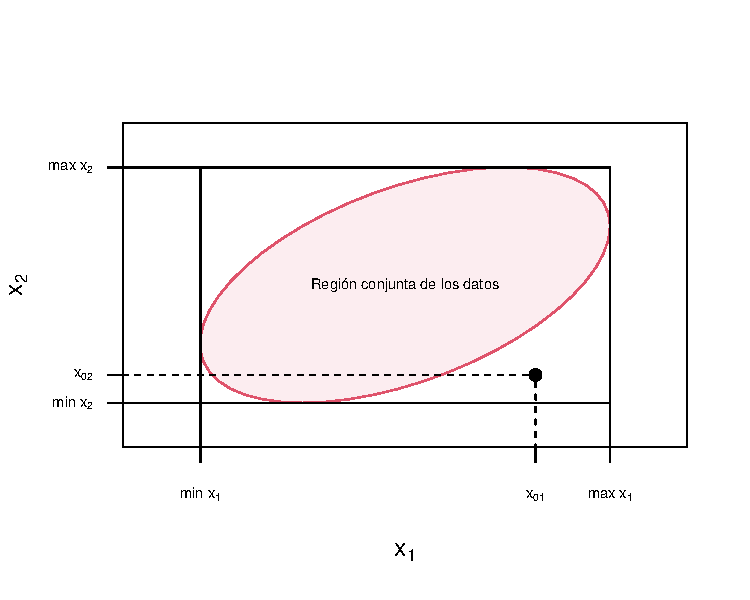
\includegraphics{MLG1_files/figure-latex/extrapolacionOculta-1} 

}

\caption{Ejemplo de extrapolación en regresión múltiple}\label{fig:extrapolacionOculta}
\end{figure}

Determinar la región conjunta de los datos en regresión múltiple no es fácil, lo que hace díficil saber si se está extrapolando a la hora de hacer de una predicción. Por lo tanto, se ha propuesto determinar la región conjunta de los datos a partir del conjunto convexo mínimo que contiene todos los \(n\) datos originales, \((x_{i1}; x_{i2},\ldots,x_{i,p-1})\), para \(i = 1,2,\ldots,n\), como la envolvente de las covariables (RVH). Entonces, si un punto \((x_{01},x_{02}, \ldots,\ldots, x_{0,p-1})\) está dentro o en la frontera de la RVH, una prediccón o una estimación implica interpolación, mientras que si está fuera de la RVH, se está extrapolando.

Una aproximación de la RVH es a través de la matriz \(\boldsymbol H\). El conjunto de puntos \(\boldsymbol x\) que satisfacen, \(\boldsymbol x'(\boldsymbol X'\boldsymbol X)^{-1}\boldsymbol x\leq \max(h_{ii})\), prudcen un elipsoide que encierra todos los puntos dentro de la \(RVH\). Entonces, un punto de predicción \(\boldsymbol x_{0}\) está fuera de la RVH si \(h_{00} > \max{h_{ii}}\), donde:
\[
h_{00} = \boldsymbol x'_{0}(\boldsymbol X'\boldsymbol X)^{-1}\boldsymbol x_{0}.
\]

\rule{\textwidth}{0.4pt}

\hypertarget{bajo-peso-al-nacer---interpolaciuxf3n}{%
\subsubsection*{Bajo peso al nacer - interpolación}\label{bajo-peso-al-nacer---interpolaciuxf3n}}
\addcontentsline{toc}{subsubsection}{Bajo peso al nacer - interpolación}

Suponga que se quiere hacer una predicción para recién nacidos con las características que muestra la Tabla \ref{tab:puntosPrediccion}.

\begin{table}

\caption{\label{tab:puntosPrediccion}Bajo peso al nacer. Punto de predicción.}
\centering
\begin{tabular}[t]{lrrrr}
\toprule
  & 1 & 2 & 3 & 4\\
\midrule
Edad gestacional (semanas) & 34 & 36 & 38 & 46\\
Peso de la madre (kg) & 75 & 50 & 60 & 55\\
\bottomrule
\end{tabular}
\end{table}

La Figura \ref{fig:birthweightExtrapolacion} muestra el gráfico de dispersión de las covariables, donde los puntos rojos indican los valores donde se quieren hacer predicciones. Aquí vemos que en los puntos \(\boldsymbol x_{02}\) y \(\boldsymbol x_{03}\) no estaríamos extrapolando. Pero, es difícil de determinar para los puntos \(\boldsymbol x_{01}\) y \(\boldsymbol x_{04}\). Para esto vamos a calcular las aproximaciones de la RVH y verificar si en estos puntos estaríamos extrapolando.

\begin{figure}

{\centering 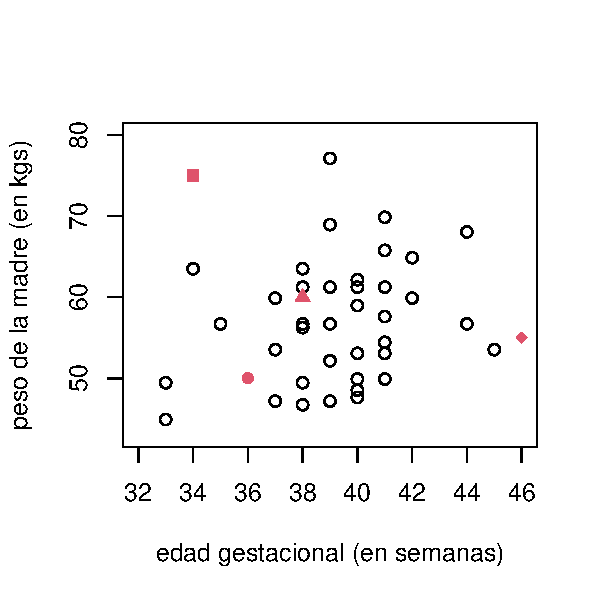
\includegraphics{MLG1_files/figure-latex/birthweightExtrapolacion-1} 

}

\caption{Bajo peso al nacer. Gráfico de dispersion de la edad gestacional y el peso de la madre antes del embarazo. Los puntos donde se quiere hacer predicción están en rojo.}\label{fig:birthweightExtrapolacion}
\end{figure}

\begin{Shaded}
\begin{Highlighting}[]
\NormalTok{newPoints }\OtherTok{=} \FunctionTok{cbind}\NormalTok{(}\AttributeTok{x0=}\FunctionTok{rep}\NormalTok{(}\DecValTok{1}\NormalTok{,}\DecValTok{4}\NormalTok{),}\AttributeTok{x1=}\FunctionTok{c}\NormalTok{(}\DecValTok{34}\NormalTok{,}\DecValTok{36}\NormalTok{,}\DecValTok{38}\NormalTok{,}\DecValTok{46}\NormalTok{),}\AttributeTok{x2=}\FunctionTok{c}\NormalTok{(}\DecValTok{75}\NormalTok{,}\DecValTok{50}\NormalTok{,}\DecValTok{60}\NormalTok{,}\DecValTok{55}\NormalTok{))}
\NormalTok{X }\OtherTok{=} \FunctionTok{model.matrix}\NormalTok{(mod)}
\NormalTok{XtX.inv }\OtherTok{=} \FunctionTok{solve}\NormalTok{(}\FunctionTok{t}\NormalTok{(X)}\SpecialCharTok{\%*\%}\NormalTok{X)}
\NormalTok{h.values }\OtherTok{=} \FunctionTok{hatvalues}\NormalTok{(mod)}
\NormalTok{hmax }\OtherTok{=} \FunctionTok{max}\NormalTok{(h.values)}
\NormalTok{h0 }\OtherTok{=} \FunctionTok{apply}\NormalTok{(newPoints,}\DecValTok{1}\NormalTok{,}\ControlFlowTok{function}\NormalTok{(x)\{}\FunctionTok{t}\NormalTok{(x)}\SpecialCharTok{\%*\%}\NormalTok{XtX.inv}\SpecialCharTok{\%*\%}\NormalTok{x\})}
\NormalTok{h0 }\SpecialCharTok{\textgreater{}}\NormalTok{hmax}
\end{Highlighting}
\end{Shaded}

\begin{verbatim}
## [1]  TRUE FALSE FALSE FALSE
\end{verbatim}

Para la predicción en el punto \(\boldsymbol x_{01}\), tenemos que \(h_{0} = (1, 34, 77)(\boldsymbol X'\boldsymbol X)^{-1}(1, 34, 77)' = 0.3487\) \(>\) \(h_{max} = 0.2276\). Por lo tanto, aquí se estaría extrapolando. Para el resto de punto no hay problemas de extrapolación.

\rule{\textwidth}{0.4pt}

\hypertarget{coeficientes-normalizados-de-regresiuxf3n}{%
\subsubsection{Coeficientes normalizados de regresión}\label{coeficientes-normalizados-de-regresiuxf3n}}

Los coeficientes de regresión están influenciados por las unidades de medida de las covariables. Exactamente las unidades de medida de \(\beta_{j}\) es:
\[
\frac{\mbox{la unidad de medida de }y }{\mbox{la unidad de medida de }x_{j}}.
\]
Dado que, por lo general, las covariables están medidas en unidades diferenes, la comparación de los coeficientes es complicada. En el ejemplo de los datos de los recién nacidos, la edad gestacional está en semanas y el peso de la madre en kilogramos.

Por esta razón, en algunas ocasiones es útil escalar los valores de las covariables y la respuesta para calcular los coeficientes de regresión adimensionales. Hay varias formas de hacer este escalamiento, aquí nos centraremos en el escalamiento de longitud unitaria.

\hypertarget{escalamiento-de-longitud-unitaria}{%
\paragraph{Escalamiento de longitud unitaria}\label{escalamiento-de-longitud-unitaria}}

Una opción es hacer un \textbf{escalamiento de longitud unitaria} a las covariables:
\[
z_{ij} = \frac{x_{ij}-\bar{x}}{\sqrt{S_{jj}}}, i=1,2,\ldots,n \quad j=1,2,\ldots,p-1,
\]
y la variable respuesta:
\[
y_{i}^{*} = \frac{y_{i}-\bar{y}}{\sqrt{SS_{T}}},
\]
donde:
\[
S_{jj} = \sum_{i=1}^{n}(x_{ij} - \bar{x}_{j})^{2}.
\]
Con estas variables transformadas, se puede ajustar el modelo:
\[
y_{i}^{*} = b_{1}z_{i1} + b_{2}z_{i2} + \ldots + b_{p-1}z_{i,p-1} = \boldsymbol z_{i}'\boldsymbol b+ \boldsymbol \varepsilon.
\]
El estimador por MCO es:
\[
\widehat{\boldsymbol b}= (\boldsymbol Z'\boldsymbol Z)^{-1}\boldsymbol Z'\boldsymbol y^{*}.
\]
Note que con este escalamiento, la matriz \((\boldsymbol Z'\boldsymbol Z)\) es igual a la matriz de correlación de las covariables. Esto es:
\[
(\boldsymbol Z'\boldsymbol Z) = \boldsymbol R= \begin{pmatrix}
1 & r_{12} & r_{13} & \ldots & r_{1,p-1} \\
r_{12} & 1 & r_{23} & \ldots & r_{2,p-1} \\
\vdots & \vdots & \vdots & \ddots & \vdots \\
r_{1,p-1} & 1 & r_{2,p-1} & \ldots & 1 \\
\end{pmatrix},
\]
donde \(r_{jk}\) es la correlación entre las covariables \(x_{j}\) y \(x_{k}\). Además, la matriz \(\boldsymbol Z'\boldsymbol y^{*}\) es el vector de correlación entre la variable respuesta y cada covariable. Esto es:
\[
\boldsymbol Z'\boldsymbol y^{*} = (r_{1y},r_{2y},r_{3y},\ldots,r_{p-1,y})',
\]
donde \(r_{jy}\) es la correlación entre la variable respuesta y la covariable \(x_j\).

\rule{\textwidth}{0.4pt}

\hypertarget{bajo-peso-al-nacer---coeficientes-de-regresiuxf3n-con-variables-escaladas}{%
\subsubsection*{Bajo peso al nacer - coeficientes de regresión con variables escaladas}\label{bajo-peso-al-nacer---coeficientes-de-regresiuxf3n-con-variables-escaladas}}
\addcontentsline{toc}{subsubsection}{Bajo peso al nacer - coeficientes de regresión con variables escaladas}

Para estimar los coeficientes de regresión escalados, primero debemos escalar las variables:

\begin{Shaded}
\begin{Highlighting}[]
\NormalTok{y }\OtherTok{=}\NormalTok{ birthweight}\SpecialCharTok{$}\NormalTok{weight}
\NormalTok{Z }\OtherTok{=} \FunctionTok{apply}\NormalTok{(X[,}\SpecialCharTok{{-}}\DecValTok{1}\NormalTok{],}\DecValTok{2}\NormalTok{,}\ControlFlowTok{function}\NormalTok{(x)\{(x}\SpecialCharTok{{-}}\FunctionTok{mean}\NormalTok{(x))}\SpecialCharTok{/}\FunctionTok{sqrt}\NormalTok{(}\FunctionTok{sum}\NormalTok{((x}\SpecialCharTok{{-}}\FunctionTok{mean}\NormalTok{(x))}\SpecialCharTok{\^{}}\DecValTok{2}\NormalTok{))\})}
\NormalTok{ys }\OtherTok{=}\NormalTok{ (y}\SpecialCharTok{{-}}\FunctionTok{mean}\NormalTok{(y))}\SpecialCharTok{/}\FunctionTok{sqrt}\NormalTok{(}\FunctionTok{sum}\NormalTok{((y}\SpecialCharTok{{-}}\FunctionTok{mean}\NormalTok{(y))}\SpecialCharTok{\^{}}\DecValTok{2}\NormalTok{))}
\end{Highlighting}
\end{Shaded}

Ahora procedemos a estimar el modelo con las variables escaladas:

\begin{Shaded}
\begin{Highlighting}[]
\NormalTok{mod.std }\OtherTok{=} \FunctionTok{lm}\NormalTok{(ys}\SpecialCharTok{\textasciitilde{}}\NormalTok{Z}\DecValTok{{-}1}\NormalTok{)}
\FunctionTok{summary}\NormalTok{(mod.std)}
\end{Highlighting}
\end{Shaded}

\begin{verbatim}
## 
## Call:
## lm(formula = ys ~ Z - 1)
## 
## Residuals:
##      Min       1Q   Median       3Q      Max 
## -0.19612 -0.08401  0.01335  0.06533  0.21920 
## 
## Coefficients:
##        Estimate Std. Error t value Pr(>|t|)    
## Zage     0.6986     0.1095   6.379 1.39e-07 ***
## Zmppwt   0.1298     0.1095   1.185    0.243    
## ---
## Signif. codes:  0 '***' 0.001 '**' 0.01 '*' 0.05 '.' 0.1 ' ' 1
## 
## Residual standard error: 0.106 on 40 degrees of freedom
## Multiple R-squared:  0.5503, Adjusted R-squared:  0.5279 
## F-statistic: 24.48 on 2 and 40 DF,  p-value: 1.142e-07
\end{verbatim}

Las estimaciones de los coeficientes son ahora adimensionales y podemos comparar sus magnitudes. Por lo tanto, parece que la covariable edad gestacional es más importante para determinar el peso al nacer que la covariable peso de la madre. Note que, al escalar las variables, los resultados de las pruebas de hipótesis, estimación de \(\sigma^{2}\), y los coeficientes de determinación no se ven alterados.

\rule{\textwidth}{0.4pt}

\hypertarget{multicolinealidad}{%
\subsection{Multicolinealidad}\label{multicolinealidad}}

Un problema que puede afectar enormente el ajuste de un modelo de regresión es la multicolinealidad. Este se presenta cuando hay una dependencia casi lineal entre las covariables.

Recordemos que el estimador por MCO es \(\widehat{\boldsymbol \beta}=(\boldsymbol X'\boldsymbol X)^{-1}\boldsymbol X'\boldsymbol y\). Por lo tanto es necesario que la matriz \(\boldsymbol X'\boldsymbol X\) sea no singular. En caso contrario, no es posible encontrar la inversa y las ecuaciones normales no tendrán una única solución. Cuando sucede esto se debe a que hay al menos una columna de \(\boldsymbol X\) linealmente dependiente.

En regresión se utiliza las palabras multicolinealidad cuando hay una dependencia aproximada en las columnas de \(\boldsymbol X\). Es decir que al menos una covariable puede representarse, de forma aproximada, como una relación lineal de las otras:
\[
x_{ij} \approx c_{0} + c_{1}x_{i1} + \ldots + c_{j-1}x_{i,j-1} + c_{j+1}x_{i,j+1} + \ldots + + c_{p-1}x_{i,p-1},
\]
para \(i=1,\ldots,n\).

Hay que aclarar que la falta de ortogonalidad no es necesariamente un inconveniente, el problema es cuando la relación lineal entre los regresores es casi perfecta, lo que provoca problemas en las inferencias que se hagan. Uno de estos problemas se ilustra a continuación con un ejemplo.

\hypertarget{ejemplo-2}{%
\subsubsection*{ejemplo}\label{ejemplo-2}}
\addcontentsline{toc}{subsubsection}{ejemplo}

Considere el siguiente modelo de regresión:
\[
y_{i} = \beta_{0} + \beta_{1}x_{i1} + \beta_{2}x_{i2} + \varepsilon_{i}, \mbox{ con }\varepsilon_{i}\sim N(0,\sigma^{2}),
\]
y se plantean dos posibles matrices de diseño:
\[
\boldsymbol X_{1} = \begin{pmatrix}
1& 1 \\ 
1 & 5 \\ 
2 & 1 \\ 
2 & 5 \\
\end{pmatrix} \mbox{ y }
\boldsymbol X_{2} = \begin{pmatrix}
1& 1 \\ 
1 & 2 \\ 
2 & 4 \\ 
2 & 5 \\
\end{pmatrix}.
\]
Haciendo el escalamiento de longitud unitaria a las covariables tenemos que:
\[
\boldsymbol Z_{1}'\boldsymbol Z_{1} = \begin{pmatrix}
1 & 0 \\ 0 & 1
\end{pmatrix} \mbox{ y }
\boldsymbol Z_{1}'\boldsymbol Z_{1} = \begin{pmatrix}
1 & 0.95 \\ 0.95 & 1
\end{pmatrix}.
\]
Por lo tanto, la varianza de \(\widehat{\boldsymbol b}\) para ambos casos es:
\[
V(\widehat{\boldsymbol b}_{1}) = \sigma^{2}(\boldsymbol Z_{1}'\boldsymbol Z_{1})^{-1} =  \sigma^{2} \begin{pmatrix}
1 & 0 \\ 0 & 1
\end{pmatrix}^{-1}  = \sigma^{2} \begin{pmatrix}
1 & 0 \\ 0 & 1
\end{pmatrix}.
\]
y
\[
V(\widehat{\boldsymbol b}_{2}) = \sigma^{2}_{0}(\boldsymbol Z_{2}'\boldsymbol Z_{2})^{-1} =  \sigma^{2} \begin{pmatrix}
1 & 0.95 \\ 0.95 & 1
\end{pmatrix}^{-1} = \sigma^{2} \begin{pmatrix}
10 & 9.49 \\ 9.49 & 10
\end{pmatrix}.
\]
Aquí podemos ver que la varianza de \(\widehat{\boldsymbol b}_{2}\) está inflada debido a la alta correlación entre las columnas de \(\boldsymbol X_{2}\). Es 10 veces mayor que la varianza de \(\widehat{\boldsymbol b}_{1}\) (las columnas de \(\boldsymbol X_{1}\) son independientes).

En el ejemplo anterior vemos que los valores de la diagonal de la matriz \((\boldsymbol Z'\boldsymbol Z)^{-1}\) nos indican en cuanto aumenta la varianza de las estimaciones de los coeficientes debido a la multicolinealidad. Por esta razón, estos valores toman el nombre de \textbf{factores de inflación de varianza (VIFs)} y son uno de los indicadores para el diagnostico de este problema.

Se puede demostrar que el VIF de \(\beta_{j}\) se puede calcular como:
\[
\mbox{VIF}_{j} = \frac{1}{1-R^{2}_{j}},
\]
donde \(R^{2}_{j}\) es el coeficiente de determinación obtenido ajustado una regresión de \(x_{j}\) sobre las demás covariables. Si \(x_{j}\) es casi linealmente dependiente de algunos de los otros regresores, entonces \(R^{2}_{j}\) será cercano a uno y el \(VIF_{j}\) será muy alto. Generalmente, un VIF mayor de 10 indica problemas graves de multicolinealidad.

En un capítulo posterior ahondaremos más en este problema.

\rule{\textwidth}{0.4pt}

\hypertarget{bajo-peso-al-nacer---factores-de-inflaciuxf3n-de-varianza}{%
\subsubsection{Bajo peso al nacer - factores de inflación de varianza}\label{bajo-peso-al-nacer---factores-de-inflaciuxf3n-de-varianza}}

En el caso del peso de los recién nacidos, tenemos que los VIFs son:

\begin{Shaded}
\begin{Highlighting}[]
\FunctionTok{library}\NormalTok{(car)}
\FunctionTok{vif}\NormalTok{(mod)}
\end{Highlighting}
\end{Shaded}

\begin{verbatim}
##     age   mppwt 
## 1.06696 1.06696
\end{verbatim}

Lo que nos indica que la varianza de las estimaciones de los coeficientes no se inflan debido a multicolinealidad. Recordemos que la correlación entre las dos covariables no es alta (0.2505155).

\rule{\textwidth}{0.4pt}

\hypertarget{evaluaciuxf3n-de-los-supuestos-del-modelo}{%
\section{Evaluación de los supuestos del modelo}\label{evaluaciuxf3n-de-los-supuestos-del-modelo}}

\rule{\textwidth}{0.4pt}

\hypertarget{ejemplo-1.-datos-de-peso-al-nacer}{%
\subsection*{Ejemplo 1. Datos de peso al nacer}\label{ejemplo-1.-datos-de-peso-al-nacer}}
\addcontentsline{toc}{subsection}{Ejemplo 1. Datos de peso al nacer}

Retomemos la base de datos de bajo peso al nacer (disponible en el campus virtual), y consideremos el siguiente modelo:
\[
\mbox{weight}_{i} = \beta_{0} + \beta_{1}\mbox{age}_{i} + \beta_{2}\mbox{motherage}_{i} + \beta_{3}\mbox{mnocig}_{i} + \beta_{4}\mbox{mppwt}_{i} + \varepsilon_{i},
\]
con \(\varepsilon_{i} \sim N\left(0,\sigma^{2} \right)\) y \(cov(\varepsilon_{j},\varepsilon_{k})=0\), para todo \(j \neq k\).

El ajuste del modelo es:

\begin{Shaded}
\begin{Highlighting}[]
\NormalTok{Birthweight }\OtherTok{=} \FunctionTok{read.csv}\NormalTok{(}\StringTok{\textquotesingle{}birthweight.csv\textquotesingle{}}\NormalTok{)}
\NormalTok{mod.birthweight }\OtherTok{=} \FunctionTok{lm}\NormalTok{(weight }\SpecialCharTok{\textasciitilde{}}\NormalTok{ age }\SpecialCharTok{+}\NormalTok{ motherage }\SpecialCharTok{+}\NormalTok{ mnocig }\SpecialCharTok{+}\NormalTok{ mppwt, }\AttributeTok{data=}\NormalTok{Birthweight)}
\FunctionTok{summary}\NormalTok{(mod.birthweight)}
\end{Highlighting}
\end{Shaded}

\begin{verbatim}
## 
## Call:
## lm(formula = weight ~ age + motherage + mnocig + mppwt, data = Birthweight)
## 
## Residuals:
##      Min       1Q   Median       3Q      Max 
## -0.78765 -0.35948  0.09209  0.35024  0.75018 
## 
## Coefficients:
##              Estimate Std. Error t value Pr(>|t|)    
## (Intercept) -4.104029   1.011723  -4.056 0.000247 ***
## age          0.168027   0.024916   6.744 6.24e-08 ***
## motherage    0.001751   0.012335   0.142 0.887900    
## mnocig      -0.014417   0.005421  -2.660 0.011493 *  
## mppwt        0.014838   0.009530   1.557 0.127966    
## ---
## Signif. codes:  0 '***' 0.001 '**' 0.01 '*' 0.05 '.' 0.1 ' ' 1
## 
## Residual standard error: 0.4073 on 37 degrees of freedom
## Multiple R-squared:  0.627,  Adjusted R-squared:  0.5867 
## F-statistic: 15.55 on 4 and 37 DF,  p-value: 1.5e-07
\end{verbatim}

La edad gestacional y el número de cigarrillos consumidos por la madre tienen efectos signficativos sobre el peso del recién nacido. El primero es un factor de protección, a mayor edad gestacional mayor será el peso del bebé. Mientras que, el consumo de cigarrillos es un factor de riesgo. A mayor consumo, menor peso tendrá el recién nacido. La edad y el peso de la madre, aunque tienen efectos positivos, no son covariables significativas cuando las otras dos covariables ya están incluidas en el modelo.

\rule{\textwidth}{0.4pt}

\hypertarget{ejemplo-2.-ventas-de-helados}{%
\subsection*{Ejemplo 2. Ventas de helados}\label{ejemplo-2.-ventas-de-helados}}
\addcontentsline{toc}{subsection}{Ejemplo 2. Ventas de helados}

La base de datos \texttt{icecream} (del paquete \texttt{orcutt} de R) recopila la siguiente información tomada cada cuatro semanas durante dos años (marzo 1951 a julio 1953):

\begin{itemize}
\tightlist
\item
  \textbf{price}: precio promedio del helado (dolares por bote)
\item
  \textbf{cons}: consumo medio de helado (botes por persona)
\item
  \textbf{temp}: temperatura promedio (en Fahrenheit)
\end{itemize}

La Figura @ref\{fig:icecream\} muestra la relación entre las variables. Aquí podemos observar que a mayor temperatura, el consumo de helado se incrementa. Por otro lado, la relación con el precio no es tan fuerte.

\begin{Shaded}
\begin{Highlighting}[]
\FunctionTok{library}\NormalTok{(orcutt)}
\FunctionTok{data}\NormalTok{(}\StringTok{"icecream"}\NormalTok{)}
\FunctionTok{pairs}\NormalTok{(icecream[,}\FunctionTok{c}\NormalTok{(}\DecValTok{2}\NormalTok{,}\DecValTok{1}\NormalTok{,}\DecValTok{4}\NormalTok{)])}
\end{Highlighting}
\end{Shaded}

\begin{figure}

{\centering 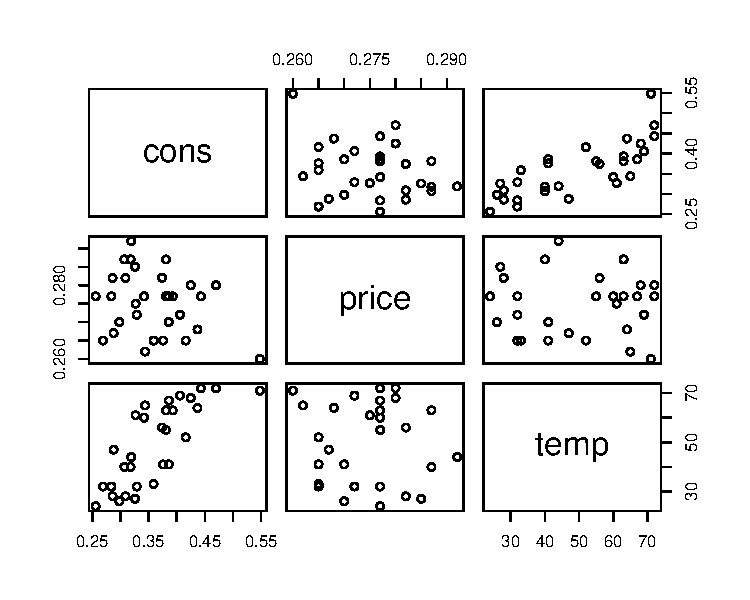
\includegraphics{MLG1_files/figure-latex/Icecream-1} 

}

\caption{\label{fig:icecream} Relación entre las variables de los datos de ventas de helados.}\label{fig:Icecream}
\end{figure}

El objetivo del estudio es explicar el consumo de helado en función del precio y la temperatura. Para esto se propone el siguiente modelo:
\[
\mbox{cons}_{i} = \beta_{0} + \beta_{1}\mbox{price}_{i} + \beta_{2}\mbox{temp}_{i} + \varepsilon_{i},
\]
con \(\varepsilon_{i} \sim N\left(0,\sigma^{2} \right)\) y \(cov(\varepsilon_{j},\varepsilon_{k})=0\), para todo \(j \neq k\).

El resumen del modelo es el siguiente:

\begin{Shaded}
\begin{Highlighting}[]
\NormalTok{  mod.icecream }\OtherTok{=} \FunctionTok{lm}\NormalTok{(cons}\SpecialCharTok{\textasciitilde{}}\NormalTok{price}\SpecialCharTok{+}\NormalTok{temp,}\AttributeTok{data=}\NormalTok{icecream)}
\FunctionTok{summary}\NormalTok{(mod.icecream)}
\end{Highlighting}
\end{Shaded}

\begin{verbatim}
## 
## Call:
## lm(formula = cons ~ price + temp, data = icecream)
## 
## Residuals:
##      Min       1Q   Median       3Q      Max 
## -0.08226 -0.02051  0.00184  0.02272  0.10076 
## 
## Coefficients:
##             Estimate Std. Error t value Pr(>|t|)    
## (Intercept)  0.59655    0.25831   2.309   0.0288 *  
## price       -1.40176    0.92509  -1.515   0.1413    
## temp         0.00303    0.00047   6.448 6.56e-07 ***
## ---
## Signif. codes:  0 '***' 0.001 '**' 0.01 '*' 0.05 '.' 0.1 ' ' 1
## 
## Residual standard error: 0.04132 on 27 degrees of freedom
## Multiple R-squared:  0.6328, Adjusted R-squared:  0.6056 
## F-statistic: 23.27 on 2 and 27 DF,  p-value: 1.336e-06
\end{verbatim}

De aquí podemos concluir que alrededor del 70\% de la variabilidad del consumo de helado está explicado por el modelo propuesto. Además, el efecto de la temperatura sobre el consumo de helado es signficativamente positivo. Aunque la relación con el precio es negativa, esta no es significativa.

\rule{\textwidth}{0.4pt}

\hypertarget{ejemplo-3.-longitud-del-pez-lobina-boca-chica}{%
\subsection*{Ejemplo 3. Longitud del pez lobina boca chica}\label{ejemplo-3.-longitud-del-pez-lobina-boca-chica}}
\addcontentsline{toc}{subsection}{Ejemplo 3. Longitud del pez lobina boca chica}

La base de datos \texttt{wblake} (de la librería \texttt{alr4}) contiene la edad (en años) y longitud (en mm) de 439 peces lobina boca chica del lago West Bearskin en el nordeste de Minnesota en 1999. El objetivo del estudio es determinar los patrones de crecimiento de este tipo de pez.

\begin{Shaded}
\begin{Highlighting}[]
\FunctionTok{library}\NormalTok{(alr4)}
\FunctionTok{data}\NormalTok{(}\StringTok{"wblake"}\NormalTok{)}
\FunctionTok{plot}\NormalTok{(Length}\SpecialCharTok{\textasciitilde{}}\NormalTok{Age,}\AttributeTok{data=}\NormalTok{wblake,}\AttributeTok{xlab=}\StringTok{\textquotesingle{}edad (años)\textquotesingle{}}\NormalTok{,}\AttributeTok{ylab=}\StringTok{\textquotesingle{}longitud (mm)\textquotesingle{}}\NormalTok{)}
\end{Highlighting}
\end{Shaded}

\begin{figure}

{\centering 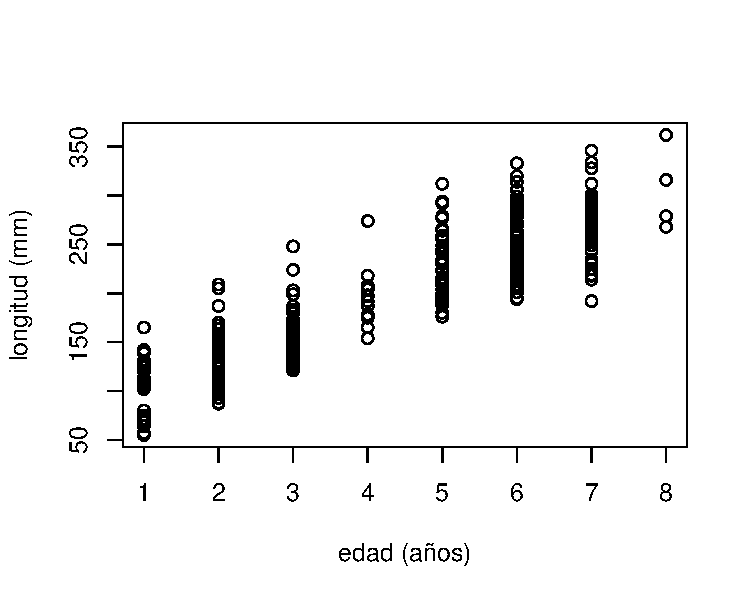
\includegraphics{MLG1_files/figure-latex/bassFig-1} 

}

\caption{\label{fig:bass} Relación entre la edad y la longitud de los peces lobina boca chica.}\label{fig:bassFig}
\end{figure}

La Figura @ref\{fig:bassFig\} muestra que la relación entre estas dos variables se puede aproximar a una recta, por lo cuál se propone el siguiente modelo:
\[
\mbox{length}_{i} = \beta_{0} + \beta_{1}\mbox{age}_{i} + \varepsilon_{i}
\]
con \(\varepsilon_{i} \sim N\left(0,\sigma^{2} \right)\) y \(cov(\varepsilon_{j},\varepsilon_{k})=0\), para todo \(j \neq k\).

El resumen del ajuste es el siguiente:

\begin{Shaded}
\begin{Highlighting}[]
\NormalTok{mod.bass }\OtherTok{=} \FunctionTok{lm}\NormalTok{(Length}\SpecialCharTok{\textasciitilde{}}\NormalTok{Age,}\AttributeTok{data=}\NormalTok{wblake)}
\FunctionTok{summary}\NormalTok{(mod.bass)}
\end{Highlighting}
\end{Shaded}

\begin{verbatim}
## 
## Call:
## lm(formula = Length ~ Age, data = wblake)
## 
## Residuals:
##     Min      1Q  Median      3Q     Max 
## -85.794 -19.499  -4.499  16.177  94.853 
## 
## Coefficients:
##             Estimate Std. Error t value Pr(>|t|)    
## (Intercept)  65.5272     3.1974   20.49   <2e-16 ***
## Age          30.3239     0.6877   44.09   <2e-16 ***
## ---
## Signif. codes:  0 '***' 0.001 '**' 0.01 '*' 0.05 '.' 0.1 ' ' 1
## 
## Residual standard error: 28.65 on 437 degrees of freedom
## Multiple R-squared:  0.8165, Adjusted R-squared:  0.8161 
## F-statistic:  1944 on 1 and 437 DF,  p-value: < 2.2e-16
\end{verbatim}

Estos resultados muestran que la edad del pez tiene un efecto significativamente positivo. Por cada año del pez, la longitud aumenta 30 milimetros en promedio. Adicionalmente, esta covariable explica el 81\% de la variabilidad de la longitud.

\rule{\textwidth}{0.4pt}

La validez de las conclusiones hechas en estos ejemplos descansa en el cumplimiento de los supuestos sobre los errores. Por esta razón, es de gran importancia que tengamos herramientas para evaluar si los datos analizados no muestran ningún alejamiento de los supuestos asumidos.

\hypertarget{supuestos-del-modelo-linea-muxfaltiple}{%
\subsection{Supuestos del modelo linea múltiple}\label{supuestos-del-modelo-linea-muxfaltiple}}

En el modelo de regresión lineal múltiple:
\[
y_{i}=\beta_{0} + \beta_{1} x_{i1}+\beta_{2} x_{i2}+\ldots + \beta_{p-1} x_{i,p-1} +\varepsilon_{i},
\]
asumimos que la relación entre la variable respuesta y las covariables es lineal, al menos de forma aproximada. Además,

\begin{enumerate}
\def\labelenumi{\alph{enumi}.}
\tightlist
\item
  \(E(\varepsilon_{i})=0\), para \(i=1,\ldots,n\),
\item
  \(Var(\varepsilon_{i})=\sigma^{2}\). Homogeneidad de varianza en los errores,
\item
  \(Cov(\varepsilon_{i},\varepsilon_{j})=0\) para todo \(i\neq j\). Los errores están incorrelacionados,
\item
  \(\varepsilon_{i} \sim Normal(0, \sigma^{2})\). Los errores se distribuyen de forma normal.
\end{enumerate}

La importancia de realizar procedimientos para validar los supuestos, radica en que ellos inciden en las cualidades de los estimadores por MCO. En caso de no cumplirse se pueden perder propiedades importantes. Si no se cumple el supuesto (a) se obtienen estimaciones sesgadas. Si no se cumplen (b) y (c) los estimadores MCO pierden la condición de optimalidad. Si no se cumple (d) se pierde eficiencia e imposibilita la aplicación de inferencias basadas en normalidad.

En general, no se puede detectar una violación a los supuestos a partir de estadísticos del ajuste del modelo (\(R^2\), \(F_0\), valores-\(t\), etc). El diagnostico se puede hacer por métodos gráficos y pruebas formales (pruebas de hipótesis). Ambos métodos son complementarios, los gráficos sugieren formas particulares de incumplimiento del supuesto, mientras las pruebas formales evalúan su importancia \citep{behar_validacion_2002}.

\hypertarget{efectos-del-incumplimiento-de-los-supuestos}{%
\subsection{Efectos del incumplimiento de los supuestos}\label{efectos-del-incumplimiento-de-los-supuestos}}

\hypertarget{sesgo-por-omisiuxf3n-de-variables-relevantes}{%
\subsubsection{Sesgo por omisión de variables relevantes}\label{sesgo-por-omisiuxf3n-de-variables-relevantes}}

Si \(E(\boldsymbol \varepsilon) = \boldsymbol 0\), entonces \(E(\boldsymbol y| \boldsymbol X) = \boldsymbol X\boldsymbol \beta\), y el estimador por MCO es insesgado. Sin embargo, si omitimos variables relevantes dentro del modelo las estimaciones serán sesgadas. Para ver esto, supongamos que el modelo generador de los datos es:
\[
\boldsymbol y= \boldsymbol X\boldsymbol \beta+ \boldsymbol \varepsilon=  \boldsymbol X_{1}\boldsymbol \beta_{1} + \boldsymbol X_{2}\boldsymbol \beta_{2} + \boldsymbol \varepsilon,
\]
donde las columnas de la matriz \(n\times p\) de covariables \(\boldsymbol X\) está divida en dos submatrices \(\boldsymbol X_{1}\) y \(\boldsymbol X_{2}\) de dimensiones \(n \times (p-r)\) y \(n\times r\), respectivamente. Además, asumimos que \(\boldsymbol \varepsilon\sim N(\boldsymbol 0, \sigma^{2}\boldsymbol I_{n})\).

Ahora, consideramos estimar el siguiente modelo:
\[
\boldsymbol y= \boldsymbol X_{1}\boldsymbol \beta_{1} + \boldsymbol \varepsilon^{*},
\]
es decir estamos omitiendo las covariables contenidas en \(\boldsymbol X_{2}\). El estimador de \(\boldsymbol \beta_{1}\) es:
\[
\widehat{\boldsymbol \beta}_{1} = (\boldsymbol X_{1}'\boldsymbol X_{1})^{-1}\boldsymbol X_{1}'\boldsymbol y,
\]
y el estimador de \(\sigma^{2}\) es:
\[
\widehat{\sigma}^{2}_{1} = \frac{\boldsymbol y'(\boldsymbol I_{n} - \boldsymbol H_{1})\boldsymbol y}{n-(p-r)}, \mbox{ donde }\boldsymbol H_{1} = \boldsymbol X_{1}(\boldsymbol X_{1}'\boldsymbol X_{1})^{-1}\boldsymbol X_{1}'.
\]
El valor esperado de \(\widehat{\boldsymbol \beta}_{1}\) es:
\begin{equation}
\begin{split}
E(\widehat{\boldsymbol \beta}_{1}) &= E\left[(\boldsymbol X_{1}'\boldsymbol X_{1})^{-1}\boldsymbol X_{1}'\boldsymbol y\right] = (\boldsymbol X_{1}'\boldsymbol X_{1})^{-1}\boldsymbol X_{1}'E(\boldsymbol y) \\
&= (\boldsymbol X_{1}'\boldsymbol X_{1})^{-1}\boldsymbol X_{1}'E(\boldsymbol X_{1}\boldsymbol \beta_{1} + \boldsymbol X_{2}\boldsymbol \beta_{2} + \boldsymbol \varepsilon) = \boldsymbol \beta_{1} +  (\boldsymbol X_{1}'\boldsymbol X_{1})^{-1}\boldsymbol X_{1}'\boldsymbol X_{2}\boldsymbol \beta_{2}.
\end{split}
\nonumber
\end{equation}
Evidentemente, el sesgo de \(\widehat{\boldsymbol \beta}_{1}\) depende de la magnitud de \(\boldsymbol \beta_{2}\). Entre más importante sean los efectos asociados a las covariables omitidas \((\boldsymbol \beta_{2})\), mayor será el sesgo. Si las columnas de \(\boldsymbol X_{1}\) son ortogonales de las columnas de \(\boldsymbol X_{2}\), tenemos que \(\boldsymbol X_{1}'\boldsymbol X_{2} = \boldsymbol 0\). Así que, en este caso particular, \(\widehat{\boldsymbol \beta}_{1}\) es insesgado (así omitamos las covariables en \(\boldsymbol X_{2}\)).

El valor esperado de \(\widehat{\sigma}^{2}_{1}\) es:
\[
E(\widehat{\sigma}^{2}_{1}) = \sigma^{2} + \frac{\boldsymbol \beta_{2}'\boldsymbol X'_{2}(\boldsymbol I_{n} - \boldsymbol H_{1})\boldsymbol X_{2}\boldsymbol \beta_{2}}{n-(p-r)}.
\]
Dado que \((\boldsymbol I- \boldsymbol H_{1})\) es idempotente y, por lo tanto, positiva semi-definida, entonces \(E(\widehat{\sigma}_{1}^{2}) > \sigma^{2}\). Lo que quiere decir que \(\widehat{\sigma}^{2}_{1}\) es un estimador sesgado de \(\sigma^{2}\).

Ahora veamos el efecto de omitir covariables relevantes sobre las predicciones de \(y\) en el punto \(\boldsymbol x_{0} = (\boldsymbol x_{01}', \boldsymbol x_{02}')'\). Tenemos que:
\[
\widehat{\boldsymbol y}_{0} = \boldsymbol x_{01}'\widehat{\boldsymbol \beta}_{1} = \boldsymbol x_{01}'(\boldsymbol X_{1}'\boldsymbol X_{1})^{-1}\boldsymbol X_{1}'\boldsymbol y.
\]
El valor esperado de \(\widehat{\boldsymbol y}_{0}\) es:
\[
E(\widehat{\boldsymbol y}_{0}) = \boldsymbol x_{01}'E(\widehat{\boldsymbol \beta}_{1}) = \boldsymbol x_{01}'\left[ \boldsymbol \beta_{1} +  (\boldsymbol X_{1}'\boldsymbol X_{1})^{-1}\boldsymbol X_{1}'\boldsymbol X_{2}\boldsymbol \beta_{2} \right]. 
\]
Por lo tanto las predicciones también son sesgadas, \(E(\widehat{\boldsymbol y}_{0}) \neq \boldsymbol x_{01}'\boldsymbol \beta_{1} + \boldsymbol x_{02}'\boldsymbol \beta_{2}\).

\hypertarget{incorrecta-matriz-de-varianzas-de-los-errores}{%
\subsubsection{Incorrecta matriz de varianzas de los errores}\label{incorrecta-matriz-de-varianzas-de-los-errores}}

Cuando \(V(\boldsymbol \varepsilon) = \sigma^{2}\boldsymbol V\), pero asumimos erroneamente que \(V(\boldsymbol \varepsilon) = \sigma^{2}\boldsymbol I_{n}\), el estimador \(\widehat{\boldsymbol \beta}\) sigue siendo insesgado. Pero, tenemos que:
\begin{equation}
\begin{split}
V(\widehat{\boldsymbol \beta}) &= V\left[ (\boldsymbol X'\boldsymbol X)^{-1}\boldsymbol X'\boldsymbol y\right] = (\boldsymbol X'\boldsymbol X)^{-1}\boldsymbol X'V(\boldsymbol y)\boldsymbol X(\boldsymbol X'\boldsymbol X)^{-1} \\
&= \sigma^{2}(\boldsymbol X'\boldsymbol X)^{-1}\boldsymbol X'\boldsymbol V\boldsymbol X(\boldsymbol X'\boldsymbol X)^{-1},
\end{split}
\nonumber
\end{equation}
es, generalmente, diferente de \(\sigma^{2}(\boldsymbol X'\boldsymbol X)^{-1}\) (la varianza que asumimos como cierta). Igualmente, el estimador por MCO pierde su condición de optimalidad. Es decir, deja de ser el mejor estimador lineal insesgado.

El estimador de \(\sigma^{2}\) es sesgado:
\[
E(\widehat{\sigma}^{2}) = \frac{\sigma^{2}}{n-p}E\left[\boldsymbol y'(\boldsymbol I_{n} - \boldsymbol H)\boldsymbol y\right] = \frac{\sigma^{2}}{n-p} \mbox{tr}\left[ \boldsymbol V(\boldsymbol I_{n}-\boldsymbol H)\right].
\]
Las predicciones son insesgadas, pero:
\[
V(\widehat{y}_{0}) = V(\boldsymbol x_{0}'\widehat{\boldsymbol \beta}) = \sigma^{2}\boldsymbol x_{0}'(\boldsymbol X'\boldsymbol X)^{-1}\boldsymbol X'\boldsymbol V\boldsymbol X(\boldsymbol X'\boldsymbol X)^{-1} \boldsymbol x_{0},
\]
que es diferente de \(\sigma^{2}\boldsymbol x_{0}'(\boldsymbol X'\boldsymbol X)^{-1}\boldsymbol x_{0}\) (la varianza que asumimos como cierta).

Cuando \(\boldsymbol V\) es una matriz diagonal:
\[
\boldsymbol V= \begin{pmatrix}
v_{11} & 0 & 0 & \ldots & 0 \\
0 & v_{22} & 0 & \ldots & 0 \\
0 & 0 & v_{33} & \ldots & 0 \\
\vdots & \vdots & \vdots & \ddots & \vdots \\
0 & 0 & 0 & \ldots & v_{nn}
\end{pmatrix},
\]
tenemos que hay \textbf{heterocedasticidad}. Cada error tiene una varianza diferente \(V(\varepsilon_{j})=\sigma^{2}v_{jj}\), pero están incorrelacionados. Si los valores fuera de la diagonal de \(\boldsymbol V\) son diferentes de cero, entonces los errores están correlacionados.

La correlación de los errores puede esperarse en algunas situaciones. Por ejemplo, si las observaciones son tomadas en el tiempo puede presentarse correlación temporal. En situaciones en las que se pueda garantizar que las observaciones \((y_{1},y_{2},\ldots,y_{n})\) constituyen una muestra aleatoria, no existirá correlación entre los errores, es decir, que es posible controlar este aspecto, algunas ocasiones, controlando el procedimiento de selección de la muestra.

\hypertarget{distribuciuxf3n-no-normal-de-los-errores}{%
\subsubsection{Distribución no normal de los errores}\label{distribuciuxf3n-no-normal-de-los-errores}}

La normalidad de los errores permite la estimación por intervalos de confianza no sólo para los coeficientes de regresión, sino también para la predicción. Igualmente, permite el planteamiento de pruebas de hipótesis sobre los parámetros del modelo. Cuando los errores no son normales, estas inferencias no son exactas y pueden llegar a ser inválidas.

Sin embargo, el teorema central del límite asegura que, bajo ciertas condiciones muy amplias, la inferencias basadas en el estimador de mínimos cuadrados son aproximadamente válidas si el tamaño de muestra es suficientemente grande. Esto significa que los niveles de las pruebas y cobertura de los intervalos de confianza son aproximadamente correctos.

De la misma forma, los efectos negativos de la no normalidad dependen de que tan alejados estamos de la normalidad. Si la distribución de los errores es parecida a la normal (por ejemplo, \(t\)-Student), los efectos negativos no son considerables.

\hypertarget{residuos-del-modelo}{%
\subsection{Residuos del modelo}\label{residuos-del-modelo}}

Los residuos están definidos como:
\[
e_{i} = y_{i}- \widehat{y}_{i}, \mbox{ en forma matricial }\boldsymbol e= \boldsymbol y- \widehat{\boldsymbol y}= (\boldsymbol I_{n} - \boldsymbol H)\boldsymbol y.
\]
Los residuos representan las desviaciones entre las observaciones y el ajuste. Además, estos son combinaciones lineales de los errores:
\[
\boldsymbol e= (\boldsymbol I_{n} - \boldsymbol H)(\boldsymbol X\boldsymbol \beta+\boldsymbol \varepsilon) = (\boldsymbol I_{n} - \boldsymbol H)\boldsymbol \varepsilon.
\]
Por lo tanto toda desviación de las premisas de los errores se debe reflejar en los residuales. Si \(\boldsymbol \varepsilon\sim N(\boldsymbol 0,\sigma^{2}\boldsymbol I_{n})\), entonces:
\[
\boldsymbol e\sim N \left[ \boldsymbol 0, \sigma^{2}(\boldsymbol I_{n} - \boldsymbol H)  \right].
\]
De aquí tenemos que \(V(e_{i}) = (1-h_{ii})\sigma^{2}\) y \(Cov(e_{i},e_{j}) = - h_{ij}\sigma^{2}\), para todo \(i \neq j\). Lo que indica que, aún cuando los errores sean homogéneos en varianza e incorrelacionados, no implica que los residuos lo sean también. Note que los residuos asociados a puntos alejados del centro de los datos tienen menor varianza. Lo que hace difícil detectar violaciones.

Cuando \(n\) es grande comparado con el número de parámetros en el modelo, los residuos si reflejan a los errores en cuanto al comportamiento de su varianza y correlación. Esto es porque \(|h_{ij}| \leq 1\), \(\sum_{i=1}^{n}h_{ii} = n-p\), y \(\sum_{i=1}^{n}h_{ij}=\sum_{j=1}^{n}h_{ij}=1\). Por lo tanto, cuando \(n\rightarrow \infty\), \(V(e_{i}) = \sigma^{2}\) y \(Cov(e_{i},e_{j}) = 0\).

\hypertarget{residuos-estudentizados}{%
\subsubsection{Residuos estudentizados}\label{residuos-estudentizados}}

Para evitar el inconveniente de la varianza no constante de los residuos, es preferible utilizar los \textbf{residuos estudentizados}:
\[
r_{i} = \frac{e_{i}}{\sqrt{\hat{\sigma}^{2}(1-h_{ii})}}, \qquad i=1,2,\ldots,n.
\]
Entonces, \(r_{i}\) tiene varianza constante (\(V(r_{i})=1\)) independiente del lugar de \(\boldsymbol x_{i}\).

\hypertarget{residuos-press-y-r-student}{%
\subsubsection{Residuos PRESS y R-student}\label{residuos-press-y-r-student}}

Como veremos más adelante, los residuos estudentizados se pueden utilizar detectar puntos atípicos. El problema es que si la \(i\)-ésima observación es bastante inusual, el ajuste del modelo puede estar muy influenciado por esta observación. Lo que puede producir un residuo pequeño. Por esta razón, también se pueden calcular los residuos de predicción (PRESS). Estos se calculan de la siguiente forma:
\[
e_{(i)} = y_{i} - \widehat{y}_{(i)}, \mbox{ para }i=1,\ldots,n,
\]
donde \(\widehat{y}_{(i)}\) es el valor ajustado para la \(i\)-ésima observación usando todas las observaciones excepto la \(i\)-ésima. Esto implicaría que para calcular los residuos PRESS es necesario ajustar \(n\) veces el modelo. Sin embargo, esto no es así, ya que se puede demostrar que:
\[
e_{(i)} = \frac{e_{i}}{1-h_{ii}}.
\]
La varianza de los residuos PRESS es:
\[
V(e_{(i)}) = V\left( \frac{e_{i}}{1-h_{ii}} \right) = \frac{1}{(1-h_{ii})^{2}}V(e_{i}) = \frac{1}{(1-h_{ii})^{2}} [\sigma^{2}(1-h_{ii})] = \frac{\sigma^{2}}{(1-h_{ii})}.
\]
Si estudentizamos los residuos PRESS obtenemos los \textbf{residuos R-Student}:
\[
t_{i} = \frac{e_{i}}{\sqrt{\widehat{\sigma}^{2}_{(i)}(1-h_{ii})}},
\]
donde \(\widehat{\sigma}^{2}_{(i)}\) es la estimación de \(\sigma\) usando todas las observaciones excepto la \(i\)-ésima. Se puede demostrar que:
\[
\widehat{\sigma}^{2}_{(i)} = \frac{(n-p)\widehat{\sigma}^{2} - e^{2}_{i}/(1-h_{ii})}{n-p-1}.
\]

\hypertarget{evaluaciuxf3n-del-cumplimiento-de-los-supuestos}{%
\subsection{Evaluación del cumplimiento de los supuestos}\label{evaluaciuxf3n-del-cumplimiento-de-los-supuestos}}

En esta sección mostramos la evaluación de los supuestos a través del análisis de los residuos del ajuste (ya sean los residuos estudentizados o los R-Student) usando gráficos y pruebas de hipótesis.

\hypertarget{gruxe1ficos-de-residuos}{%
\subsubsection{Gráficos de residuos}\label{gruxe1ficos-de-residuos}}

Un gráfico de los residuos es una forma efectiva de investigar posibles alejamientos de los supuestos. Generalmente, se grafican los residuos estudentizados \((r_{i})\) contra los valores ajustados \(\widehat{y}_{i}\) (o contra alguna de las covariables \(x_{ij}\)). Este tipo de gráfico es de gran ayuda para detectar la correcta especificación del modelo y homocedasticidad. Algunos patrones de residuos se pueden observar en la Figura \ref{fig:PatronesResiduos}.

\begin{figure}

{\centering 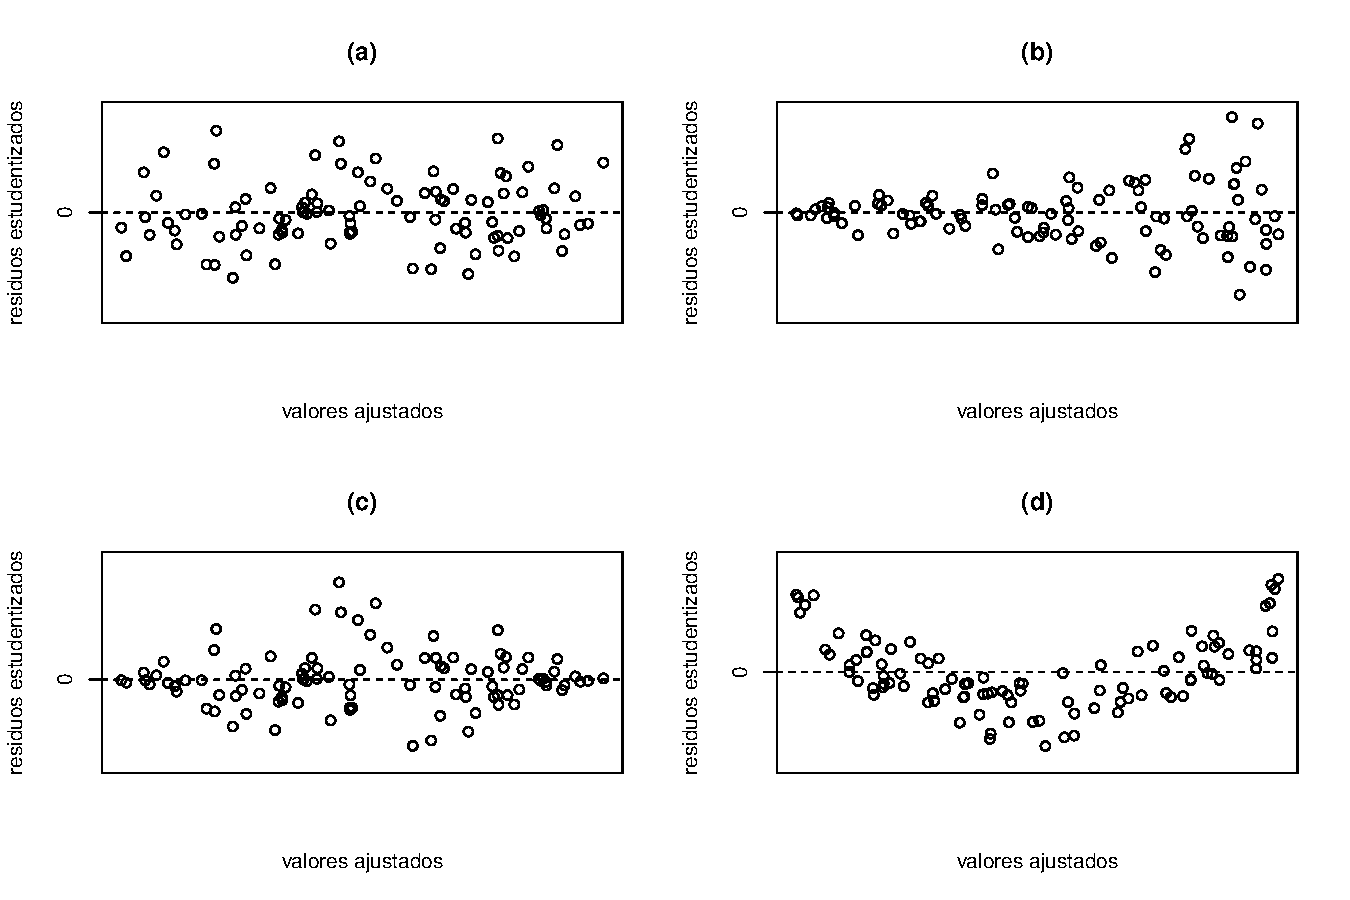
\includegraphics{MLG1_files/figure-latex/PatronesResiduos-1} 

}

\caption{Ejemplos de posibles patrones de residuos}\label{fig:PatronesResiduos}
\end{figure}

La Figura \ref{fig:PatronesResiduos}(a) muestra que los residuos se encuentran alrededor de cero y no se observa ningún patrón claro. Esto es un indicio que el modelo está bien especificado y hay homocedasticidad. En la Figura \ref{fig:PatronesResiduos}(b) vemos que los residuos están alrededor de cero pero la variabilidad crece a medida que los valores ajustados aumenta. Esto es un indicador de heterocedasticidad. La Figura \ref{fig:PatronesResiduos}(c) también muestra un patrón de heterocedasticidad, la variabilidad aumenta hasta cierto punto y luego decrece. En la Figura \ref{fig:PatronesResiduos}(d) observamos que los residuos no fluctuan alrededor de cero, sino que siguen una curva. Esto nos que la relación entre la variable respuesta y las covariables no es lineal.

\begin{figure}

{\centering 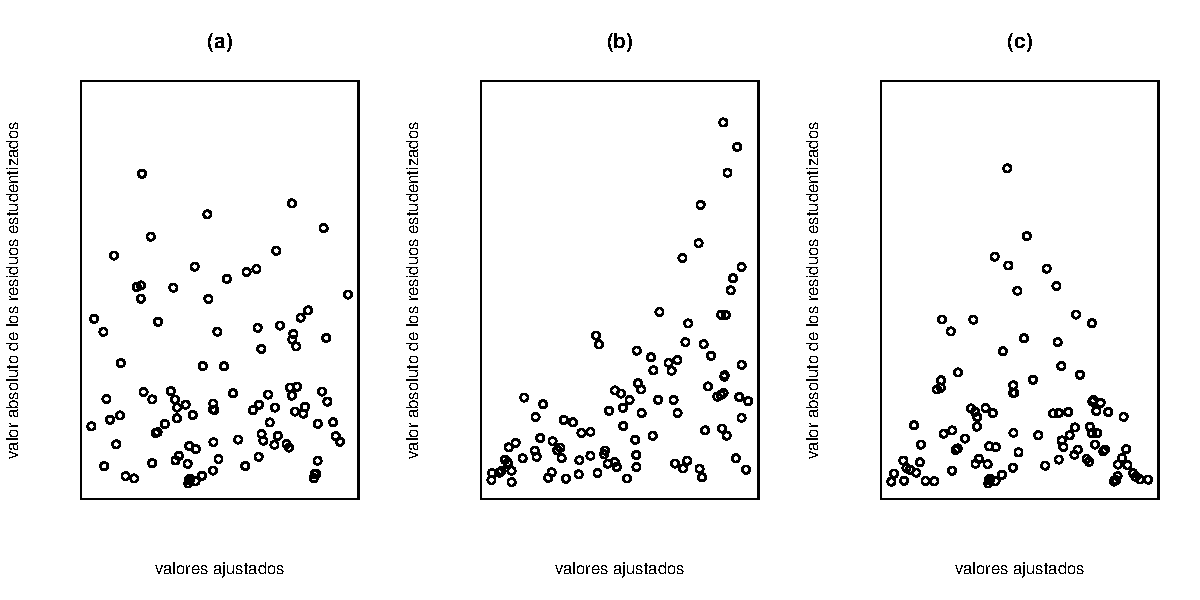
\includegraphics{MLG1_files/figure-latex/patronesResiduos2-1} 

}

\caption{Ejemplos de posibles patrones de residuos (graficando el valor absoluto de los residuos).}\label{fig:patronesResiduos2}
\end{figure}

Adicionalmente, para detectar más facilmente heterocedasticidad, se pueden graficar el valor absoluto de los residuos estudentizados (o al cuadrado) contra los valores ajustados (o las covariables). La Figura \ref{fig:patronesResiduos2} muestra los mismos patrones pero graficando los residuos en valor absoluto. En las Figuras \ref{fig:patronesResiduos2}(b-c) se evidencia claramente la heterocedasticidad.

\rule{\textwidth}{0.4pt}

\hypertarget{bajo-peso-al-nacer---gruxe1fico-de-residuos}{%
\paragraph*{Bajo peso al nacer - gráfico de residuos}\label{bajo-peso-al-nacer---gruxe1fico-de-residuos}}
\addcontentsline{toc}{paragraph}{Bajo peso al nacer - gráfico de residuos}

Para el modelo ajustado para los datos de peso al nacer, el gráfico de los residuos contra los valores ajustados se obtienen de la siguiente forma:

\begin{Shaded}
\begin{Highlighting}[]
\FunctionTok{library}\NormalTok{(MASS)}
\NormalTok{res.stud.birthweight }\OtherTok{=} \FunctionTok{studres}\NormalTok{(mod.birthweight)}
\NormalTok{mod.fit.birthweight }\OtherTok{=}\NormalTok{ mod.birthweight}\SpecialCharTok{$}\NormalTok{fitted.values}
\FunctionTok{par}\NormalTok{(}\AttributeTok{mfrow=}\FunctionTok{c}\NormalTok{(}\DecValTok{1}\NormalTok{,}\DecValTok{2}\NormalTok{))}
\FunctionTok{plot}\NormalTok{(mod.fit.birthweight,res.stud.birthweight, }\AttributeTok{ylab=}\StringTok{\textquotesingle{}residuos estudentizados\textquotesingle{}}\NormalTok{,}
     \AttributeTok{xlab=}\StringTok{\textquotesingle{}valores ajustados\textquotesingle{}}\NormalTok{,}\AttributeTok{main=}\StringTok{\textquotesingle{}(a)\textquotesingle{}}\NormalTok{)}
\FunctionTok{abline}\NormalTok{(}\AttributeTok{h=}\DecValTok{0}\NormalTok{,}\AttributeTok{lty=}\DecValTok{2}\NormalTok{)}
\FunctionTok{lines}\NormalTok{(}\FunctionTok{lowess}\NormalTok{(res.stud.birthweight}\SpecialCharTok{\textasciitilde{}}\NormalTok{mod.fit.birthweight), }\AttributeTok{col =} \DecValTok{2}\NormalTok{)}
\FunctionTok{plot}\NormalTok{(mod.fit.birthweight,}\FunctionTok{abs}\NormalTok{(res.stud.birthweight), }
     \AttributeTok{ylab=}\StringTok{\textquotesingle{}valor absoluto de los residuos estudentizados\textquotesingle{}}\NormalTok{,}
     \AttributeTok{xlab=}\StringTok{\textquotesingle{}valores ajustados\textquotesingle{}}\NormalTok{,}\AttributeTok{main=}\StringTok{\textquotesingle{}(b)\textquotesingle{}}\NormalTok{)}
\FunctionTok{lines}\NormalTok{(}\FunctionTok{lowess}\NormalTok{(}\FunctionTok{abs}\NormalTok{(res.stud.birthweight)}\SpecialCharTok{\textasciitilde{}}\NormalTok{mod.fit.birthweight), }\AttributeTok{col =} \DecValTok{2}\NormalTok{)}
\end{Highlighting}
\end{Shaded}

\begin{figure}

{\centering 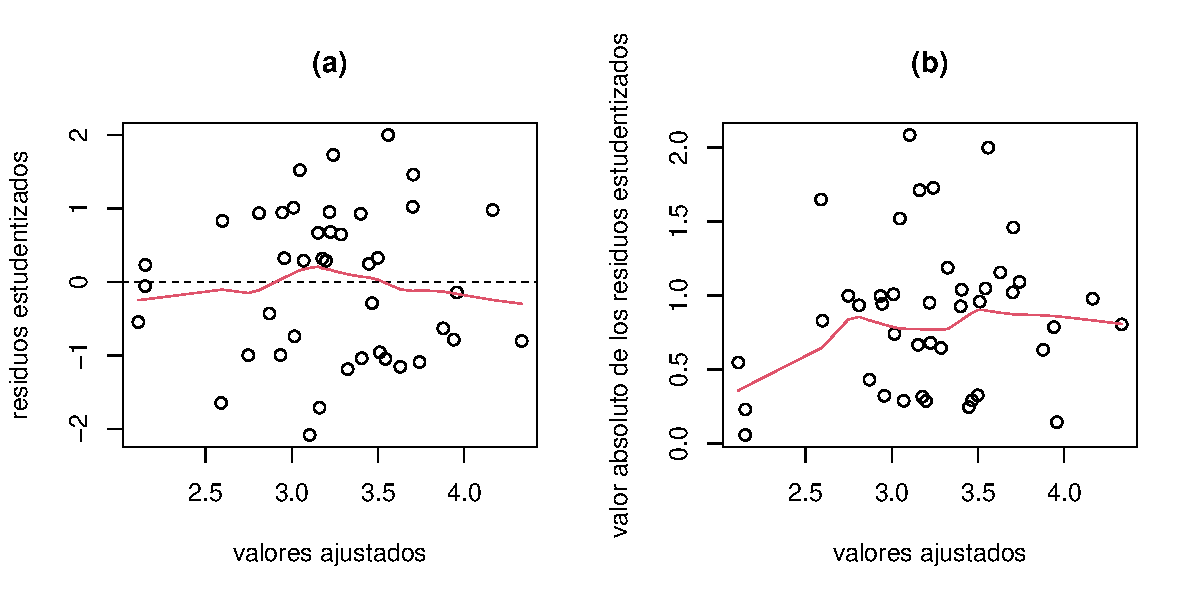
\includegraphics{MLG1_files/figure-latex/residuosBWdata-1} 

}

\caption{Datos de peso al nacer. Gráfico de los residuos estudentizados contra los valores ajustados.}\label{fig:residuosBWdata}
\end{figure}

La Figura \ref{fig:residuosBWdata}(a) muestra que los residuos están alrededor de cero sin mostrar ningún patrón. Note que este gráfico es similar a la Figura \ref{fig:PatronesResiduos}(a). La línea roja es una suaviación LOWESS (Locally weighted scatterplot smoothing, más detalle ver Apéndice A.5 de \citet{weisberg_applied_2014}). Estas suavizaciones permiten ver fácilmente patrones de comportamiento. Aquí vemos que la suavización está cerca de la recta en cero sin mostrar ninguna tendencia o curvatura muy marcada. Por lo tanto, podemos afirmar que la relación entre el peso del recién nacido y las covariables propuesta es lineal. Además, no se observa un problema notorio de heterocedasticidad en ninguno de los dos gráficos de residuos.

\rule{\textwidth}{0.4pt}

\hypertarget{gruxe1ficos-de-residuos-parciales}{%
\subsubsection{Gráficos de residuos parciales}\label{gruxe1ficos-de-residuos-parciales}}

Los gráficos de residuos parciales permiten estudiar el efecto marginal de una covariable sobre la respuesta condicionado a que los demás regresores ya están en el modelo. En caso que el gráfico de los residuos muestre posibles curvaturas (por ejemplo, Figura \ref{fig:PatronesResiduos}(d)), los residuos parciales permiten verificar si estas se presentan debido a una covariable especifica.

Considere el modelo:
\[
y_{i} = \beta_{0} +\beta_{1}x_{i1}+\beta_{2}x_{i2} + \ldots + \beta_{p-1}x_{i,p-1} + \varepsilon_{i}.
\]
Para calcular los residuos parciales, primero estimamos los parámetros \((\widehat{\beta}_{1},\ldots,\widehat{\beta}_{p-1})\) y los residuos ordinarios \((e_{1},\ldots,e_{n})\). Luego, los residuos parciales para la covariable \(x_{j}\) se obtienen de la siguiente forma:
\[
e^{*}_{i}(y|x_{j}) = e_{i} - \widehat{\beta}_{j}x_{ij}.
\]
El gráfico de residuos parciales para la covariable \(x_{j}\) se obtiene graficando \(e^{*}_{i}(y|x_{j})\) contra \(x_{j}\). Si la covariable \(x_{j}\) entra al modelo linealmente, entonces el gráfico de residuos parciales debe mostrar una tendencia lineal. Por el contrario, si se observa una curva, \(x_{j}\) no entra al modelo de forma lineal.

\rule{\textwidth}{0.4pt}

\hypertarget{bajo-peso-al-nacer---gruxe1fico-de-residuos-parciales}{%
\paragraph*{Bajo peso al nacer - gráfico de residuos parciales}\label{bajo-peso-al-nacer---gruxe1fico-de-residuos-parciales}}
\addcontentsline{toc}{paragraph}{Bajo peso al nacer - gráfico de residuos parciales}

El gráfico de residuos parciales se obtiene así:

\begin{Shaded}
\begin{Highlighting}[]
\FunctionTok{library}\NormalTok{(car)}
\FunctionTok{par}\NormalTok{(}\AttributeTok{mfrow=}\FunctionTok{c}\NormalTok{(}\DecValTok{2}\NormalTok{,}\DecValTok{2}\NormalTok{))}
\FunctionTok{crPlots}\NormalTok{(mod.birthweight,}\StringTok{\textquotesingle{}age\textquotesingle{}}\NormalTok{,}\AttributeTok{xlab=}\StringTok{\textquotesingle{}edad gestacional\textquotesingle{}}\NormalTok{)}
\FunctionTok{crPlots}\NormalTok{(mod.birthweight,}\StringTok{\textquotesingle{}motherage\textquotesingle{}}\NormalTok{,}\AttributeTok{xlab=}\StringTok{\textquotesingle{}edad de la madre\textquotesingle{}}\NormalTok{)}
\FunctionTok{crPlots}\NormalTok{(mod.birthweight,}\StringTok{\textquotesingle{}mnocig\textquotesingle{}}\NormalTok{,}\AttributeTok{xlab=}\StringTok{\textquotesingle{}número de cigarrillos por mes\textquotesingle{}}\NormalTok{)}
\FunctionTok{crPlots}\NormalTok{(mod.birthweight,}\StringTok{\textquotesingle{}mppwt\textquotesingle{}}\NormalTok{,}\AttributeTok{xlab=}\StringTok{\textquotesingle{}peso de la madre\textquotesingle{}}\NormalTok{)}
\end{Highlighting}
\end{Shaded}

\begin{figure}

{\centering 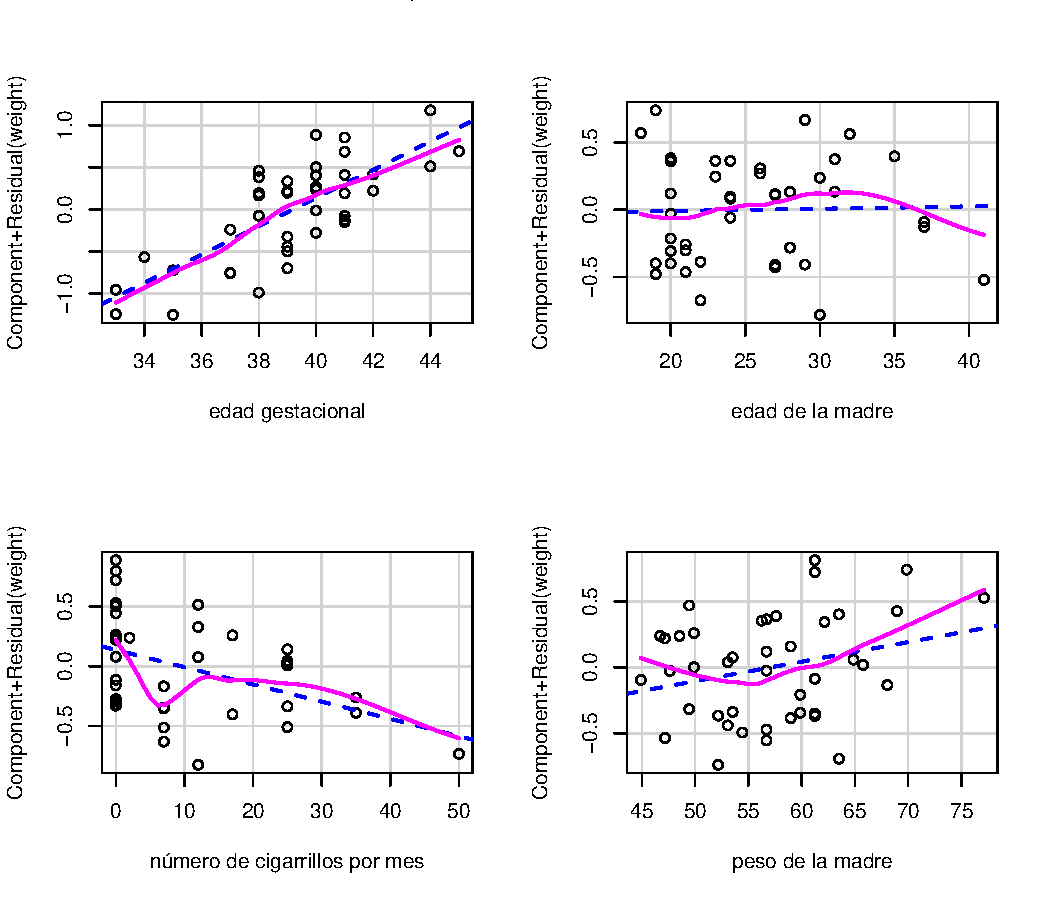
\includegraphics{MLG1_files/figure-latex/residuosBWdata2-1} 

}

\caption{Datos de peso al nacer. Gráfico de los residuos parciales para cada covariable.}\label{fig:residuosBWdata2}
\end{figure}

Igual que en el gráfico de residuos, los residuos parciales no muestran tendencias no lineales muy marcada. Por lo que se puede asumir que la relación entre el peso al nacer y las covariables es lineal.

\rule{\textwidth}{0.4pt}

\hypertarget{gruxe1ficos-de-normalidad}{%
\subsubsection{Gráficos de normalidad}\label{gruxe1ficos-de-normalidad}}

Los gráficos cuantil-cuantil (qqplot) comparan los cuantiles muestrales contra los cuantiles que se esperarían con la distribución de probabilidad asumida para los datos (cuantiles teóricos). En el caso de regresión lineal, estamos asumiendo que los errores del modelo siguen una distribución normal. Por lo tanto, debemos comparar los cuartiles muestrales de los residuos con los cuartiles teóricos que se esperarían bajo una distribución normal.

Sea \((x_{1},x_{2},\ldots,x_{n})\) una muestra aleatoría de la variable \(X\) con función de distribución desconocida \(F_{X}(x)\), y sean \((x_{[1]},x_{[2]},\ldots,x_{[n]})\) los estadísticos de orden (observaciones ordenadas de forma creciente). La función empirica de distribución es:
\[
S_{n}(x_{[i]}) = \frac{i}{n} = \frac{\mbox{\# de observaciones }\leq x_{[i]}}{n}.
\]
Si asumimos que \(X\sim N(0,1)\), entonces los puntos \((x_{[i]},\Phi^{-1}\left\{S_{n}(x_{[i]})\right\})\), donde \(\Phi^{-1}()\) es la inversa de la función acumulativa de una normal estándar, deben seguir aproximadamente una línea recta.

La Figura \ref{fig:qqplots} muestra diferentes patrones de gráficos de normalidad para datos generados a partir de tres distribuciones diferentes: normal estándar (derecha), exponencial con \(\lambda=1\) (centro), y \(t\)-Student con 2 grados de libertad (derecha). Aquí vemos que para los datos normales, los cuantiles muestrales y teóricos siguen aproximadamente la linea recta de referencia. Mientras que en los otros dos casos, los puntos se alejan en los extremos. En el caso de los datos exponenciales, es al lado izquierdo, mostrando que los datos presentan asímetrica. Mientras que con los datos \(t\)-Student, es a ambos lados, indicando que hay muchos valores en las colas (más de los esperados bajo normalidad).

\begin{figure}

{\centering 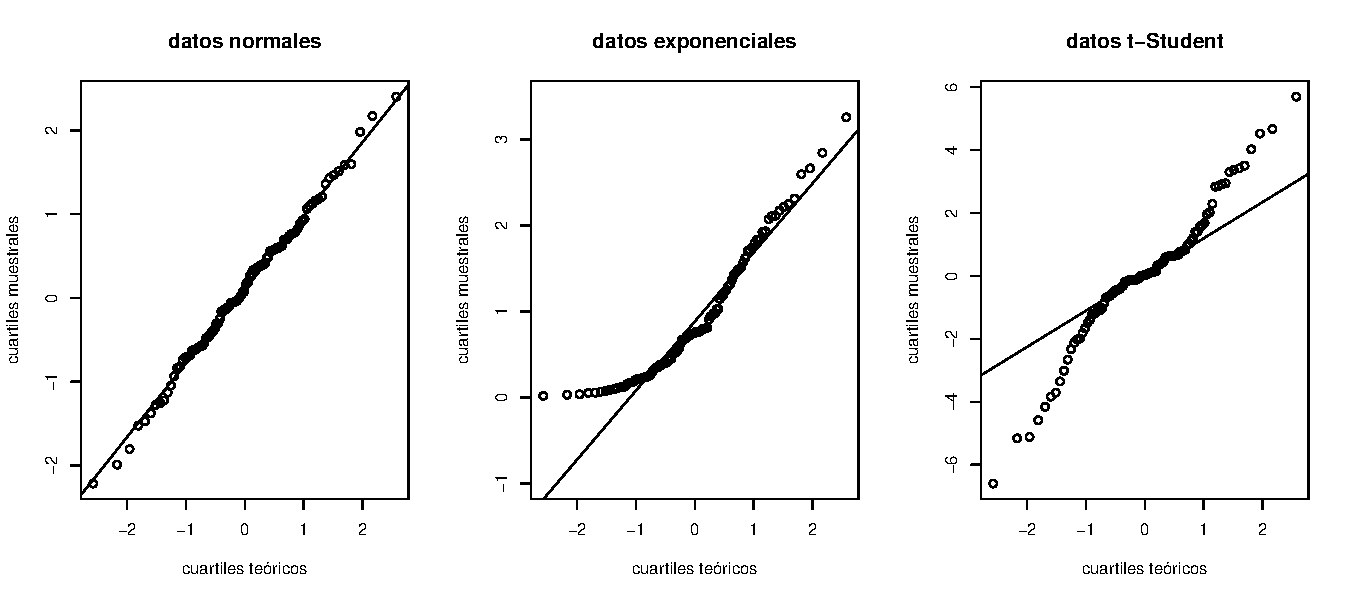
\includegraphics{MLG1_files/figure-latex/qqplots-1} 

}

\caption{Gráficos de normalidad para datos aleatorios generados a partir de una distribución normal estándar (izquierda), exponencial (centro), y t-Student con 2 grados de libertad (derecha).}\label{fig:qqplots}
\end{figure}

\rule{\textwidth}{0.4pt}

\hypertarget{bajo-peso-al-nacer---gruxe1fico-de-normalidad}{%
\paragraph*{Bajo peso al nacer - gráfico de normalidad}\label{bajo-peso-al-nacer---gruxe1fico-de-normalidad}}
\addcontentsline{toc}{paragraph}{Bajo peso al nacer - gráfico de normalidad}

El gráfico cuartil-cuartil de los residuos estudentizados se obtiene así:

\begin{Shaded}
\begin{Highlighting}[]
\NormalTok{car}\SpecialCharTok{::}\FunctionTok{qqPlot}\NormalTok{(mod.birthweight,}\AttributeTok{xlab=}\StringTok{\textquotesingle{}cuantiles teóricos\textquotesingle{}}\NormalTok{,}\AttributeTok{ylab=}\StringTok{\textquotesingle{}residuos estudentizados\textquotesingle{}}\NormalTok{,}
       \AttributeTok{distribution =} \StringTok{\textquotesingle{}norm\textquotesingle{}}\NormalTok{)}
\end{Highlighting}
\end{Shaded}

\begin{figure}

{\centering 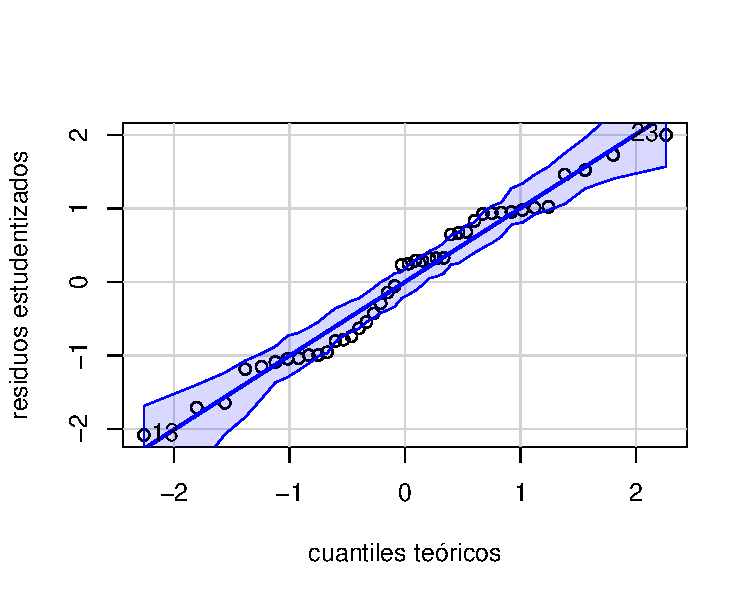
\includegraphics{MLG1_files/figure-latex/qqnormBWdata1-1} 

}

\caption{Datos de peso al nacer. Gráfico cuantil-cuantil para normalidad.}\label{fig:qqnormBWdata1}
\end{figure}

\begin{verbatim}
## [1] 13 23
\end{verbatim}

Note que la función \texttt{qqPlot} incluye intervalos del \(95\%\) de confianza para los estadísticos de orden. Para más detalle de como se calculan, ver Sección 12.1.1 de \citet{fox_applied_2016}.

La Figura \ref{fig:qqnormBWdata1} muestra que los puntos siguen de forma aproximada una línea recta. Además, la mayoría de los puntos están dentro de las bandas de confianza. Por lo tanto, se estaría cumpliendo el supuesto de normalidad.

\rule{\textwidth}{0.4pt}

\hypertarget{gruxe1fico-de-residuos-frente-a-el-tiempo}{%
\subsubsection{Gráfico de residuos frente a el tiempo}\label{gruxe1fico-de-residuos-frente-a-el-tiempo}}

Cómo se mencionó anteriormente, si las observaciones fueron tomadas de forma independiente, entonces se puede garantizar que los errores también lo sean. Para los datos del peso de los recién nacidos, tendríamos que asumir que los bebés fueron seleccionados de forma totalmente aleatoria, y así garantizar que los errores no están correlacionados. Por el contrario, los datos del consumo de helado fueron tomados a lo largo del tiempo (cada dos semanas), por lo que se puede presentar \textbf{correlación temporal}. Es decir, observaciones tomadas en tiempo cercanos se espera que estén altamente correlacionadas.

En caso de posible correlación temporal, se puede hacer un gráfico de los residuos con respecto al tiempo. Alternativamente, se puede hacer un gráfico de los residuos rezagados. Es decir, los residuos en el tiempo \(t\) (\(e_{t}\)) contra los residuos en el tiempo inmediatamente anterior \((e_{t-1})\).

La Figura \ref{fig:residuosCorr} muestra diferentes patrones de comportamiento para residuos correlacionados temporalmente. En la columna (a) vemos el comportamiento de residuos incorrelacionados. Estos fluctúan alrededor de cero sin mostrar ningún patrón claro, además el gráfico de residuos rezagados no muestra niguna tendencia. Por el contrario, en las columnas (b) y (c) vemos patrones de comportamiento de residuos correlacionados de forma positiva y negativa, respectivamente. Cuando hay correlación positiva, los valores de los residuos que están cercanos en el tiempo tienden a ser muy similares, además el gráfico de los residuos rezagados muestra una relación positiva entre \(e_{t}\) y \(e_{t-1}\). Cuando la correlación es negativa, vemos que los residuos en el tiempo cambian de signo constantemente, además el gráfico de residuos rezagados muestra una tendencia negativa.

\begin{figure}

{\centering 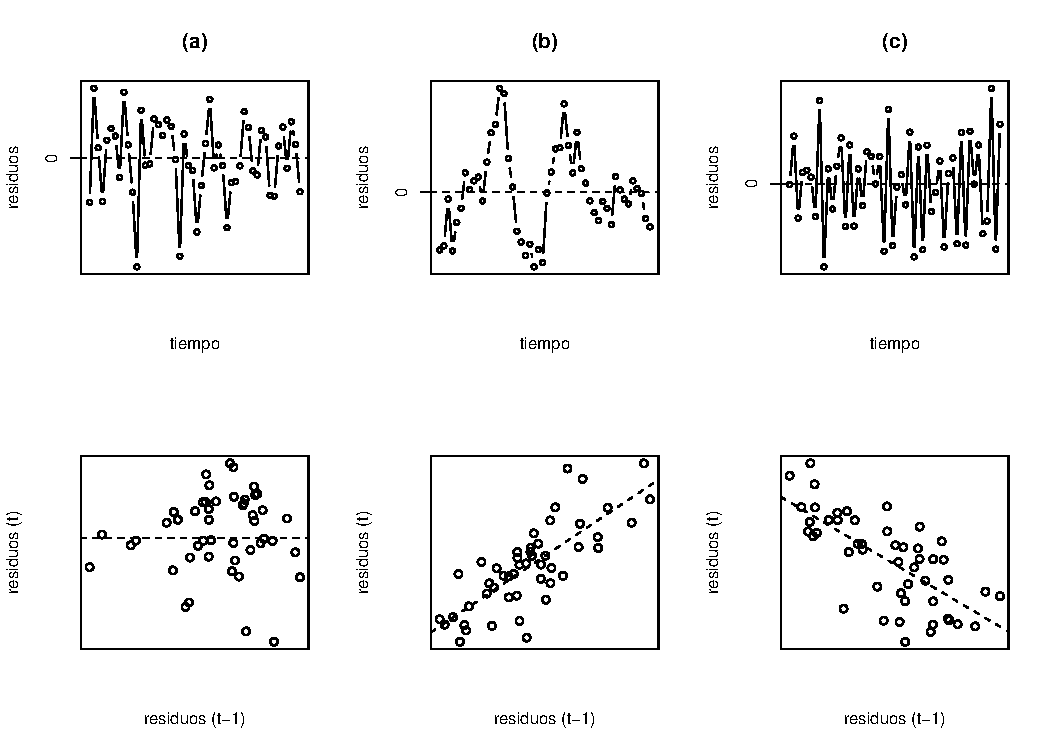
\includegraphics{MLG1_files/figure-latex/residuosCorr-1} 

}

\caption{Patrones de correlación temporal de los residuos. En la columna (a) los residuos están incorrelacionados, (b) los residuos tienen correlación positiva, y en (c) los residuos tienen correlación negativa.}\label{fig:residuosCorr}
\end{figure}
\rule{\textwidth}{0.4pt}

\hypertarget{consumo-de-helado---gruxe1fico-de-los-residuos-contra-el-tiempo}{%
\paragraph*{Consumo de helado - gráfico de los residuos contra el tiempo}\label{consumo-de-helado---gruxe1fico-de-los-residuos-contra-el-tiempo}}
\addcontentsline{toc}{paragraph}{Consumo de helado - gráfico de los residuos contra el tiempo}

Los gráficos de los residuos para el modelo ajustado a los datos de consumo de helado se observan en la Figura \ref{fig:heladosResiduos1}. Aquí vemos que la relación entre la variable respuesta y las covariables es aproximadamente lineal, no hay problemas de heterocedasticidad, y que los residuos siguen una distribución normal. Aunque se ve la presencia de un punto atípico.

\begin{Shaded}
\begin{Highlighting}[]
\NormalTok{res.stud.icecream }\OtherTok{=} \FunctionTok{studres}\NormalTok{(mod.icecream)}
\NormalTok{mod.fit.icecream }\OtherTok{=}\NormalTok{ mod.icecream}\SpecialCharTok{$}\NormalTok{fitted.values}
\FunctionTok{par}\NormalTok{(}\AttributeTok{mfrow=}\FunctionTok{c}\NormalTok{(}\DecValTok{1}\NormalTok{,}\DecValTok{2}\NormalTok{))}
\FunctionTok{plot}\NormalTok{(mod.fit.icecream,res.stud.icecream, }\AttributeTok{ylab=}\StringTok{\textquotesingle{}residuos estudentizados\textquotesingle{}}\NormalTok{,}
     \AttributeTok{xlab=}\StringTok{\textquotesingle{}valores ajustados\textquotesingle{}}\NormalTok{)}
\FunctionTok{abline}\NormalTok{(}\AttributeTok{h=}\DecValTok{0}\NormalTok{,}\AttributeTok{lty=}\DecValTok{2}\NormalTok{)}
\FunctionTok{lines}\NormalTok{(}\FunctionTok{lowess}\NormalTok{(res.stud.icecream}\SpecialCharTok{\textasciitilde{}}\NormalTok{mod.fit.icecream), }\AttributeTok{col =} \DecValTok{2}\NormalTok{)}
\NormalTok{car}\SpecialCharTok{::}\FunctionTok{qqPlot}\NormalTok{(mod.icecream,}\AttributeTok{xlab=}\StringTok{\textquotesingle{}cuantiles teóricos\textquotesingle{}}\NormalTok{,}\AttributeTok{ylab=}\StringTok{\textquotesingle{}residuos estudentizados\textquotesingle{}}\NormalTok{,}
       \AttributeTok{distribution =} \StringTok{\textquotesingle{}norm\textquotesingle{}}\NormalTok{)}
\end{Highlighting}
\end{Shaded}

\begin{figure}

{\centering 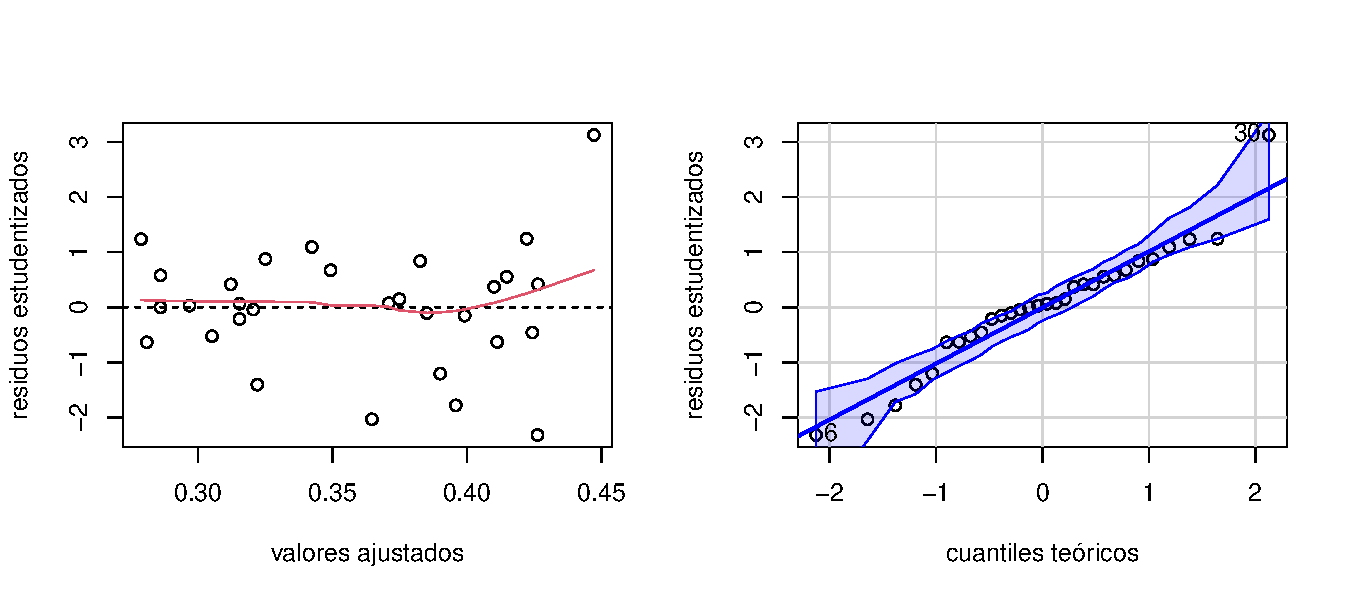
\includegraphics{MLG1_files/figure-latex/heladosResiduos1-1} 

}

\caption{Datos de consumo de helado. Gráfico de los residuos estudentizados contra los valores ajustados (izquierda) y gráfico de normalidad (derecha).}\label{fig:heladosResiduos1}
\end{figure}

\begin{verbatim}
## [1]  6 30
\end{verbatim}

Dado que las observaciones del consumo de helado tienen un orden temporal (fueron tomadas cada 4 semanas), se pueden graficar los residuos contra el tiempo y de los residuos rezagados. Estos se pueden observar en la Figura \ref{fig:heladosResiduos2}. Aquí podemos ver que hay una correlación temporal positiva. Además, se tiene que \(cor(e_{t},e_{t-1}) = 0.605\).

\begin{Shaded}
\begin{Highlighting}[]
\FunctionTok{par}\NormalTok{(}\AttributeTok{mfrow=}\FunctionTok{c}\NormalTok{(}\DecValTok{1}\NormalTok{,}\DecValTok{2}\NormalTok{))}
\FunctionTok{plot}\NormalTok{(res.stud.icecream, }\AttributeTok{ylab=}\StringTok{\textquotesingle{}residuos estudentizados\textquotesingle{}}\NormalTok{,}
     \AttributeTok{xlab=}\StringTok{\textquotesingle{}tiempo\textquotesingle{}}\NormalTok{,}\AttributeTok{type=}\StringTok{\textquotesingle{}b\textquotesingle{}}\NormalTok{)}
\FunctionTok{abline}\NormalTok{(}\AttributeTok{h=}\DecValTok{0}\NormalTok{,}\AttributeTok{lty=}\DecValTok{2}\NormalTok{)}
\FunctionTok{plot}\NormalTok{(res.stud.icecream[}\SpecialCharTok{{-}}\DecValTok{30}\NormalTok{],res.stud.icecream[}\SpecialCharTok{{-}}\DecValTok{1}\NormalTok{], }\AttributeTok{ylab=}\StringTok{\textquotesingle{}residuos estudentizados (t)\textquotesingle{}}\NormalTok{,}
     \AttributeTok{xlab=}\StringTok{\textquotesingle{}residuos estudentizados (t{-}1)\textquotesingle{}}\NormalTok{)}
\FunctionTok{abline}\NormalTok{(}\FunctionTok{lm}\NormalTok{(res.stud.icecream[}\SpecialCharTok{{-}}\DecValTok{1}\NormalTok{] }\SpecialCharTok{\textasciitilde{}}\NormalTok{ res.stud.icecream[}\SpecialCharTok{{-}}\DecValTok{30}\NormalTok{]),}\AttributeTok{lty=}\DecValTok{2}\NormalTok{)}
\end{Highlighting}
\end{Shaded}

\begin{figure}

{\centering 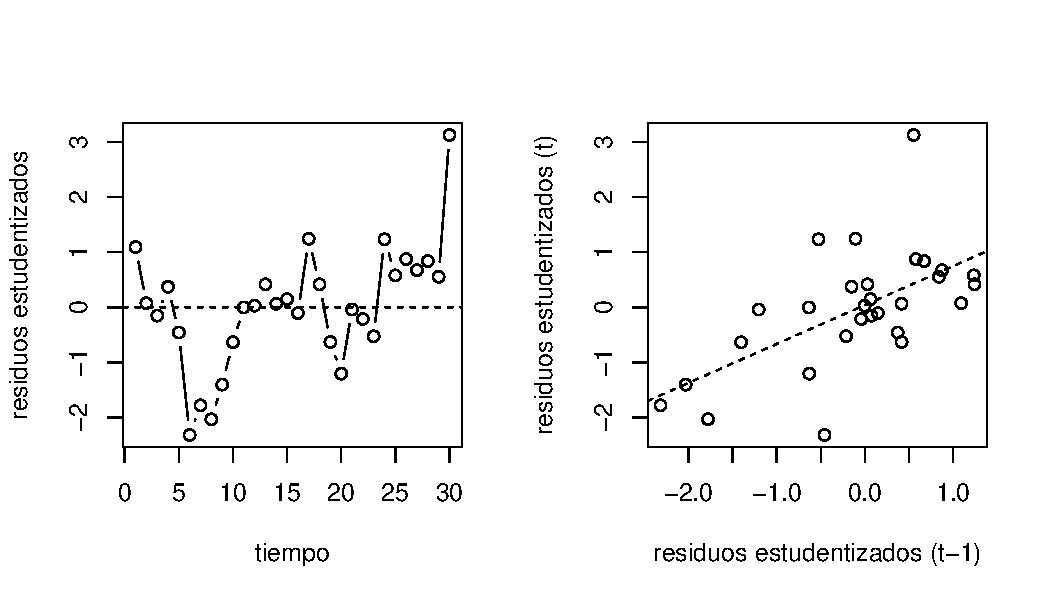
\includegraphics{MLG1_files/figure-latex/heladosResiduos2-1} 

}

\caption{Datos de consumo de helado. Gráfico de los residuos estudentizados contra el tiempo (izquierda) y gráfico de residuos rezagados (derecha).}\label{fig:heladosResiduos2}
\end{figure}
\rule{\textwidth}{0.4pt}

\hypertarget{pruebas-de-hipuxf3tesis-para-evaluar-los-supuestos}{%
\subsection{Pruebas de hipótesis para evaluar los supuestos}\label{pruebas-de-hipuxf3tesis-para-evaluar-los-supuestos}}

\hypertarget{prueba-de-falta-de-ajuste}{%
\subsubsection{Prueba de falta de ajuste}\label{prueba-de-falta-de-ajuste}}

El objetivo de la prueba de falta de ajuste es determinar si la relación entre la variable respuesta y las covariables puede asumirse cómo lineal. Hay que tener en cuenta que esta prueba es sensible a ajamientos de los supuestos de normalidad, varianza constante e independencia de los errores. Además, requiere que se tengan mútiple observaciones de \(y\) para diferentes niveles de \(\boldsymbol x\). Por ejemplo, el test puede implementarse en los datos de la longitud de los peces puesto que tenemos varios individuos con las mismas edades. En los otros casos, no es posible, por lo menos de forma exacta. El objetivo de estas observaciones replicadas es tener una estimación independiente de \(\sigma^{2}\).

En regresión lineal simple, suponga que se tienen \(n_{i}\) observaciones de la variable respuesta para el \(i\)-ésimo nivel de \(x_{i}\), para \(i=1,\ldots,m\), y denotemos \(y_{ij}\) como la \(j\)-ésima observación de la respuesta en \(x_{i}\), para \(j=1,\ldots,n_{i}\). Por lo tanto, tenemos \(n=\sum_{i=1}^{m}n_{i}\) observaciones en total. Esto permite que se puede descomponer la suma de cuadrados de los residuos en dos:
\[
SS_{res} = SS_{PE} + SS_{LOF},
\]
donde \(SS_{PE}\) y \(SS_{LOF}\) son la suma de cuadrados del error puro y falta de ajuste, respectivamente.

Para esto, primero observemos que los residuos se pueden descomponer así:
\begin{equation}
y_{ij} - \widehat{y}_{i} = (y_{ij} - \bar{y}_{i}) + (\bar{y}_{i} - \widehat{y}_{i}),
\label{eq:ssresd}
\end{equation}
donde \(\bar{y}_{i}\) es el promedio de las \(n_{i}\) observaciones en \(x_{i}\). Ahora, elevando al cuadrado ambos lados de \eqref{eq:ssresd}, y sumando para todo \(i\) y \(j\), tenemos:
\begin{equation}
\begin{split}
\sum_{i=1}^{m} \sum_{j=1}^{n_{i}} (y_{ij} - \widehat{y}_{i})^{2} &= \sum_{i=1}^{m}\sum_{j=1}^{n_{i}}(y_{ij}-\bar{y}_{i})^{2} + \sum_{i=1}^{m}n_{i}(\bar{y}_{i}-\widehat{y}_{i})^{2}, \\
SS_{res} &= SS_{PE} + SS_{LOF}.
\end{split}
\nonumber
\end{equation}

Note que la suma de cuadrados de la falta de ajuste es una suma ponderada de las diferencias entre el promedio de las observaciones en cada nivel de \(x\) y el correspondiente valor ajustado. Por lo tanto, si la relación entre las variables es aproximadamente lineal, entonces se espera que \(SS_{LOF}\) sea cercana a cero.

Los grados de libertad de \(SS_{PE}\) y \(SS_{LOF}\) son \(\sum_{i=1}^{m}(n_{i}-1) = n-m\) y \(m-2\), respectivamente. De aquí se define el cuadrado medio del error puro y el cuadrado medio de la falta de ajuste:

\[
MS_{PE} = \frac{SS_{PE}}{n-m} \mbox{ y } MS_{LOF} = \frac{SS_{LOF}}{m-2},
\]

respectivamente. Si se cumple el supuesto de homocedasticidad, el valor esperado de \(MS_{PE}\) es:
\[
E(MS_{PE}) = \frac{1}{n-m}E\left[ \sum_{j=1}^{n_{i}}(y_{ij} - \widehat{y}_{i})^{2} \right] = \frac{1}{n-m}\sum_{j=1}^{n_{i}} E\left[ (y_{ij}-\widehat{y}_{i})^{2} \right] = \frac{\sigma^{2}}{n-m}\sum_{j=1}^{n_{i}}(n_{i}-1) = \sigma^{2}.
\]
Es decir que el cuadrado medio del error puro es una estimación de \(\sigma^{2}\) independiente del ajuste del modelo.

Además, el valor esperado del cuadrado medio de la falta de ajuste es:
\[
E(MS_{LOF}) = \sigma^{2} + \frac{\sum_{i=1}^{m}n_{i}\left[ E(y_{i}|x_{i}) - \beta_{0}-\beta_{1}x_{i} \right]^{2}}{m-2}.
\]
Por lo tanto, si la función de la media es lineal, entonces \(E(y_{i}|x_{i}) = \beta_{0}+\beta_{1}x_{i}\), y \(E(MS_{LOF}) = \sigma^{2}\). Si la función media no es lineal, entonces \(E(MS_{LOF}) > \sigma^{2}\)

La prueba de falta de ajuste plantea las siguiente hipótesis:
\[
H_{0}: \mbox{el lineal modelo proporciona buen ajuste} \qquad H_{1}: \mbox{el modelo lineal no proporciona buen ajuste},
\]
El estadístico de prueba es:
\[
F_{0}=\frac{SS_{LOF}/(m-2)}{SS_{PE}/(n-m)} = \frac{MS_{LOF}}{MS_{PE}}.
\]
Si \(H_{0}\) es cierta, \(F_{0}\) sigue una distribución \(F_{m-2,n-m}\). Por lo tanto, se rechaza \(H_{0}\) (es decir, la función de regresión no es lineal) si \(F_{0} > F_{1-\alpha,m-2,n-m}\).

Como se mencionó antes, la prueba exige que se tenga múltiples observaciones para cada nivel de \(x\). Lo cuál es un gran desventaja. En caso que esto no ocurra, se puede hacer agrupaciones de los valores de las covariables (vecinos más cercanos), y considerarlas como repeticiones; de esta manera la prueba es aproximada.

\rule{\textwidth}{0.4pt}

\hypertarget{base-de-datos-de-la-longitud-de-los-peces---prueba-de-falta-de-ajuste}{%
\paragraph{Base de datos de la longitud de los peces - prueba de falta de ajuste}\label{base-de-datos-de-la-longitud-de-los-peces---prueba-de-falta-de-ajuste}}

La Figura \ref{fig:pecesResiduos1} muestra los gráficos de los residuos para el modelo ajustado a los datos de la longitud de los peces.

\begin{Shaded}
\begin{Highlighting}[]
\NormalTok{res.stud.bass }\OtherTok{=} \FunctionTok{studres}\NormalTok{(mod.bass)}
\NormalTok{mod.fit.bass }\OtherTok{=}\NormalTok{ mod.bass}\SpecialCharTok{$}\NormalTok{fitted.values}
\FunctionTok{plot}\NormalTok{(mod.fit.bass,res.stud.bass, }\AttributeTok{ylab=}\StringTok{\textquotesingle{}residuos estudentizados\textquotesingle{}}\NormalTok{,}
     \AttributeTok{xlab=}\StringTok{\textquotesingle{}valores ajustados\textquotesingle{}}\NormalTok{)}
\FunctionTok{abline}\NormalTok{(}\AttributeTok{h=}\DecValTok{0}\NormalTok{,}\AttributeTok{lty=}\DecValTok{2}\NormalTok{)}
\FunctionTok{lines}\NormalTok{(}\FunctionTok{lowess}\NormalTok{(res.stud.bass}\SpecialCharTok{\textasciitilde{}}\NormalTok{mod.fit.bass), }\AttributeTok{col =} \DecValTok{2}\NormalTok{)}
\end{Highlighting}
\end{Shaded}

\begin{figure}

{\centering 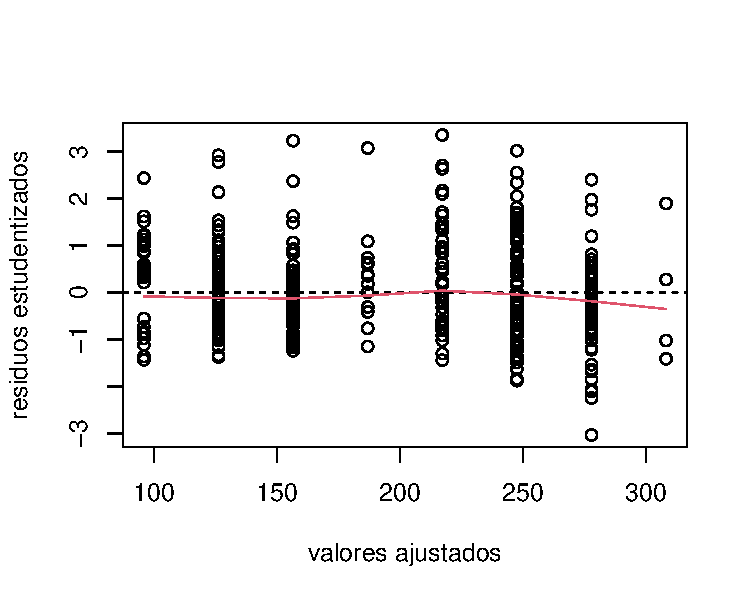
\includegraphics{MLG1_files/figure-latex/pecesResiduos1-1} 

}

\caption{Datos de la longitud de los peces. Gráfico de los residuos estudentizados contra los valores ajustados.}\label{fig:pecesResiduos1}
\end{figure}

La prueba de falta se ajuste se puede hacer usando la función \texttt{anovaPE} de la librería \texttt{EnvStats}:

\begin{Shaded}
\begin{Highlighting}[]
\FunctionTok{library}\NormalTok{(EnvStats)}
\FunctionTok{anovaPE}\NormalTok{(mod.bass)}
\end{Highlighting}
\end{Shaded}

\begin{verbatim}
##                 Df  Sum Sq Mean Sq   F value Pr(>F)    
## Age              1 1595359 1595359 1973.0736 <2e-16 ***
## Lack of Fit      6   10104    1684    2.0827 0.0541 .  
## Pure Error     431  348492     809                     
## ---
## Signif. codes:  0 '***' 0.001 '**' 0.01 '*' 0.05 '.' 0.1 ' ' 1
\end{verbatim}

A partir del valor-\(p\) podemos concluir que no se rechaza \(H_{0}\), por lo tanto no hay suficiente evidencia para dudar del ajuste lineal propuesto.

\rule{\textwidth}{0.4pt}

\hypertarget{prueba-de-heterocedasticidad}{%
\subsubsection{Prueba de heterocedasticidad}\label{prueba-de-heterocedasticidad}}

Algunas pruebas de heterocedasticidad asumen que la varianza de los errores se compone de una parte constante y otra que varía según unas variables \((\boldsymbol z)\):
\[
\sigma^{2}_{i} = f(\sigma^{2},\boldsymbol z_{i}),
\]
donde \(\sigma^{2}\) es la parte fija de la varianza, \(\boldsymbol z_{i}\) el conjunto de variables cuyos valores se asocian con los cambios en la varianza de los errores. Por lo general se asume que la función de varianza depende de algunas de las covariables del modelo, es decir que \(\boldsymbol z_{i}=\boldsymbol x_{i}\).

La \textbf{prueba de Breusch-Pagan} asume que la varianza es una función aditiva de las covariables:
\[
\sigma^{2}_{i} = E(\varepsilon_{i}^{2}) = \gamma_{0} + \gamma_{1}x_{i1}+ \gamma_{1}x_{i2} + \ldots  + \gamma_{p-1}x_{i,p-1}.
\]

Por lo tanto, se pueden plantear las siguientes hipótesis:
\begin{equation}
\begin{split}
H_{0}:& \gamma_{1} = \gamma_{2} = \ldots = \gamma_{p-1} = 0 \qquad \mbox{ (homocedasticidad)}, \\
H_{1}:& \gamma_{j}\neq 0 \mbox{ para algún }j=1,\ldots,p-1 \mbox{ (heterocedasticidad)}.
\end{split}
\nonumber
\end{equation}
Dado que los errores no son observables, el estadístico de prueba se construye a partir de los residuos del modelo estimado. Primero, se ajusta el siguiente modelo de regresión:
\[
e_{i}^{2} = \gamma_{0} + \gamma_{1}x_{i1}+ \gamma_{1}x_{i2} + \ldots  + \gamma_{p-1}x_{i,p-1} + \upsilon_{i},
\]
donde se asume que \(\upsilon_{i}\sim N(0,\sigma^{2}_{\upsilon})\), y se obtiene el coeficiente de determinación \(R^{2}_{e}\).

si \(H_{0}\) es cierta, se tiene que \(W = n R^{2}_{e} \sim \chi^{2}_{p-1}\). Entonces, si \(W > \chi^{2}_{1-\alpha,p-1}\) se rechaza \(H_{0}\). Por lo tanto, hay heterocedasticidad.

El test de Breusch-Pagan sólo detecta formas lineales de heterocedasticidad. La \textbf{prueba de White} propone que la relación entre la varianza y las covariables es cuadrática:
\begin{equation}
\begin{split}
\sigma^{2}_{i} &= \left(\gamma_{0}^{*} + \sum_{j=1}^{p-1}\gamma_{j}^{*}x_{ij}\right)^{2} \\
&= \gamma_{0} + \sum_{j=1}^{p-1}\gamma_{j}x_{ij} + \sum_{j=1}^{p-1}\gamma_{jj}x_{ij}^{2} + \sum_{j=1}^{p-1}\sum_{k \neq j}\gamma_{jk}x_{ij}x_{ik}.
\end{split}
\nonumber
\end{equation}
Dado que el número de parámetros del modelo se incrementa rápidamente a medida que tengamos más covariables, se pueden omitir las interacciones entre las covariables.

Por ejemplo si se tiene un modelo con tres covariables, se plantea la siguiente función para la varianza:
\[
\sigma^{2}_{i} = \gamma_{0} + \gamma_{1}x_{i1} + \gamma_{1}x_{i2}  + \gamma_{1}x_{i3} + \gamma_{4}x_{i1}^{2}+\gamma_{5}x_{i2}^{2} + \gamma_{6}x_{i3}^{2} + \gamma_{7}x_{i1}x_{i2} + \gamma_{8}x_{i1}x_{i3} + \gamma_{9}x_{i2}x_{i3}
\]
y las hipótesis son:
\begin{equation}
\begin{split}
H_{0}:& \gamma_{1} = \gamma_{2} = \ldots = \gamma_{9} = 0 \qquad \mbox{ (homocedasticidad)}, \\
H_{1}:& \gamma_{j}\neq 0 \mbox{ para algún }j=1,\ldots,9 \mbox{ (heterocedasticidad)}.    
\end{split}
\nonumber
\end{equation}
Para calcular el estadístico de prueba, primero ajustamos el siguiente modelo auxiliar:
\[
e_{i}^{2} = \gamma_{0} + \gamma_{1}x_{i1} + \gamma_{1}x_{i2}  + \gamma_{1}x_{i3} + \gamma_{4}x_{i1}^{2}+\gamma_{5}x_{i2}^{2} + \gamma_{6}x_{i3}^{2} + \gamma_{7}x_{i1}x_{i2} + \gamma_{8}x_{i1}x_{i3} + \gamma_{9}x_{i2}x_{i3} + \upsilon_{i},
\]
y el coeficiente de determinación asociado \(R_{e}^{2}\). El estadístico de prueba es \(W=nR_{e}^{2}\), y rechazamos \(H_{0}\) si \(W > \chi^{2}_{1-\alpha,8}\).

\rule{\textwidth}{0.4pt}

\hypertarget{bajo-peso-al-nacer---prueba-de-heterocedasticidad}{%
\paragraph*{Bajo peso al nacer - prueba de heterocedasticidad}\label{bajo-peso-al-nacer---prueba-de-heterocedasticidad}}
\addcontentsline{toc}{paragraph}{Bajo peso al nacer - prueba de heterocedasticidad}

En la prueba de White se asume que:
\begin{equation}
\begin{split}
\sigma^{2}_{i} =& \gamma_{0} + \gamma_{1}\mbox{age}_{i} + \gamma_{2}\mbox{motherage}_{i}  + \gamma_{3}\mbox{mnocig}_{i} + \gamma_{4}\mbox{mppwt}_{i}+ \\
& \gamma_{5}\mbox{age}_{i}^{2} + \gamma_{6}\mbox{motherage}_{i}^{2}  + \gamma_{7}\mbox{mnocig}_{i}^{2} + \gamma_{8}\mbox{mppwt}_{i}^{2}.
\end{split}
\nonumber
\end{equation}
Dado que se tienen varias covariables, se omitieron las interacciones entre las covariables. Se plantean las siguientes hipótesis:
\begin{equation}
\begin{split}
H_{0}:& \gamma_{1} = \gamma_{2} = \ldots = \gamma_{8} = 0 \qquad \mbox{ (homocedasticidad)}, \\
H_{1}:& \gamma_{j}\neq 0 \mbox{ para algún }j=1,\ldots,8 \mbox{ (heterocedasticidad)}.
\end{split}
\nonumber
\end{equation}
El ajuste del modelo auxiliar es:

\begin{Shaded}
\begin{Highlighting}[]
\NormalTok{res.stud.birthweight}\OtherTok{=}\NormalTok{mod.birthweight}\SpecialCharTok{$}\NormalTok{residuals}
\NormalTok{mod.res.birthweight }\OtherTok{=} \FunctionTok{lm}\NormalTok{(res.stud.birthweight}\SpecialCharTok{\^{}}\DecValTok{2} \SpecialCharTok{\textasciitilde{}}\NormalTok{ age }\SpecialCharTok{+}\NormalTok{ motherage }\SpecialCharTok{+}\NormalTok{ mnocig }\SpecialCharTok{+}\NormalTok{ mppwt }\SpecialCharTok{+}
                           \FunctionTok{I}\NormalTok{(age}\SpecialCharTok{\^{}}\DecValTok{2}\NormalTok{) }\SpecialCharTok{+} \FunctionTok{I}\NormalTok{(motherage}\SpecialCharTok{\^{}}\DecValTok{2}\NormalTok{) }\SpecialCharTok{+} \FunctionTok{I}\NormalTok{(mnocig}\SpecialCharTok{\^{}}\DecValTok{2}\NormalTok{) }\SpecialCharTok{+} \FunctionTok{I}\NormalTok{(mppwt}\SpecialCharTok{\^{}}\DecValTok{2}\NormalTok{), }
                         \AttributeTok{data=}\NormalTok{birthweight)}
\FunctionTok{summary}\NormalTok{(mod.res.birthweight)}
\end{Highlighting}
\end{Shaded}

\begin{verbatim}
## 
## Call:
## lm(formula = res.stud.birthweight^2 ~ age + motherage + mnocig + 
##     mppwt + I(age^2) + I(motherage^2) + I(mnocig^2) + I(mppwt^2), 
##     data = birthweight)
## 
## Residuals:
##      Min       1Q   Median       3Q      Max 
## -0.20691 -0.08384 -0.01338  0.02286  0.41575 
## 
## Coefficients:
##                  Estimate Std. Error t value Pr(>|t|)  
## (Intercept)    -6.1348535  3.4447222  -1.781   0.0841 .
## age             0.2877513  0.1701394   1.691   0.1002  
## motherage      -0.0406689  0.0359059  -1.133   0.2655  
## mnocig          0.0024339  0.0051823   0.470   0.6417  
## mppwt           0.0433585  0.0435969   0.995   0.3272  
## I(age^2)       -0.0037481  0.0021924  -1.710   0.0967 .
## I(motherage^2)  0.0007444  0.0006445   1.155   0.2563  
## I(mnocig^2)    -0.0001672  0.0001335  -1.253   0.2192  
## I(mppwt^2)     -0.0003450  0.0003688  -0.935   0.3564  
## ---
## Signif. codes:  0 '***' 0.001 '**' 0.01 '*' 0.05 '.' 0.1 ' ' 1
## 
## Residual standard error: 0.1457 on 33 degrees of freedom
## Multiple R-squared:  0.2397, Adjusted R-squared:  0.05544 
## F-statistic: 1.301 on 8 and 33 DF,  p-value: 0.2772
\end{verbatim}

Note que el estadístico \(F_{0}\) es pequeño y que las pruebas individuales sobre los coeficientes no son significativas. Esto es un indicio que \(H_{0}\) es cierta. El coeficiente de determinación es \(R_{e}^{2} = 0.24\). Entonces, \(W= 10.069\), con un valor-\(p\) asociado de \(0.2602\). Por lo tanto, no tenemos evidencia suficiente para determinar que hay heterocedasticidad.

La prueba se puede implementar directamente usando la función \texttt{bptest} de la librería \texttt{lmtest} llegando a los mismos resultados:

\begin{Shaded}
\begin{Highlighting}[]
\FunctionTok{bptest}\NormalTok{(mod.birthweight, }\SpecialCharTok{\textasciitilde{}}\NormalTok{ age }\SpecialCharTok{+}\NormalTok{ motherage }\SpecialCharTok{+}\NormalTok{ mnocig }\SpecialCharTok{+}\NormalTok{ mppwt }\SpecialCharTok{+}
                           \FunctionTok{I}\NormalTok{(age}\SpecialCharTok{\^{}}\DecValTok{2}\NormalTok{) }\SpecialCharTok{+} \FunctionTok{I}\NormalTok{(motherage}\SpecialCharTok{\^{}}\DecValTok{2}\NormalTok{) }\SpecialCharTok{+} \FunctionTok{I}\NormalTok{(mnocig}\SpecialCharTok{\^{}}\DecValTok{2}\NormalTok{) }\SpecialCharTok{+} \FunctionTok{I}\NormalTok{(mppwt}\SpecialCharTok{\^{}}\DecValTok{2}\NormalTok{), }
                         \AttributeTok{data=}\NormalTok{birthweight)}
\end{Highlighting}
\end{Shaded}

\begin{verbatim}
## 
##  studentized Breusch-Pagan test
## 
## data:  mod.birthweight
## BP = 10.069, df = 8, p-value = 0.2602
\end{verbatim}

\rule{\textwidth}{0.4pt}

Otras pruebas de heterocedasticidad que se pueden utilizar son:

\begin{itemize}
\tightlist
\item
  Prueba de Goldfeld--Quandt.
\item
  Prueba de Barlett.
\item
  Prueba de Cochran.
\item
  Prueba de Hartley.
\end{itemize}

Las últimas tres pruebas requieren que se tengan múltiples observaciones para cada nivel de \(\boldsymbol x\). En caso que no se tengan repeticiones, es posible agruparlas por los vecinos más cercanos e implementar la prueba de forma aproximada.

\hypertarget{prueba-de-normalidad}{%
\subsubsection{Prueba de normalidad}\label{prueba-de-normalidad}}

Para probar normalidad podemos utilizar la prueba de Shapiro-Wilks.

Suponga que se tiene una muestra aleatoria \(x_{1},\ldots,x_{n}\) que se asumen sigue una distribución normal. Por lo cuál, se plantean las siguientes hipótesis:
\[
H_{0}: \mbox{la distribución de }X \mbox{ es normal} \qquad H_{0}: \mbox{la distribución de }X \mbox{ no es normal}
\]
El estadístico de prueba propuestos por Shapiro y Wilks es:
\[
W = \frac{ \sum_{i=1}^{[n/2]}a_{in}\left(x_{[n-i+1]}-x_{[i]}\right)  }{\sum_{i=1}^{n}(x_{i}-\bar{x})^{2}},
\]
donde \((x_{[1]},x_{[2]},\ldots,x_{[n]})\) son los estadísticos de orden y los valores \(a_{in}\), así como los valores críticos, están dados en tablas tabuladas por los autores.

\rule{\textwidth}{0.4pt}

\hypertarget{bajo-peso-al-nacer---prueba-de-normalidad}{%
\paragraph*{Bajo peso al nacer - prueba de normalidad}\label{bajo-peso-al-nacer---prueba-de-normalidad}}
\addcontentsline{toc}{paragraph}{Bajo peso al nacer - prueba de normalidad}

La prueba de Shapiro-Wilks para ajuste de los datos de peso al nacer es:
\texttt{lmtest}:

\begin{Shaded}
\begin{Highlighting}[]
\FunctionTok{shapiro.test}\NormalTok{(res.stud.birthweight)}
\end{Highlighting}
\end{Shaded}

\begin{verbatim}
## 
##  Shapiro-Wilk normality test
## 
## data:  res.stud.birthweight
## W = 0.96593, p-value = 0.2395
\end{verbatim}

A partir de este resultado, no tenemos evidencia suficiente para rechazar que los errores se distribuyen normal. En esta función de R, el valor-\(p\) es calculado usando una aproximación.

\rule{\textwidth}{0.4pt}

Otras pruebas de normalidad que se pueden utilizar son:

\begin{itemize}
\tightlist
\item
  Modificaciones de la prueba Shapiro-Wilks, como son: D'agostino o Shapiro-Francia.
\item
  Pruebas de bondad de ajuste generales, como son: Kolmogorov-Smirnov, Cramer-Von Mises, Anderson-Darling.
\end{itemize}

\hypertarget{prueba-de-correlaciuxf3n-temporal-de-los-errores}{%
\subsubsection{Prueba de correlación temporal de los errores}\label{prueba-de-correlaciuxf3n-temporal-de-los-errores}}

Cuando la correlación es debido a que las observaciones fueron tomadas en el tiempo, se puede asumir que hay \textbf{autocorrelación}. Aquí se asume que los errores que están separados \(t\) unidades de tiempo siempre tienen la misma correlación lineal. Además que la correlación disminuye a medida que las observaciones se separan en el tiempo.

El modelo de regresión, con errores autoregresivos de orden uno, es el siguiente:
\[
y_{t} = \boldsymbol x_{t}'\boldsymbol \beta+ \varepsilon_{t}, \mbox{ con }\varepsilon_{t}= \phi\varepsilon_{t-1} + a_{t},
\]
donde \(y_{t}\) y \(\boldsymbol x_{t}\) son la variable respuesta observada y el conjunto de covariables observadas en el tiempo \(t\), respectivamente, y \(\phi\) es el parámetro de autocorrelación \((|\phi| < 1)\). Además, se asume que \(a_{t} \sim N(0,\sigma^{2}_{a})\) y \(cov(a_{j},a_{k})=0\), para todo \(j \neq k\). A partir de estos resultados, se tiene que:
\[
E(\varepsilon_{t}) = 0, V(\varepsilon_{t}) = \sigma^{2}_{a}\left( \frac{1}{1-\phi^2}\right), \mbox{ y } cov(\varepsilon_{t},\varepsilon_{t \pm k})= \phi^{k}\sigma^{2}_{a}\left( \frac{1}{1-\phi^2} \right).
\]
Por lo tanto, la correlación entre dos errores separados en \(k\) periodos de tiempo es \(cor(\varepsilon_{t},\varepsilon_{t\pm k}) = \phi^{k}\). Si \(\phi > 0\), los errores están correlacionados positivamente, pero la magnitud de la correlación disminuye a medida que los errores se separan más. Por otro lado, si \(\phi =0\) los errores están incorrelacionados.

La prueba de Durbin-Watson plantea las siguientes hipótesis:
\[
H_{0}: \phi = 0 \mbox{ (independencia)} \qquad H_{1}:\phi \neq 0  \mbox{ (autocorrelación)}
\]
El estadístico de prueba es:
\[
d = \frac{\sum_{t=2}^{T}\left( e_{t} - e_{t-1}\right)^{2}}{\sum_{t=1}^{T}e_{t}^{2}}.
\]
La distribución de probabilidad de \(d\), bajo \(H_{0}\), depende de la estructura de \(\boldsymbol X\) y es difícil de determinar. Por lo tanto, los valores críticos están tabulados para diferentes valores de significancia, tamaño de muestra y número de parámetros. Otra alternativa, usada por los paquetes estadísticos, es calcular la significancia a través de métodos de remuestreo y aproximaciones del estadístico de prueba a la distribución normal.

\rule{\textwidth}{0.4pt}

\hypertarget{ventas-de-helado---prueba-de-correlaciuxf3n-temporal}{%
\paragraph*{Ventas de helado - prueba de correlación temporal}\label{ventas-de-helado---prueba-de-correlaciuxf3n-temporal}}
\addcontentsline{toc}{paragraph}{Ventas de helado - prueba de correlación temporal}

La prueba de Durbin-Watson para ajuste de los datos de ventas de helado se puede hacer a través de la función \texttt{durbinWatsonTest} de la librería \texttt{car}:

\begin{Shaded}
\begin{Highlighting}[]
\FunctionTok{durbinWatsonTest}\NormalTok{(mod.icecream,}\AttributeTok{method=}\StringTok{\textquotesingle{}resample\textquotesingle{}}\NormalTok{,}\AttributeTok{reps=}\DecValTok{1000}\NormalTok{)}
\end{Highlighting}
\end{Shaded}

\begin{verbatim}
##  lag Autocorrelation D-W Statistic p-value
##    1       0.5412411      0.655856       0
##  Alternative hypothesis: rho != 0
\end{verbatim}

Estos resultados muestran que hay correlación serial en los datos. Note que con esta función, el valor-\(p\) es calculado a partir de técnicas de remuestreo usando 1000 repeticiones.

\rule{\textwidth}{0.4pt}

\hypertarget{comentarios-finales}{%
\subsection{Comentarios finales}\label{comentarios-finales}}

Algunas consideraciones, muchas de ellas tomadas de \citet{behar_validacion_2002}:

\begin{itemize}
\tightlist
\item
  La efectividad de las pruebas formales depende del tamaño de la muestra. Si \(n\) es pequeño, la potencia es baja. Por lo tanto, es difícil detectar alejamientos de la hipótesis nula. Si por el contrario, la muestra es grande, la potencia es alta. Entonces, se rechaza la hipótesis nula ante cualquier alejamiento ligero.
\item
  El incumplimiento de un supuesto puede reflejarse como el incumplimiento de otros. Por ejemplo, la falta de ajuste del modelo puede reflejarse como heterogeneidad de los errores y/o como correlación de los mismos.
\item
  Hay que tener en cuenta que algunas pruebas de hipótesis suponen cierto alejamiento particular del supuesto que se quiere probar. Por ejemplo, el test de White asume que la varianza es una función cuadrática de las covariables. Por lo tanto si rechazamos esta prueba, no necesariamente podemos asegurar con total certeza que no hay heterocedasticidad. Es posible que la función de varianza tome otra forma.
\item
  Adicionalmente, varias pruebas son muy sensibles al alejamiento de la suposición de normalidad. Es decir que, si los errores no son normalmente distribuidos, el nivel real de significancia puede ser muy diferente del especificado. Sin embargo, el rechazo de la hipótesis nula podría sugerir que al menos uno de los dos supuestos no se cumple.
\item
  A la hora de validar el supuesto de normalidad de los errores se está interesado en saber si el alejamiento de ese modelo normal, es aceptable desde el punto de vista de la conservación de las propiedades y ventajas que se heredan de la normalidad. Las estimaciones de \(\widehat{\boldsymbol \beta}\) son generalmente robustas a desviaciones de la normalidad (Teorema del límite central).
\end{itemize}

\hypertarget{transformaciones-y-muxednimos-cuadrados-ordinarios}{%
\section{Transformaciones y mínimos cuadrados ordinarios}\label{transformaciones-y-muxednimos-cuadrados-ordinarios}}

\rule{\textwidth}{0.4pt}

\hypertarget{ejemplo-1.-datos-de-la-onu}{%
\subsection*{Ejemplo 1. Datos de la ONU}\label{ejemplo-1.-datos-de-la-onu}}
\addcontentsline{toc}{subsection}{Ejemplo 1. Datos de la ONU}

La base de datos \texttt{UN11} de la librería \texttt{alr4} contiene las siguientes estadísticas de varios miembros de las naciones unidas (y otras regiones independientes) durante los años 2009-2011:

\begin{itemize}
\tightlist
\item
  \textbf{fertility}: Número esperado de nacidos vivos por mujer.
\item
  \textbf{ppgdp}: producto nacional bruto per cápita (PNB, en dólares).
\item
  \textbf{Purban}: el porcentaje de la población que vive en un área urbana.
\item
  \textbf{lifeExpF}: esperanza de vida femenina (años).
\end{itemize}

El objetivo del estudio es ver la relación entre la fertilidad con las
otras variables. Por ahora, empecemos con un modelo de la fertilidad en función del producto nacional bruto y el porcentaje de población urbana.

La Figura \ref{fig:UNdataFig} muestra la relación entre las variables. Aquí vemos que ambas covariables tienen una relación negativa con la fertilidad. Note, además, que la relación con el producto nacional bruto no es lineal. Esto último podría traer problemas a la hora de ajustar un modelo lineal.

\begin{Shaded}
\begin{Highlighting}[]
\FunctionTok{library}\NormalTok{(alr4)}
\FunctionTok{data}\NormalTok{(}\StringTok{"UN11"}\NormalTok{)}
\FunctionTok{pairs}\NormalTok{(UN11[,}\SpecialCharTok{{-}}\FunctionTok{c}\NormalTok{(}\DecValTok{1}\SpecialCharTok{:}\DecValTok{2}\NormalTok{,}\DecValTok{5}\NormalTok{)])}
\end{Highlighting}
\end{Shaded}

\begin{figure}

{\centering 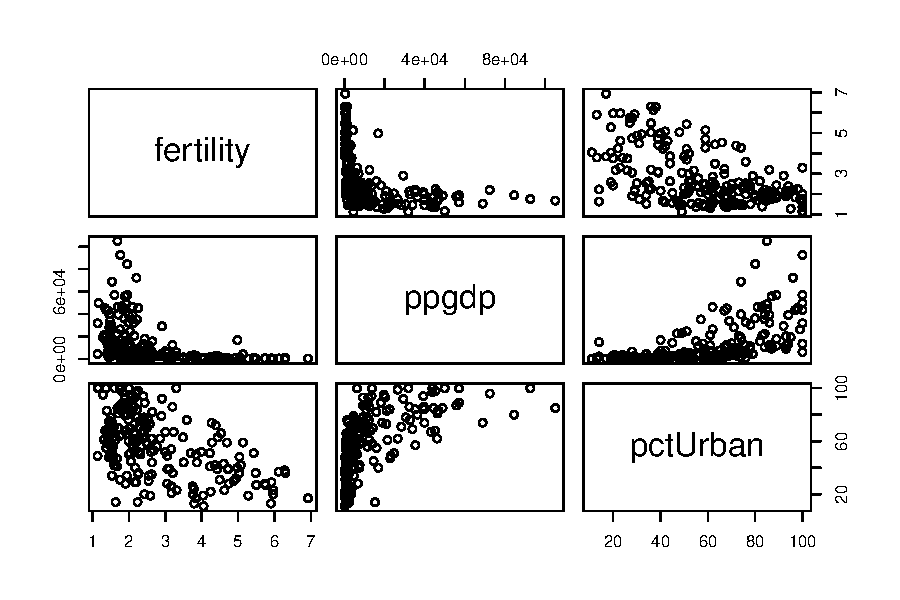
\includegraphics{MLG1_files/figure-latex/UNdataFig-1} 

}

\caption{Datos de la ONU. Relación entre las variables.}\label{fig:UNdataFig}
\end{figure}

Por ahora consideremos solamente el PNB y el \% de población en área urbana como covariables. Por lo tanto, el modelo propuesto es el siguiente:
\[
\mbox{fertility}_{i} = \beta_{0} + \beta_{1}\mbox{ppgdp}_{i} + \beta_{2}\mbox{pctUrban}_{i} + \varepsilon_{i},
\]
donde \(\varepsilon_{i}\sim N(0,\sigma^{2})\) y \(cov(\varepsilon_{j},\varepsilon_{k})=0\).

Luego de ajustar el modelo se procede a hacer un análisis de residuos. El gráfico de los residuos estudentizados (Figura \ref{fig:Un11res} muestra que el ajuste presenta problemas de no linealidad y heterocedasticidad. En la Figura \ref{fig:Un11resPartial} de los residuos parciales podemos observar que estos problemas se deben a la covariable PNB.

\begin{Shaded}
\begin{Highlighting}[]
\NormalTok{mod.UN11 }\OtherTok{=} \FunctionTok{lm}\NormalTok{(fertility}\SpecialCharTok{\textasciitilde{}}\NormalTok{ppgdp}\SpecialCharTok{+}\NormalTok{pctUrban,}\AttributeTok{data=}\NormalTok{UN11)}
\FunctionTok{library}\NormalTok{(MASS)}
\NormalTok{res.UN11 }\OtherTok{=} \FunctionTok{studres}\NormalTok{(mod.UN11)}
\FunctionTok{plot}\NormalTok{(mod.UN11}\SpecialCharTok{$}\NormalTok{fitted.values,res.UN11,}
     \AttributeTok{xlab=}\StringTok{\textquotesingle{}valores ajustados\textquotesingle{}}\NormalTok{,}\AttributeTok{ylab=}\StringTok{\textquotesingle{}residuos estudentizados\textquotesingle{}}\NormalTok{)}
\FunctionTok{lines}\NormalTok{(}\FunctionTok{lowess}\NormalTok{(res.UN11}\SpecialCharTok{\textasciitilde{}}\NormalTok{mod.UN11}\SpecialCharTok{$}\NormalTok{fitted.values),}\AttributeTok{col=}\DecValTok{2}\NormalTok{)}
\FunctionTok{abline}\NormalTok{(}\AttributeTok{h=}\DecValTok{0}\NormalTok{,}\AttributeTok{lty=}\DecValTok{2}\NormalTok{)}
\end{Highlighting}
\end{Shaded}

\begin{figure}

{\centering 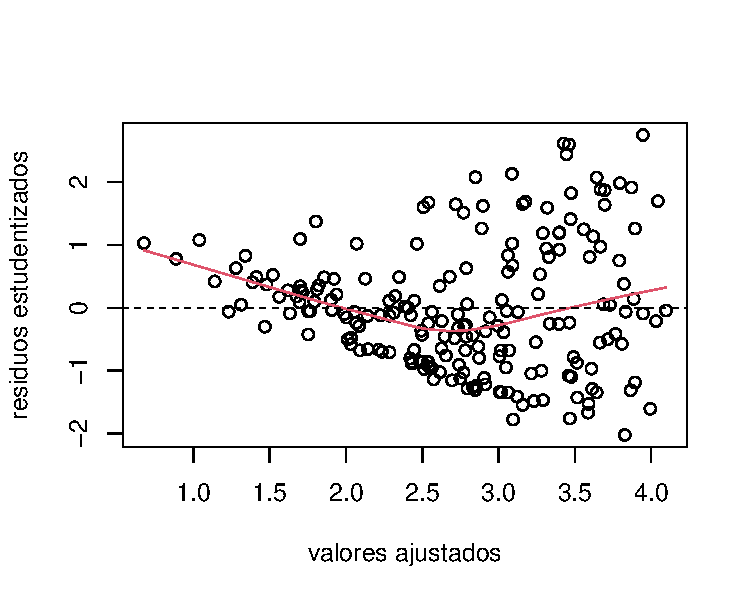
\includegraphics{MLG1_files/figure-latex/Un11res-1} 

}

\caption{Datos de la ONU. Gráfico de los residuos estudentizados.}\label{fig:Un11res}
\end{figure}

\begin{Shaded}
\begin{Highlighting}[]
\FunctionTok{library}\NormalTok{(car)}
\FunctionTok{crPlots}\NormalTok{(mod.UN11,}\AttributeTok{main=}\StringTok{\textquotesingle{}\textquotesingle{}}\NormalTok{)}
\end{Highlighting}
\end{Shaded}

\begin{figure}

{\centering 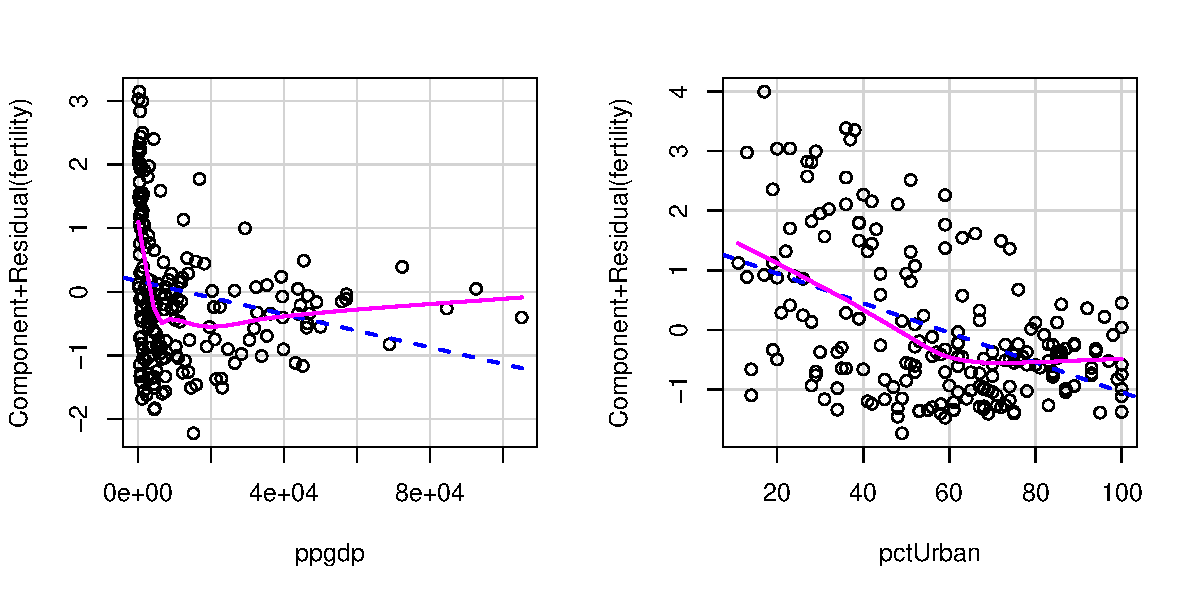
\includegraphics{MLG1_files/figure-latex/Un11resPartial-1} 

}

\caption{Datos de la ONU. Gráfico de los residuos  parciales.}\label{fig:Un11resPartial}
\end{figure}

\hypertarget{ejemplo-2.-datos-de-educaciuxf3n}{%
\subsection*{Ejemplo 2. Datos de educación}\label{ejemplo-2.-datos-de-educaciuxf3n}}
\addcontentsline{toc}{subsection}{Ejemplo 2. Datos de educación}

La base de datos \texttt{education} de la librería \texttt{robustbase} contiene información sobre gastos en educación de 50 estados de los EEUU en el año 1975. Las variables observadas son:

\begin{itemize}
\tightlist
\item
  \textbf{Y}: gasto per cápita en educación pública (dólares, proyectado para 1975).
\item
  \textbf{X1}: número de residentes en áreas urbanas en 1970 (en miles).
\item
  \textbf{X2}: ingreso per cápita en 1973 (en miles dolares).
\item
  \textbf{X3}: número de residentes menores de 18 años en 1974 (en miles)
\end{itemize}

La relación entre las variables se observa en la Figura \ref{fig:Educdata}. Se observa una relación positiva aproximadamente lineal entre la variable respuesta y las covariables, aunque no es tan fuerte con la covariable número de residentes menores de 18 años. Además, vemos que hay por lo menos un posible valor atípico.

\begin{Shaded}
\begin{Highlighting}[]
\FunctionTok{library}\NormalTok{(robustbase)}
\FunctionTok{data}\NormalTok{(}\StringTok{"education"}\NormalTok{)}
\NormalTok{education}\SpecialCharTok{$}\NormalTok{X2 }\OtherTok{=}\NormalTok{ education}\SpecialCharTok{$}\NormalTok{X2}\SpecialCharTok{/}\DecValTok{1000} \CommentTok{\# cambio de unidad de medida (miles de dolares)}
\FunctionTok{pairs}\NormalTok{(education[,}\FunctionTok{c}\NormalTok{(}\DecValTok{6}\NormalTok{,}\DecValTok{3}\SpecialCharTok{:}\DecValTok{5}\NormalTok{)])}
\end{Highlighting}
\end{Shaded}

\begin{figure}

{\centering 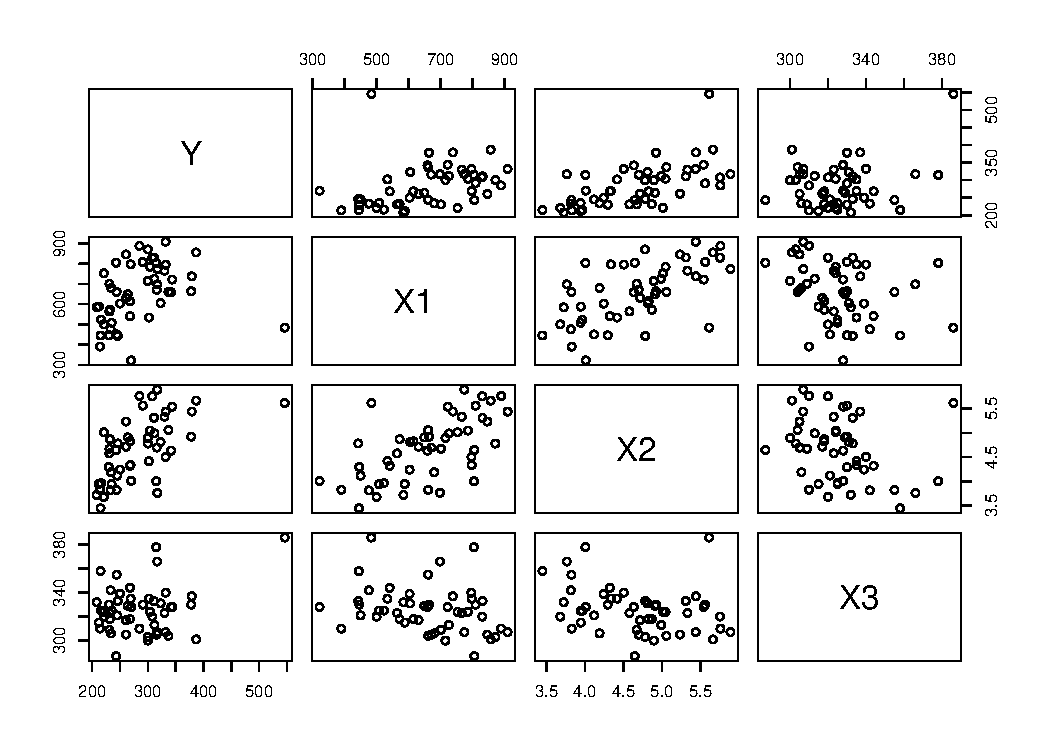
\includegraphics{MLG1_files/figure-latex/Educdata-1} 

}

\caption{Datos de educación. Relación entre las variables.}\label{fig:Educdata}
\end{figure}

El objetivo es ajustar un modelo de regresión para el gasto per cápita en educación pública en función de las demás variables:
\[
Y_{i} = \beta_{0} + \beta_{1}\mbox{X1}_{i} + \beta_{2}\mbox{X2}_{i}+ \beta_{3}\mbox{X3}_{i} + \varepsilon_{i},
\]
donde \(\varepsilon_{i}\sim N(0,\sigma^{2})\) y \(cov(\varepsilon_{j},\varepsilon_{k})=0\).

Antes de hacer inferencias sobre el modelo hacemos un análisis de los residuos. La Figura \ref{fig:Educres} exhibe el gráfico de los residuos estudentizados. Aunque la relación entre la variable respuesta y covariables es aproximadamente lineal, hay presencia de heterocedasticidad. La variabilidad de los residuos aumenta con los valores ajustados.

\begin{Shaded}
\begin{Highlighting}[]
\NormalTok{mod.educ }\OtherTok{=} \FunctionTok{lm}\NormalTok{(Y}\SpecialCharTok{\textasciitilde{}}\NormalTok{X1}\SpecialCharTok{+}\NormalTok{X2}\SpecialCharTok{+}\NormalTok{X3,}\AttributeTok{data=}\NormalTok{education)}
\FunctionTok{library}\NormalTok{(MASS)}
\NormalTok{res.educ }\OtherTok{=} \FunctionTok{studres}\NormalTok{(mod.educ)}
\FunctionTok{par}\NormalTok{(}\AttributeTok{mfrow=}\FunctionTok{c}\NormalTok{(}\DecValTok{1}\NormalTok{,}\DecValTok{2}\NormalTok{))}
\FunctionTok{plot}\NormalTok{(mod.educ}\SpecialCharTok{$}\NormalTok{fitted.values,res.educ,}
     \AttributeTok{xlab=}\StringTok{\textquotesingle{}valores ajustados\textquotesingle{}}\NormalTok{,}\AttributeTok{ylab=}\StringTok{\textquotesingle{}residuos estudentizados\textquotesingle{}}\NormalTok{)}
\FunctionTok{lines}\NormalTok{(}\FunctionTok{lowess}\NormalTok{(res.educ}\SpecialCharTok{\textasciitilde{}}\NormalTok{mod.educ}\SpecialCharTok{$}\NormalTok{fitted.values),}\AttributeTok{col=}\DecValTok{2}\NormalTok{)}
\FunctionTok{abline}\NormalTok{(}\AttributeTok{h=}\DecValTok{0}\NormalTok{,}\AttributeTok{lty=}\DecValTok{2}\NormalTok{)}
\FunctionTok{plot}\NormalTok{(mod.educ}\SpecialCharTok{$}\NormalTok{fitted.values,}\FunctionTok{abs}\NormalTok{(res.educ),}
     \AttributeTok{xlab=}\StringTok{\textquotesingle{}valores ajustados\textquotesingle{}}\NormalTok{,}\AttributeTok{ylab=}\StringTok{\textquotesingle{}| residuos estudentizados |\textquotesingle{}}\NormalTok{)}
\FunctionTok{lines}\NormalTok{(}\FunctionTok{lowess}\NormalTok{(}\FunctionTok{abs}\NormalTok{(res.educ)}\SpecialCharTok{\textasciitilde{}}\NormalTok{mod.educ}\SpecialCharTok{$}\NormalTok{fitted.values),}\AttributeTok{col=}\DecValTok{2}\NormalTok{)}
\end{Highlighting}
\end{Shaded}

\begin{figure}

{\centering 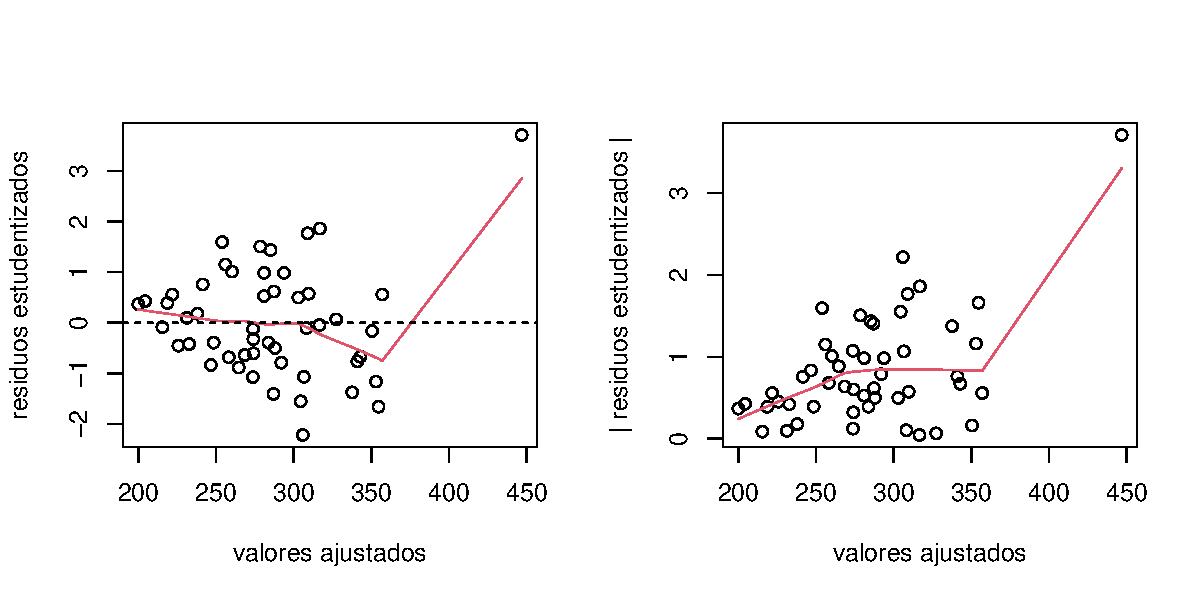
\includegraphics{MLG1_files/figure-latex/Educres-1} 

}

\caption{Datos de educación. Gráficos de los residuos estudentizados.}\label{fig:Educres}
\end{figure}

\rule{\textwidth}{0.4pt}

Dado que los modelos ajustados presentan desviaciones considerables de los supuestos asumidos, las inferencias que se hagan pueden ser invalidas. Por lo tanto, en este capítulo presentaremos dos herramientas para la corrección de estos problemas: (1) transformación de variables (incluyendo la transformación de Box-Cox) y (2) mínimos cuadrados ponderados.

\hypertarget{transformaciuxf3n-de-los-datos}{%
\subsection{Transformación de los datos}\label{transformaciuxf3n-de-los-datos}}

Los objetivos de realizar transformaciones sobre los datos son:

\begin{itemize}
\tightlist
\item
  linealizar la relación de las variables,
\item
  estabilizar la varianza,
\item
  y corregir la normalidad.
\end{itemize}

Las transformaciones pueden hacerse sobre la variable respuesta, las covariables, o ambas.

La desventaja de hacer transformaciones es que la interpretación del modelo estimado, así como las inferencias, se hacen sobre las variables transformadas, y no en su escala original.

\hypertarget{transformaciones-para-linealizar-el-modelo}{%
\subsubsection{Transformaciones para linealizar el modelo}\label{transformaciones-para-linealizar-el-modelo}}

Recordemos que el modelo lineal asume que la relación entre la media y las covariables es aproximadamente lineal. En algunos casos, dada la naturaleza de los datos, este supuesto puede ser violado. Por lo tanto, para seguir utilizando la metodología de los modelos lineales, es posible linealizar funciones no-lineales por medio de transformaciones.

Algunas de estas funciones linealizables y su representación gráfica, se muestran en la Tabla \ref{tab:funciones} y Figura \ref{fig:linealPat}, respectivamente. Por ejemplo, considere que el modelo generador de los datos es:
\[
y_{i} = \beta_{0}\exp\left(\beta_{1}x_{i1} \right)\varepsilon_{i}.
\]
Ver figura \ref{fig:linealPat}(b). Esta relación no lineal se puede linealizar aplicando una transformación logaritmica a ambos lados:

\[
\log y_{i} = y_{i}^{*} = \log \left[ \beta_{0}\exp\left(\beta_{1}x_{i} \right)\varepsilon_{i} \right] = \log \beta_{0} + \beta_{1}x_{i} + \log\varepsilon_{i}.
\]
Note que estaríamos asumiendo que \(\log\varepsilon_{i}\) está normalmente distribuido. Para que esto sea cierto, \(\varepsilon_{i}\) debe seguir una distribución log-normal.

\begin{table}

\caption{\label{tab:funciones}Funciones linealizables}
\centering
\begin{tabular}[t]{llll}
\toprule
 & Función & Transformación & Forma lineal\\
\midrule
(a) & $y = \beta_{0}x^{\beta_{1}}$ & $y^{*}= \log(y), x^{*} = \log(x)$ & $y^{*} =  \log(\beta_{0}) + \beta_{1} x^{*}$\\
(b) & $y = \beta_{0}e^{\beta_{1}x}$ & $y^{*}= \log(y)$ & $y^{*} = \log(\beta_{0}) + \beta_{1} x$\\
(c) & $y = \beta_{0}+\beta_{1}ln(x)$ & $x^{*}= \log(x)$ & $y^{*} = \beta_{0} + \beta_{1} x^{*}$\\
(d) & $y = \frac{x}{\beta_{0}x+\beta_{1}}$ & $x^{*}= \frac{1}{x}, y^{*}= \frac{1}{y}$ & $y^{*} = \beta_{0} - \beta_{1} x^{*}$\\
\bottomrule
\end{tabular}
\end{table}

\begin{figure}

{\centering 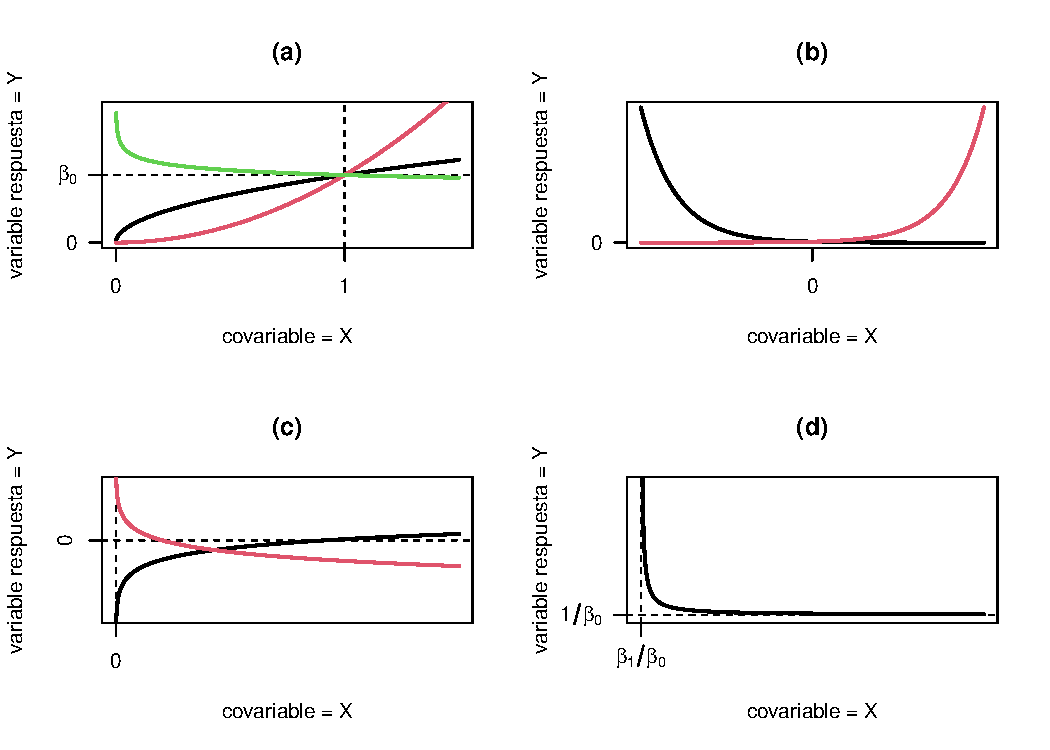
\includegraphics{MLG1_files/figure-latex/linealPat-1} 

}

\caption{Diferentes patrones linealizables.}\label{fig:linealPat}
\end{figure}

\hypertarget{transformaciones-para-estabilizar-la-varianza}{%
\subsubsection{Transformaciones para estabilizar la varianza}\label{transformaciones-para-estabilizar-la-varianza}}

Un caso frecuente es que la variable respuesta sigue una distribución de probabilidad en la que la varianza se relaciona en forma funcional con la media:
\[
V(Y|X=x) = \sigma^2 g[E(Y|X=x)].
\]
Por ejemplo, en la distribución Poisson, la varianza es igual a la media. Algunas transformaciones comunes para estabilizar varianza se muestran en la Tabla \ref{tab:funcionesVar} \citep{behar_validacion_2002}.

\begin{table}

\caption{\label{tab:funcionesVar}Algunas transformaciones para estabilizar la varianza}
\centering
\begin{tabular}[t]{ll}
\toprule
Relación entre $\sigma^{2}$ y $E(Y)$ & Transformación\\
\midrule
$\sigma^{2} \propto C$ & $y^{*}=y$\\
$\sigma^{2} \propto E(y)$ & $y^{*}=\sqrt{y}$\\
$\sigma^{2} \propto E(y)[1-E(y)]$ & $y^{*}=\sin^{-1}\sqrt{y} (0 \leq y_{i} \leq 1)$\\
$\sigma^{2} \propto E(y)^{2}$ & $y^{*}=\log y$  o también  $y^{*}=\log (y+1)$ (si $y \geq 0$)\\
$\sigma^{2} \propto E(y)^{3}$ & $y^{*}=\frac{1}{\sqrt{y}}$\\
\addlinespace
$\sigma^{2} \propto E(y)^{4}$ & $y^{*}=\frac{1}{y}$\\
\bottomrule
\end{tabular}
\end{table}

Algunas consideraciones cuando se hacen transformaciones sobre las variables:

\begin{itemize}
\tightlist
\item
  Transformaciones pueden ser sugeridas por experiencia (o teoría).
  En otros casos, la selección se hace empíricamente.
\item
  Luego de realizar las transformaciones se debe verificar si el modelo transformado cumple los supuestos.
\item
  El estimador de MCO tiene propiedades de mínimos cuadrados con
  respecto a los datos transformados.
\item
  Las predicciones son sobre las respuestas transformadas, no las
  originales. Devolverse a la variable respuesta original no es fácil. Recordemos que
  \[
  E[g(y)] \neq g[E(y)].
  \]
  Al aplicar la transformación inversa a las predicciones de la respuesta transformada estamos estimando la mediana, y no la media. Por otro lado, a las estimaciones por intervalos de confianza si se les puede aplicar la transformación inversa. Esto porque los percentiles no se ven afectados por transformaciones.
\end{itemize}

\rule{\textwidth}{0.4pt}

\hypertarget{datos-de-la-onu.-transformaciuxf3n-para-linealizar-los-datos}{%
\subsubsection*{Datos de la ONU. Transformación para linealizar los datos}\label{datos-de-la-onu.-transformaciuxf3n-para-linealizar-los-datos}}
\addcontentsline{toc}{subsubsection}{Datos de la ONU. Transformación para linealizar los datos}

Al realizar un análisis de residuos del ajuste del modelo para los datos de la ONU, vimos que hay una relación no-lineal entre la fertilidad y las dos covariables propuestas. Particularmente, esto se debe a la covariable producto nacional bruto.

Por lo tanto, podemos aplicar una transformación logarítmica tanto a la variable respuesta, así como la covariable producto nacional bruto. En la Figura \ref{fig:UNtransFig} vemos como al aplicar esta transformación se linealiza la relación.

\begin{figure}

{\centering 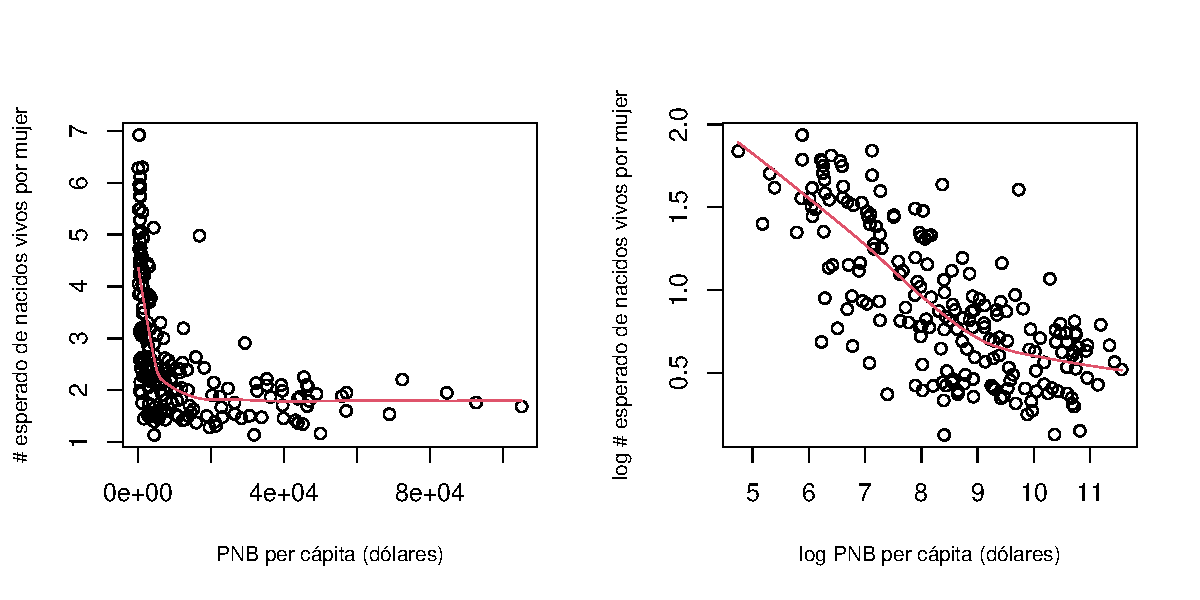
\includegraphics{MLG1_files/figure-latex/UNtransFig-1} 

}

\caption{Datos de la ONU. Relación entre las variables.}\label{fig:UNtransFig}
\end{figure}

Producto de esta transformación, se propone el siguiente modelo:
\[
\log \mbox{fertility}_{i} = \beta_{0} + \beta_{1}\log \mbox{ppgdp}_{i} + \beta_{2}\mbox{pctUrban}_{i} + \varepsilon_{i},
\]
donde \(\varepsilon_{i}\sim N(0,\sigma^{2})\) y \(cov(\varepsilon_{j},\varepsilon_{k})=0\).

La Figura \ref{fig:UNtrans2Fig} muestra el gráfico de los residuos para este ajuste. Aquí vemos que los problemas de no linealidad y heterocedasticidad se corrigieron al realizar la transformación logarítmica.

\begin{Shaded}
\begin{Highlighting}[]
\NormalTok{mod.UN11.trans }\OtherTok{=} \FunctionTok{lm}\NormalTok{(}\FunctionTok{log}\NormalTok{(fertility)}\SpecialCharTok{\textasciitilde{}}\FunctionTok{log}\NormalTok{(ppgdp)}\SpecialCharTok{+}\NormalTok{pctUrban,}\AttributeTok{data =}\NormalTok{ UN11)}
\NormalTok{res.UN11.trans }\OtherTok{=} \FunctionTok{studres}\NormalTok{(mod.UN11.trans)}
\FunctionTok{par}\NormalTok{(}\AttributeTok{mfrow=}\FunctionTok{c}\NormalTok{(}\DecValTok{1}\NormalTok{,}\DecValTok{2}\NormalTok{))}
\FunctionTok{plot}\NormalTok{(mod.UN11.trans}\SpecialCharTok{$}\NormalTok{fitted.values,res.UN11.trans,}\AttributeTok{xlab=}\StringTok{\textquotesingle{}valores ajustados\textquotesingle{}}\NormalTok{,}
     \AttributeTok{ylab=}\StringTok{\textquotesingle{}residuos estudentizados\textquotesingle{}}\NormalTok{)}
\FunctionTok{lines}\NormalTok{(}\FunctionTok{lowess}\NormalTok{(res.UN11.trans}\SpecialCharTok{\textasciitilde{}}\NormalTok{mod.UN11.trans}\SpecialCharTok{$}\NormalTok{fitted.values),}\AttributeTok{col=}\DecValTok{2}\NormalTok{)}
\FunctionTok{abline}\NormalTok{(}\AttributeTok{h=}\DecValTok{0}\NormalTok{,}\AttributeTok{lty=}\DecValTok{2}\NormalTok{)}
\FunctionTok{plot}\NormalTok{(mod.UN11.trans}\SpecialCharTok{$}\NormalTok{fitted.values,}\FunctionTok{abs}\NormalTok{(res.UN11.trans),}\AttributeTok{xlab=}\StringTok{\textquotesingle{}valores ajustados\textquotesingle{}}\NormalTok{,}
     \AttributeTok{ylab=}\StringTok{\textquotesingle{}| residuos estudentizados |\textquotesingle{}}\NormalTok{)}
\FunctionTok{lines}\NormalTok{(}\FunctionTok{lowess}\NormalTok{(}\FunctionTok{abs}\NormalTok{(res.UN11.trans)}\SpecialCharTok{\textasciitilde{}}\NormalTok{mod.UN11.trans}\SpecialCharTok{$}\NormalTok{fitted.values),}\AttributeTok{col=}\DecValTok{2}\NormalTok{)}
\end{Highlighting}
\end{Shaded}

\begin{figure}

{\centering 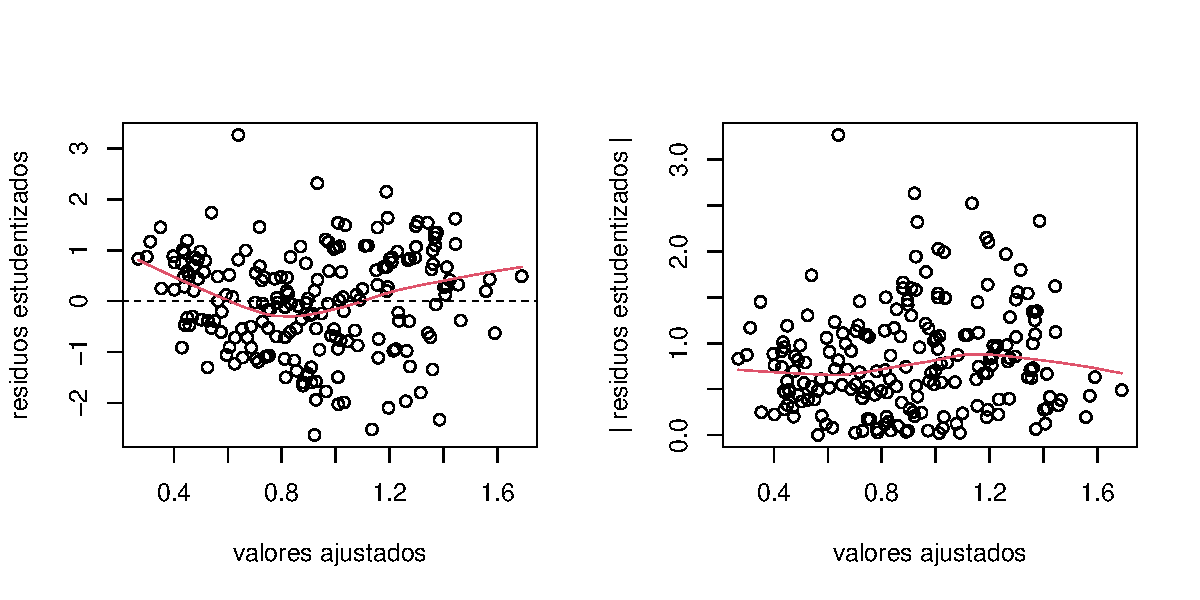
\includegraphics{MLG1_files/figure-latex/UNtrans2Fig-1} 

}

\caption{Datos de la ONU. Gráficos de los residuos para el modelo transformado.}\label{fig:UNtrans2Fig}
\end{figure}
\rule{\textwidth}{0.4pt}

\hypertarget{muxe9todo-de-box-cox}{%
\subsection{Método de Box-Cox}\label{muxe9todo-de-box-cox}}

Para la corrección del supuesto de normalidad y varianza constante, es posible implementar transformaciones en potencia para la variable respuesta. Esto es, \(y^{*}=y^{\lambda}\). Dado que el valor de \(\lambda\) es desconocido, la idea del \textbf{método de Box-Cox} es estimar el modelo lineal para diferentes valores de \(\lambda\) y determinar el valor que proporciona el mejor ajuste. Sin embargo, aquí encontramos dos problemas.

Primero, la transformación en potencia tiene un problema de discontinuidad en \(\lambda=0\). Puesto que cuando \(\lambda\) tiende a cero, \(y^{*}\) se acerca a \(1\). Para resolver esto, se puede utilizar \(y^{*} = (y^{\lambda}-1)/\lambda\). De esta forma, cuando \(\lambda\) tiende a cero, \(y^{*}\) se acerca a \(\log y\). Segundo, cuando \(\lambda\) cambia, los valores \(y^{*}\) varía drásticamente. Esto hace que los modelos ajustados no se puedan comparar fácilmente.

La transformación que permite que los modelos ajustados sean comparables es:
\begin{equation}
y^{(\lambda)} = \begin{cases}
\frac{y^{\lambda}-1}{\lambda \dot{y}^{\lambda-1}}, & \mbox{si }\lambda \neq 0, \\
\dot{y}\log y & \mbox{si } \lambda=0,
\end{cases}
\label{eq:boxcoxtrans}
\end{equation}
donde \(\dot{y} = \log \left[1/n \sum_{i=1}^{n}\log y_{i}\right]\) es la media geométrica de la variable respuesta.

Entonces, el método de Box-Cox es el siguiente:

\begin{enumerate}
\def\labelenumi{\arabic{enumi}.}
\tightlist
\item
  Determinar una secuencia de valores para \(\lambda\), \((\lambda_{1},\lambda_{2},\ldots,\lambda_{K})\). Por lo general, se seleccionan valores en el intervalo \([-2,2]\).
\item
  Ajustar el modelo:
  \[
  y_{ij}^{(\lambda_k)} = \beta_{0} + \beta_{1}x_{i1} + \beta_{2}x_{i2} + \ldots + \beta_{p-1}x_{i,p-1} + \varepsilon_{i},
  \]
  para cada valor de \(\lambda_{k}\), \(k=1,\ldots,K\). Al utilizar la transformación \eqref{eq:boxcoxtrans}, las sumas de cuadrados para modelos con diferentes valores de \(\lambda\) son comparables.
\item
  Seleccionar el modelo que minimiza la suma de cuadrados de los residuos, \(SS_{res}(\lambda)\). Equivalentemente, el \(\lambda\) que maximiza la verosimilitud.
\item
  Luego de encontrar el valor de \(\lambda\) óptimo, se ajusta el modelo transformando la variable respuesta \(y^{\lambda}\), si \(\lambda\neq 0\), o \(\log y\) si \(\lambda =0\). Es decir que (@ref\{eq:boxcoxtrans\}) se utiliza solo en el paso de comparación de modelos ajustados.
\end{enumerate}

Puesto que \(\lambda\) es una variable aleatoria, también se puede hacer una estimación por intervalos de confianza. Para esto primero consideremos la función de log-verosimilitud:
\[
\ell(\boldsymbol \beta,\sigma^{2} | \lambda) = -\frac{2}{n}\log \left( 2\pi\sigma^{2}\right) - \frac{1}{2\sigma^{2}}\sum_{i=1}^{n}\left( y_{i}^{\lambda} - \boldsymbol x_{i}'\boldsymbol \beta\right)^{2} = -\frac{2}{n}\log \left( 2\pi\sigma^{2}\right) - \frac{1}{2\sigma^{2}}SS_{res}(\lambda).
\]
Aquí vemos que el valor de \(\lambda\) que maximiza la verosimilitud es el mismo que minimiza la suma de cuadrados de los residuos.

Un intervalo de confianza se puede construir a partir del siguiente estadístico de prueba:
\[
G_{0}^{2} = -2\left[ \ell(\boldsymbol \beta,\sigma^{2} | \lambda=1) - \ell(\boldsymbol \beta,\sigma^{2} | \lambda=\widehat{\lambda}) \right].
\]
Si \(\lambda=1\), entonces asintóticamente \(G_{0}^{2} \sim \chi^{2}_{1}\). Por lo tanto, el intervalo del \((1-\alpha)\times 100\)\% de confianza para \(\lambda\) está definido por los valores de \(\lambda\) que cumplen con la condición:
\[
 \ell(\boldsymbol \beta,\sigma^{2} | \lambda) \geq  \ell(\boldsymbol \beta,\sigma^{2} | \lambda=\widehat{\lambda}) - \frac{1}{2}\chi^{2}_{1,1-\alpha}.
\]

\rule{\textwidth}{0.4pt}

\hypertarget{datos-de-educaciuxf3n.-transformaciuxf3n-de-box-cox}{%
\subsubsection{Datos de educación. Transformación de Box-Cox}\label{datos-de-educaciuxf3n.-transformaciuxf3n-de-box-cox}}

Dado que el análisis de residuso para el ajuste del modelo para los datos de educación mostró que hay problemas de heterocedasticidad, vamos a encontrar una transformación que resuelva de problema usando el método de Box-Cox. Para esto usamos la función \texttt{boxcox} de la librería \texttt{MASS}:

\begin{Shaded}
\begin{Highlighting}[]
\NormalTok{boxcox.educ }\OtherTok{=}\NormalTok{ MASS}\SpecialCharTok{::}\FunctionTok{boxcox}\NormalTok{(mod.educ,}\AttributeTok{lambda=}\FunctionTok{seq}\NormalTok{(}\SpecialCharTok{{-}}\DecValTok{3}\NormalTok{,}\DecValTok{3}\NormalTok{,}\AttributeTok{length.out =} \DecValTok{1000}\NormalTok{),}
                               \AttributeTok{ylab=}\StringTok{\textquotesingle{}log{-}verosimilitud\textquotesingle{}}\NormalTok{)}
\end{Highlighting}
\end{Shaded}

\begin{figure}

{\centering 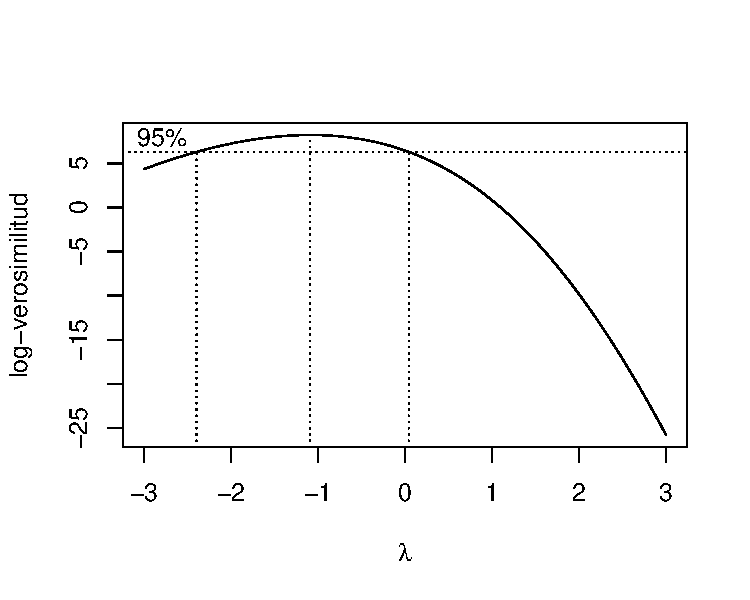
\includegraphics{MLG1_files/figure-latex/educLambda-1} 

}

\caption{\label{fig:EducBC} Datos de educación. Perfiles de verosimilitud para $\lambda$.}\label{fig:educLambda}
\end{figure}

\begin{Shaded}
\begin{Highlighting}[]
\NormalTok{boxcox.educ}\SpecialCharTok{$}\NormalTok{x[boxcox.educ}\SpecialCharTok{$}\NormalTok{y }\SpecialCharTok{==}\FunctionTok{max}\NormalTok{(boxcox.educ}\SpecialCharTok{$}\NormalTok{y)] }\CommentTok{\# valor que maximiza la log{-}verosimilitud}
\end{Highlighting}
\end{Shaded}

\begin{verbatim}
## [1] -1.09009
\end{verbatim}

Estos resultados nos indican que \(\widehat{\lambda}= -1.09\). Por lo cuál, podemos utilizar una transformación inversa \((\lambda=-1)\). Entonces, el modelo propuesto es:
\[
1/y_{i} = \beta_{0} + \beta_{1}\mbox{X1}_{i}+ \beta_{2}\mbox{X2}_{i} + \beta_{3}\mbox{X3}_{i} + \varepsilon_{i},
\]
donde \(\varepsilon_{i}\sim N(0,\sigma^{2})\) y \(cov(\varepsilon_{j},\varepsilon_{k})=0\).

Ahora procedemos a hacer el análisis de los residuos del modelo transformado:

\begin{Shaded}
\begin{Highlighting}[]
\NormalTok{mod.educ.trans }\OtherTok{=} \FunctionTok{lm}\NormalTok{(}\DecValTok{1}\SpecialCharTok{/}\NormalTok{Y}\SpecialCharTok{\textasciitilde{}}\NormalTok{X1}\SpecialCharTok{+}\NormalTok{X2}\SpecialCharTok{+}\NormalTok{X3,}\AttributeTok{data=}\NormalTok{education)}
\NormalTok{res.educ.trans }\OtherTok{=} \FunctionTok{studres}\NormalTok{(mod.educ.trans)}
\FunctionTok{par}\NormalTok{(}\AttributeTok{mfrow=}\FunctionTok{c}\NormalTok{(}\DecValTok{1}\NormalTok{,}\DecValTok{2}\NormalTok{))}
\FunctionTok{plot}\NormalTok{(mod.educ.trans}\SpecialCharTok{$}\NormalTok{fitted.values,res.educ.trans,}
     \AttributeTok{xlab=}\StringTok{\textquotesingle{}valores ajustados\textquotesingle{}}\NormalTok{,}\AttributeTok{ylab=}\StringTok{\textquotesingle{}residuos estudentizados\textquotesingle{}}\NormalTok{)}
\FunctionTok{lines}\NormalTok{(}\FunctionTok{lowess}\NormalTok{(res.educ.trans}\SpecialCharTok{\textasciitilde{}}\NormalTok{mod.educ.trans}\SpecialCharTok{$}\NormalTok{fitted.values),}\AttributeTok{col=}\DecValTok{2}\NormalTok{)}
\FunctionTok{abline}\NormalTok{(}\AttributeTok{h=}\DecValTok{0}\NormalTok{,}\AttributeTok{lty=}\DecValTok{2}\NormalTok{)}
\FunctionTok{plot}\NormalTok{(mod.educ.trans}\SpecialCharTok{$}\NormalTok{fitted.values,}\FunctionTok{abs}\NormalTok{(res.educ.trans),}
     \AttributeTok{xlab=}\StringTok{\textquotesingle{}valores ajustados\textquotesingle{}}\NormalTok{,}\AttributeTok{ylab=}\StringTok{\textquotesingle{}| residuos estudentizados |\textquotesingle{}}\NormalTok{)}
\FunctionTok{lines}\NormalTok{(}\FunctionTok{lowess}\NormalTok{(}\FunctionTok{abs}\NormalTok{(res.educ.trans)}\SpecialCharTok{\textasciitilde{}}\NormalTok{mod.educ.trans}\SpecialCharTok{$}\NormalTok{fitted.values),}\AttributeTok{col=}\DecValTok{2}\NormalTok{)}
\end{Highlighting}
\end{Shaded}

\begin{figure}

{\centering 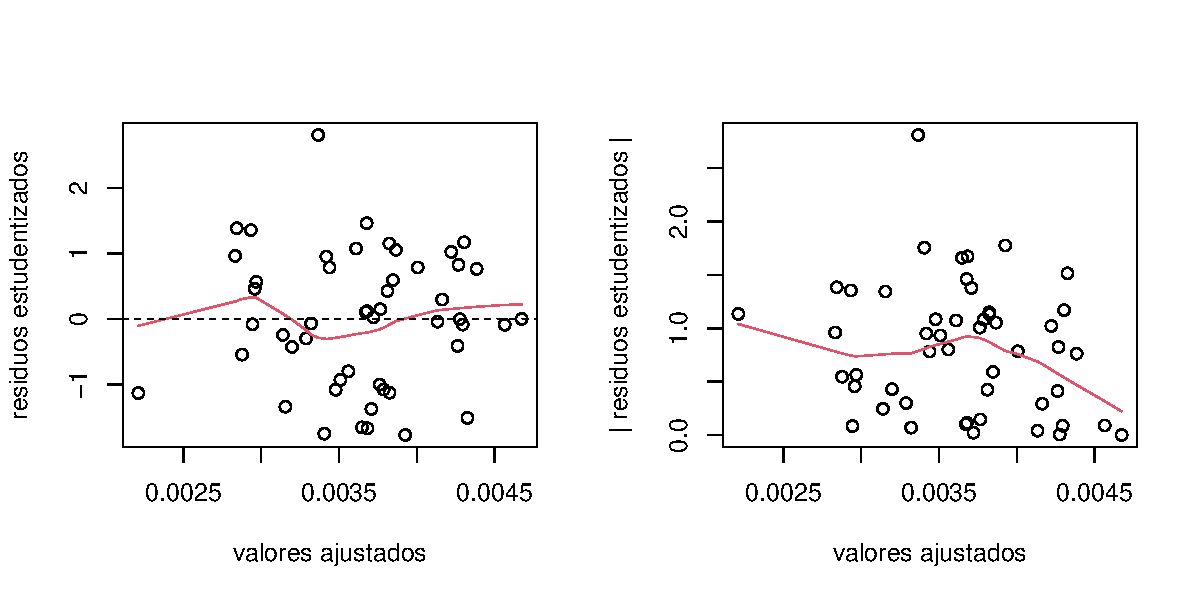
\includegraphics{MLG1_files/figure-latex/EducBC2Fig-1} 

}

\caption{Datos de educación. Graficos de los residuos para el modelo transformado.}\label{fig:EducBC2Fig}
\end{figure}

En la Figura \ref{fig:EducBC2Fig} vemos que la transformación propuesta corrigió el problema de heterocedasticidad. Adicionalmente, por medio de la Figura \ref{fig:EducBC3Fig} podemos verificar que el supuesto de normalidad se cumple.

\begin{Shaded}
\begin{Highlighting}[]
\NormalTok{car}\SpecialCharTok{::}\FunctionTok{qqPlot}\NormalTok{(mod.educ.trans,}\AttributeTok{distribution =} \StringTok{\textquotesingle{}norm\textquotesingle{}}\NormalTok{,}\AttributeTok{ylab=}\StringTok{\textquotesingle{}residuos estudentizados\textquotesingle{}}\NormalTok{)}
\end{Highlighting}
\end{Shaded}

\begin{figure}

{\centering 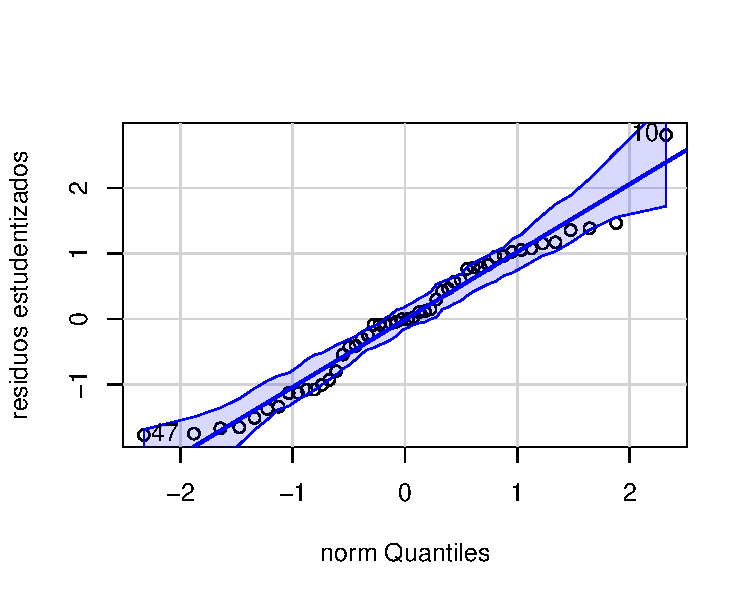
\includegraphics{MLG1_files/figure-latex/EducBC3Fig-1} 

}

\caption{Datos de educación. Graficos de normalidad de los residuos para el modelo transformado.}\label{fig:EducBC3Fig}
\end{figure}

\begin{verbatim}
## [1] 10 47
\end{verbatim}

Puesto que se cumplen los supuestos del modelo transformado, ahora procedemos a interpretar los resultados.

\begin{Shaded}
\begin{Highlighting}[]
\FunctionTok{summary}\NormalTok{(mod.educ.trans)}
\end{Highlighting}
\end{Shaded}

\begin{verbatim}
## 
## Call:
## lm(formula = 1/Y ~ X1 + X2 + X3, data = education)
## 
## Residuals:
##        Min         1Q     Median         3Q        Max 
## -7.609e-04 -3.732e-04 -1.640e-06  3.468e-04  1.158e-03 
## 
## Coefficients:
##               Estimate Std. Error t value Pr(>|t|)    
## (Intercept)  1.220e-02  1.366e-03   8.934 1.29e-11 ***
## X1          -6.613e-07  5.698e-07  -1.161 0.251816    
## X2          -7.302e-04  1.286e-04  -5.676 8.83e-07 ***
## X3          -1.444e-05  3.489e-06  -4.139 0.000147 ***
## ---
## Signif. codes:  0 '***' 0.001 '**' 0.01 '*' 0.05 '.' 0.1 ' ' 1
## 
## Residual standard error: 0.0004487 on 46 degrees of freedom
## Multiple R-squared:  0.5897, Adjusted R-squared:  0.5629 
## F-statistic: 22.04 on 3 and 46 DF,  p-value: 5.417e-09
\end{verbatim}

A partir de estos resultados podemos concluir que la población en áreas urbanas no tiene un aporte signficativo en el modelo cuando las otras dos covariables ya están incluidas. Mientras que, el ingreso per cápita y la población menor de 18 años tienen un efecto positivo significativo sobre el gasto en educación pública (recordemos que se hizo una transformación inversa).

Puesto que hicimos transformaciones, la interpretación de los coeficientes se hace sobre la variable respuesta transformada.

Ahora, supogamos que queremos hacer la predicción del gasto medio en educación pública para los estados que tengan una población de \(\mbox{X1}=650\), un ingreso per cápita de \(\mbox{X2=4.5}\) y una población menor de 18 años de \(\mbox{X3}=320\). A partir del modelo ajustado tenemos que:

\begin{Shaded}
\begin{Highlighting}[]
\NormalTok{x0.educ }\OtherTok{=} \FunctionTok{data.frame}\NormalTok{(}\AttributeTok{X1=}\DecValTok{650}\NormalTok{,}\AttributeTok{X2=}\FloatTok{4.5}\NormalTok{,}\AttributeTok{X3=}\DecValTok{320}\NormalTok{)}
\NormalTok{pred.educ.trans }\OtherTok{=} \FunctionTok{predict}\NormalTok{(mod.educ.trans,x0.educ,}\AttributeTok{interval=}\StringTok{\textquotesingle{}confidence\textquotesingle{}}\NormalTok{) }
\DecValTok{1}\SpecialCharTok{/}\NormalTok{pred.educ.trans}
\end{Highlighting}
\end{Shaded}

\begin{verbatim}
##        fit      lwr      upr
## 1 258.6228 268.5117 249.4364
\end{verbatim}

Por lo que intervalo del 95\% de confianza para el gasto medio en educación pública para los estados con las características expresadas anteriormente es (249.44, 268.51).

\rule{\textwidth}{0.4pt}

\hypertarget{muxednimos-cuadrados-ponderados}{%
\subsection{Mínimos cuadrados ponderados}\label{muxednimos-cuadrados-ponderados}}

El método de mínimos cuadrados ponderados (MCP) es una alternativa para estimar un modelo lineal en presencia de heterocedasticidad. La idea de esta técnica es calcular las desviaciones entre las observaciones \((y_{i})\) y los valores ajustados \((\widehat{y}_{i})\) usando pesos \((w_{i})\) inversamente proporcionales a la varianza de \(y_{i}\).

Asumamos que el modelo generador de los datos es:
\begin{equation}
\boldsymbol y= \boldsymbol X\boldsymbol \beta+ \boldsymbol \varepsilon, \mbox{ donde }\boldsymbol \varepsilon\sim N(\boldsymbol 0,\sigma^{2}\boldsymbol V),
\label{eq:modV}
\end{equation}
donde \(\boldsymbol V\) es una matriz diagonal \((n \times n)\):
\[
\boldsymbol V= \begin{pmatrix}
v_{11} & 0 & 0 & \ldots & 0 \\
0 & v_{22} & 0 & \ldots & 0 \\
0 & 0 & v_{33} & \ldots & 0 \\
\vdots & \vdots & \vdots & \ddots & \vdots \\
0 & 0 & 0 & \ldots & v_{nn}
\end{pmatrix}.
\]
Esto quiere decir que tenemos presencia de hetorocedasticidad, donde \(V(\varepsilon_{i}) = \sigma^{2}v_{ii}\). Recordemos que si aplicamos el estimador por MCO, las estimaciones siguen siendo insesgadas pero son ineficientes. Además, las varianzas estimadas de \(\widehat{\boldsymbol \beta}\), y de las predicciones, están mal calculadas. Lo que puede afectar la cobertura de los intervalos de confianza y el nivel de signficancia de las pruebas de hipótesis.

La función de verosimilitud del modelo \eqref{eq:modV}, asumiendo que \(\boldsymbol V\) es conocida, es:
\[
L(\boldsymbol \beta,\sigma^{2} | \boldsymbol V) =  \frac{1}{(2\pi)^{n/2}|\sigma^{2}\boldsymbol V|^{1/2}}\exp \left[-\frac{1}{2\sigma^{2}}(\boldsymbol y- \boldsymbol X'\boldsymbol \beta)'\boldsymbol V^{-1}(\boldsymbol y- \boldsymbol X'\boldsymbol \beta) \right].
\]
Por lo que para encontrar el estimador de \(\boldsymbol \beta\) debemos minimizar la suma de cuadrados ponderada:
\begin{equation}
SS_{Wres} = (\boldsymbol y- \boldsymbol X'\boldsymbol \beta)'\boldsymbol W(\boldsymbol y- \boldsymbol X'\boldsymbol \beta) = \sum_{i=1}^{n} w_{ii}(y_{i} - \boldsymbol x_{i}'\boldsymbol \beta)^{2},
\label{eq:SSWE}
\end{equation}
donde \(\boldsymbol W= \boldsymbol V^{-1}\), es decir que \(w_{ii}= \frac{1}{v_{ii}}\). Note que las observaciones con mayor varianza tienen menor peso en la estimación de \(\boldsymbol \beta\).

Al minimizar \eqref{eq:SSWE} se obtiene el estimador por MCP:
\[
\widehat{\boldsymbol \beta}_{W} = (\boldsymbol X'\boldsymbol W\boldsymbol X)^{-1}\boldsymbol X'\boldsymbol W\boldsymbol y.
\]
Además,
\begin{equation}
V(\widehat{\boldsymbol \beta}_{W}) = \sigma^{2}(\boldsymbol X'\boldsymbol W\boldsymbol X)^{-1}.
\label{eq:VarBetaW}
\end{equation}
Si \(\boldsymbol V\) está correctamente especificada, se puede probar que \(\widehat{\boldsymbol \beta}_{W}\) es el mejor estimador insesgado de \(\boldsymbol \beta\).

Los residuos del ajuste del modelo son:
\[
e_{Wi} = \sqrt{w_{ii}}(y_{i} - \widehat{y}_{i}), \mbox{ de forma matricial }\boldsymbol e_{W} = \boldsymbol W^{1/2}(\boldsymbol y- \boldsymbol X\widehat{\boldsymbol \beta}_{W}),
\]
donde \(\boldsymbol W= \boldsymbol W^{1/2}\boldsymbol W^{1/2}\). De este resultado obtenemos el estimador insesgado de \(\sigma^{2}\):
\[
\widehat{\sigma}^{2} = \frac{1}{n-p}\sum_{i=1}^{n}w_{ii}(y_{i}-\boldsymbol x_{i}'\widehat{\boldsymbol \beta})^{2} = \frac{1}{n-p}(\boldsymbol y- \boldsymbol X\widehat{\boldsymbol \beta})'\boldsymbol W(\boldsymbol y- \boldsymbol X\widehat{\boldsymbol \beta}).
\]

Aqui estamos asumiendo que los pesos \((w_{ii})\) son conocidos. Lo que en la práctica es poco común. Estos pesos pueden ser determinados por conocimiento de los datos, experiencia, o información teórica del modelo. Alternativamente, estos se pueden calcular a partir de los residuos obtenidos por el estimador MCO.

Es común que \(\sigma^{2}_{i}\) varíe de acuerdo a una o varias covariables, o con respecto \(E(y_{i}|\boldsymbol x_{i})\). Por ejemplo, en los datos de educación parece que la varianza incrementa con \(E(y_{i}| \boldsymbol x_{i})\). En este caso podemos aplicar el siguiente procedimiento:

\begin{enumerate}
\def\labelenumi{\arabic{enumi}.}
\tightlist
\item
  Ajustar el modelo por MCO y analizar los residuos.
\item
  Ajustar un modelo para el valor absoluto de los residuos \((|e_{i}|)\), o los residuso al cuadrado \((e^{2}_{i})\), en función de las covariables:
  \[
  |e_{i}| = \gamma_{0} + \gamma_{1}x_{i1}+ \ldots + \gamma_{p-1}x_{i,p-1} + \varepsilon_{ei}.
  \]
  De esta ajuste obtenemos una estimación para la desviación estándar \((\sigma_{i})\). Si ajustamos un modelo para los residuos al cuadrado, estamos estimando la varianza \((\sigma^{2})\).
\item
  Usar los valores ajustados el modelo anterior para estimar los pesos \((w_{ii})\).
\end{enumerate}

Si \(\widehat{\boldsymbol \beta}_{W}\) difiere mucho de \(\widehat{\boldsymbol \beta}\), es posible repetir el proceso anterior una vez más (mínimos cuadrados iterativamente ponderados).

Dado que estamos estimando los pesos, la varianza de los coeficientes \eqref{eq:VarBetaW} es aproximada. Sin embargo, esta aproximación es muy buena si el tamaño de muestra no es muy pequeño.

\rule{\textwidth}{0.4pt}

\hypertarget{datos-de-educaciuxf3n.-minuxedmos-cuadrados-ponderados}{%
\subsubsection*{Datos de educación. Minímos cuadrados ponderados}\label{datos-de-educaciuxf3n.-minuxedmos-cuadrados-ponderados}}
\addcontentsline{toc}{subsubsection}{Datos de educación. Minímos cuadrados ponderados}

Retomemos el modelo para los datos de educación. En la Figura @ref\{fig:Educres\} vemos que hay heterocedasticidad. Particularmente vemos que la variabilidad crece a medida que aumentan los valores ajustados. Ya vimos que por medio de una transformación inversa sobre la variable respuesta se corrige el problema.

El problema de hacer transformaciones es que los coeficientes estimados pierden interpretación. Así que, alternativamente, vamos a implementar el método de minímos cuadrados ponderados. Dado que desconocemos los pesos, vamos a estimarlos usando el procedimiento que se explicó anteriormente.

Primero vamos a ajustar el siguiente modelo para el valor absoluto de los residuos:
\[
|e_{i}| = \gamma_{0} + \gamma_{1}\mbox{X1}_{i}+ \gamma_{2}\mbox{X2}_{i} + \gamma_{3}\mbox{X3}_{i} + \varepsilon_{ei}.
\]

\begin{Shaded}
\begin{Highlighting}[]
\NormalTok{mod.stdev.educ }\OtherTok{=} \FunctionTok{lm}\NormalTok{(}\FunctionTok{abs}\NormalTok{(res.educ)}\SpecialCharTok{\textasciitilde{}}\NormalTok{X1}\SpecialCharTok{+}\NormalTok{X2}\SpecialCharTok{+}\NormalTok{X3,}\AttributeTok{data =}\NormalTok{ education)}
\FunctionTok{summary}\NormalTok{(mod.stdev.educ)}
\end{Highlighting}
\end{Shaded}

\begin{verbatim}
## 
## Call:
## lm(formula = abs(res.educ) ~ X1 + X2 + X3, data = education)
## 
## Residuals:
##      Min       1Q   Median       3Q      Max 
## -1.23416 -0.38164 -0.00938  0.32668  1.37892 
## 
## Coefficients:
##               Estimate Std. Error t value Pr(>|t|)    
## (Intercept) -4.6137734  1.7454477  -2.643   0.0112 *  
## X1          -0.0014511  0.0007281  -1.993   0.0522 .  
## X2           0.7274821  0.1643850   4.425 5.87e-05 ***
## X3           0.0092325  0.0044583   2.071   0.0440 *  
## ---
## Signif. codes:  0 '***' 0.001 '**' 0.01 '*' 0.05 '.' 0.1 ' ' 1
## 
## Residual standard error: 0.5734 on 46 degrees of freedom
## Multiple R-squared:  0.3199, Adjusted R-squared:  0.2756 
## F-statistic: 7.214 on 3 and 46 DF,  p-value: 0.0004565
\end{verbatim}

Por lo tanto, las estimaciones de las desviaciones estándar de los errores son:
\[
\widetilde{\sigma}_{i} = s_{i} = -4.614  -0.001\mbox{X1}_{i} + 0.727\mbox{X2}_{i} + 0.009\mbox{X3}_{i}.
\]
De este ajuste obtenemos los pesos \(w_{ii} = \frac{1}{s_{i}^{2}}\), y luego, estimamos el modelo por MCP:

\begin{Shaded}
\begin{Highlighting}[]
\NormalTok{w }\OtherTok{=} \DecValTok{1}\SpecialCharTok{/}\NormalTok{mod.stdev.educ}\SpecialCharTok{$}\NormalTok{fitted.values}\SpecialCharTok{\^{}}\DecValTok{2}
\NormalTok{mod.educ.mcp }\OtherTok{=} \FunctionTok{lm}\NormalTok{(Y}\SpecialCharTok{\textasciitilde{}}\NormalTok{X1}\SpecialCharTok{+}\NormalTok{X2}\SpecialCharTok{+}\NormalTok{X3,}\AttributeTok{data=}\NormalTok{education,}\AttributeTok{weights =}\NormalTok{ w)}
\FunctionTok{summary}\NormalTok{(mod.educ.mcp)}
\end{Highlighting}
\end{Shaded}

\begin{verbatim}
## 
## Call:
## lm(formula = Y ~ X1 + X2 + X3, data = education, weights = w)
## 
## Weighted Residuals:
##     Min      1Q  Median      3Q     Max 
## -93.670 -32.522  -9.149  31.582  86.742 
## 
## Coefficients:
##               Estimate Std. Error t value Pr(>|t|)    
## (Intercept) -404.85597   84.79548  -4.774 1.87e-05 ***
## X1             0.05062    0.03778   1.340    0.187    
## X2            62.43586   10.29479   6.065 2.32e-07 ***
## X3             1.11736    0.20099   5.559 1.32e-06 ***
## ---
## Signif. codes:  0 '***' 0.001 '**' 0.01 '*' 0.05 '.' 0.1 ' ' 1
## 
## Residual standard error: 44.98 on 46 degrees of freedom
## Multiple R-squared:  0.6528, Adjusted R-squared:  0.6302 
## F-statistic: 28.83 on 3 and 46 DF,  p-value: 1.219e-10
\end{verbatim}

La Figura \ref{fig:EducMCPFig} muestra los gráficos de los residuos ponderados. Aquí podemos observar que los residuos ponderados no muestra heterocedasticidad.

\begin{Shaded}
\begin{Highlighting}[]
\NormalTok{res.educ.mcp }\OtherTok{=}\NormalTok{ mod.educ.mcp}\SpecialCharTok{$}\NormalTok{residuals}\SpecialCharTok{*}\FunctionTok{sqrt}\NormalTok{(w)}
\FunctionTok{par}\NormalTok{(}\AttributeTok{mfrow=}\FunctionTok{c}\NormalTok{(}\DecValTok{1}\NormalTok{,}\DecValTok{2}\NormalTok{))}
\FunctionTok{plot}\NormalTok{(mod.educ.mcp}\SpecialCharTok{$}\NormalTok{fitted.values,res.educ.mcp,}
     \AttributeTok{xlab=}\StringTok{\textquotesingle{}valores ajustados\textquotesingle{}}\NormalTok{,}\AttributeTok{ylab=}\StringTok{\textquotesingle{}residuos ponderados\textquotesingle{}}\NormalTok{)}
\FunctionTok{lines}\NormalTok{(}\FunctionTok{lowess}\NormalTok{(res.educ.mcp}\SpecialCharTok{\textasciitilde{}}\NormalTok{mod.educ.mcp}\SpecialCharTok{$}\NormalTok{fitted.values),}\AttributeTok{col=}\DecValTok{2}\NormalTok{)}
\FunctionTok{abline}\NormalTok{(}\AttributeTok{h=}\DecValTok{0}\NormalTok{,}\AttributeTok{lty=}\DecValTok{2}\NormalTok{)}
\FunctionTok{plot}\NormalTok{(mod.educ.mcp}\SpecialCharTok{$}\NormalTok{fitted.values,}\FunctionTok{abs}\NormalTok{(res.educ.mcp),}
     \AttributeTok{xlab=}\StringTok{\textquotesingle{}valores ajustados\textquotesingle{}}\NormalTok{,}\AttributeTok{ylab=}\StringTok{\textquotesingle{}| residuos ponderados |\textquotesingle{}}\NormalTok{)}
\FunctionTok{lines}\NormalTok{(}\FunctionTok{lowess}\NormalTok{(}\FunctionTok{abs}\NormalTok{(res.educ.mcp)}\SpecialCharTok{\textasciitilde{}}\NormalTok{mod.educ.mcp}\SpecialCharTok{$}\NormalTok{fitted.values),}\AttributeTok{col=}\DecValTok{2}\NormalTok{)}
\end{Highlighting}
\end{Shaded}

\begin{figure}

{\centering 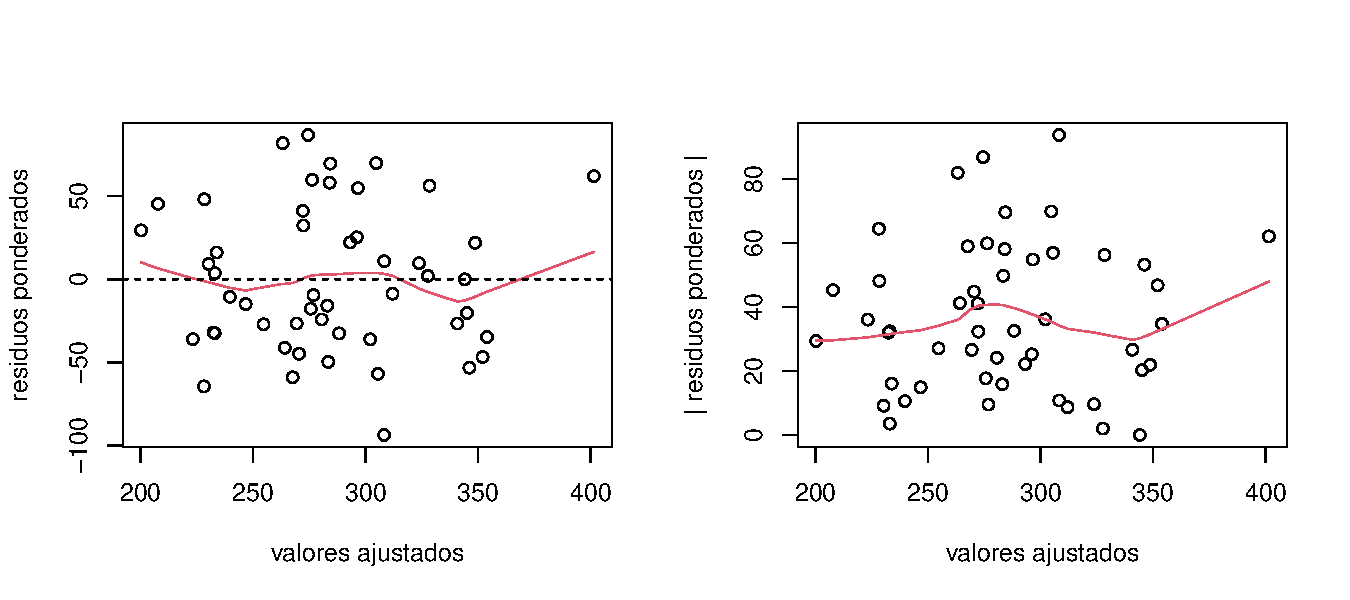
\includegraphics{MLG1_files/figure-latex/EducMCPFig-1} 

}

\caption{Datos de educación. Graficos de los residuos ponderados.}\label{fig:EducMCPFig}
\end{figure}

El ajuste por mínimos cuadrados ponderados es:

\begin{Shaded}
\begin{Highlighting}[]
\FunctionTok{summary}\NormalTok{(mod.educ.mcp)}
\end{Highlighting}
\end{Shaded}

\begin{verbatim}
## 
## Call:
## lm(formula = Y ~ X1 + X2 + X3, data = education, weights = w)
## 
## Weighted Residuals:
##     Min      1Q  Median      3Q     Max 
## -93.670 -32.522  -9.149  31.582  86.742 
## 
## Coefficients:
##               Estimate Std. Error t value Pr(>|t|)    
## (Intercept) -404.85597   84.79548  -4.774 1.87e-05 ***
## X1             0.05062    0.03778   1.340    0.187    
## X2            62.43586   10.29479   6.065 2.32e-07 ***
## X3             1.11736    0.20099   5.559 1.32e-06 ***
## ---
## Signif. codes:  0 '***' 0.001 '**' 0.01 '*' 0.05 '.' 0.1 ' ' 1
## 
## Residual standard error: 44.98 on 46 degrees of freedom
## Multiple R-squared:  0.6528, Adjusted R-squared:  0.6302 
## F-statistic: 28.83 on 3 and 46 DF,  p-value: 1.219e-10
\end{verbatim}

Aquí llegamos a conclusiones similares a las obtenidas por medio del modelo transformado. El efecto de la población en áreas urbanas no es significativo. Las otras dos covariables si aportan significativamente al modelo. En este caso, dado que no aplicamos transformaciones, los coeficientes si tienen interpretación. Por ejemplo de la estimación de \(\beta_{3}\) podemos concluir que: el gasto per cápita medio en educación pública aumenta en 1.117 USD por cada 1000 personas menores de 18 años.

Ahora, hagamos la predicción del gasto medio en educación pública para las características: \(\mbox{X1}=650\), \(\mbox{X2=4.5}\) y \(\mbox{X3}=320\):

\begin{Shaded}
\begin{Highlighting}[]
\FunctionTok{predict}\NormalTok{(mod.educ.mcp,x0.educ,}\AttributeTok{interval=}\StringTok{\textquotesingle{}confidence\textquotesingle{}}\NormalTok{)}
\end{Highlighting}
\end{Shaded}

\begin{verbatim}
##        fit      lwr      upr
## 1 266.5599 257.8442 275.2755
\end{verbatim}

Por medio del estimador de MCP obtenemos el siguiente intervalo del 95\% de confianza: (257.844, 275.275). Este intervalo es parecido al calculado usando el modelo transformado, aunque tiene una longitud un poco más pequeña.

\hypertarget{evaluaciuxf3n-de-puntos-influyentes-y-atuxedpicos}{%
\section{Evaluación de puntos influyentes y atípicos}\label{evaluaciuxf3n-de-puntos-influyentes-y-atuxedpicos}}

\rule{\textwidth}{0.4pt}

\hypertarget{datos-de-la-onu}{%
\subsection{Datos de la ONU}\label{datos-de-la-onu}}

Retomemos los datos de la ONU (\texttt{UN11} de la librería \texttt{alr4}). El modelo propuesto es:
\begin{equation}
\log \mbox{fertility}_{i} = \beta_{0} + \log \mbox{ppgdp}_{i}\beta_{1} + \mbox{pctUrban}_{i}\beta_{2} + \varepsilon_{i},
\label{eq:modUN}
\end{equation}
donde \(\varepsilon_{i}\sim N(0,\sigma^{2})\) y \(cov(\varepsilon_{j},\varepsilon_{k})=0\).

El análisis de los residuos (ver Figura \ref{fig:Un11resFig}) muestra que el modelo está bien especificado y no hay problemas de heterocedasticidad. Sin embargo, podemos observar que algunos residuos presentan valores muy altos. La estimación de la \(\log \mbox{fertility}\) para Guinea Ecuatorial es considerablemente baja en comparación con el valor observado. Caso contrario pasa con Corea del Norte, Bosnia y Herzegovina, y Moldavia.

\begin{figure}

{\centering 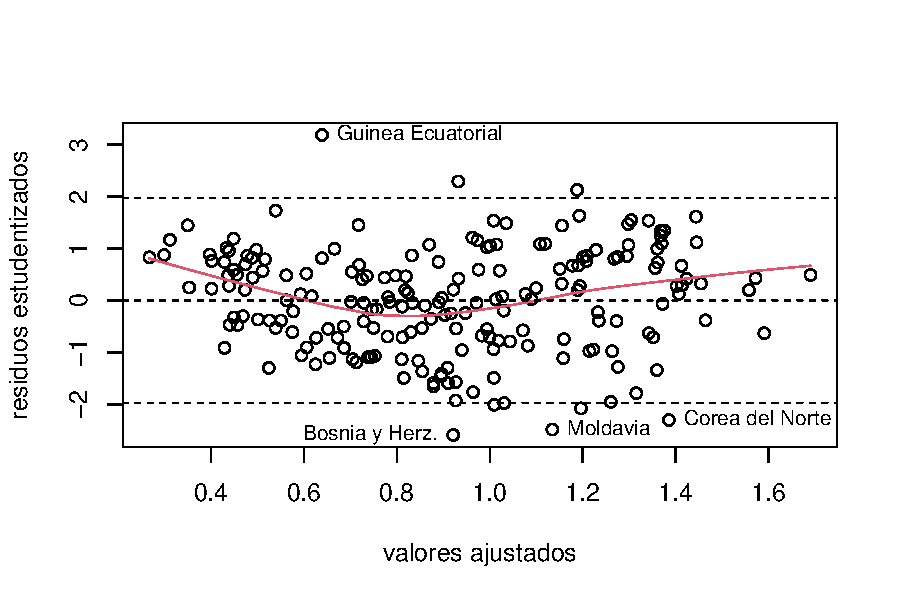
\includegraphics{MLG1_files/figure-latex/Un11resFig-1} 

}

\caption{Datos de la ONU. Gráfico de los residuos estudentizados.}\label{fig:Un11resFig}
\end{figure}
\rule{\textwidth}{0.4pt}

\hypertarget{importancia-de-detectar-valores-influyentes-y-atuxedpicos}{%
\subsection{Importancia de detectar valores influyentes y atípicos}\label{importancia-de-detectar-valores-influyentes-y-atuxedpicos}}

En el análisis de datos pueden observarse algunos valores atípicos. Como atípicas nos referimos a las observaciones que no siguen el patrón de la mayoría de los datos. En un análisis de regresión, pueden presentarse valores atípicos sobre la variable respuesta y/o sobre algunas covariables. Por lo tanto, se podría identificar diferentes tipos de puntos ``atípicos'\,'. Estos se pueden identificar en la Figura \ref{fig:puntosAI} para el caso de una regresión simple:

\begin{itemize}
\tightlist
\item
  \textbf{\(A\) es un punto atípico:} valor que no se ajusta bien en \(Y\), pero regular en \(X\).
\item
  \textbf{\(B\) es un punto de balanceo:} observación que se ajusta bien en \(Y\), pero es inusual en \(X\).
\item
  \textbf{\(C\) es un punto de influyente:} medición que no se ajusta bien en \(Y\) y es inusual en \(X\).
\end{itemize}

Estos puntos inusuales pueden ser problemáticos a la hora de ajustar un modelo lineal por MCO, ya que pueden tener mucha influencia en los resultados, y su presencia puede ser una señal de que el modelo no captura caraterísticas importantes de los datos.

\begin{figure}

{\centering 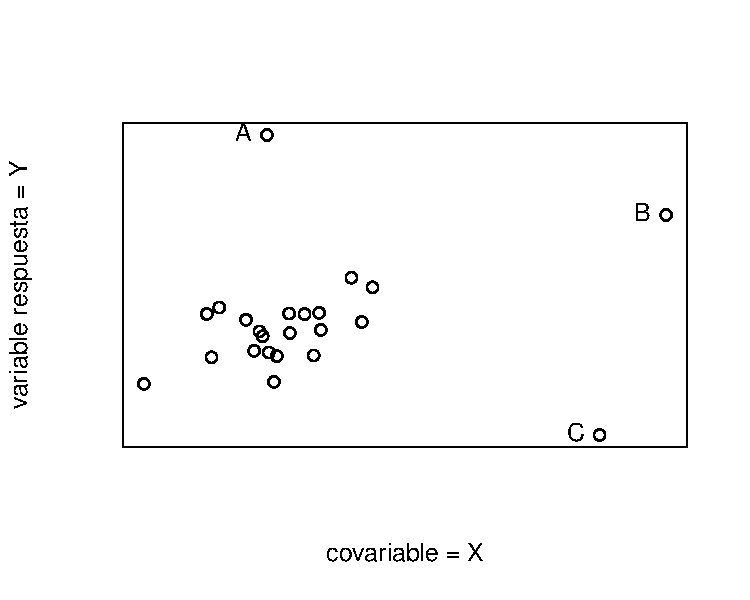
\includegraphics{MLG1_files/figure-latex/puntosAI-1} 

}

\caption{Diferentes tipos de datos. A: Punto atípico, B: punto de balanceo, C: punto influyente.}\label{fig:puntosAI}
\end{figure}

En la Figura \ref{fig:puntosAIw}(a) vemos que un punto atípico no tiene un efecto grande en la estimación de la recta de regresión. Sin embargo, dado que los puntos atípicos generan valores altos (en valor absoluto) para los residuos, estas observaciones inflan la varianza de las estimaciones y afectan las inferencias. En este caso, la estimación de la varianza con todos los datos es de \(\widehat{\sigma}^{2}=6.37\), y si se omite el dato \(A\), tenemos que \(\widehat{\sigma}^{2}=1.55\). Como vemos en la Figura @ref\{fig:puntosAIw\}(b) los puntos de balanceo tampoco tienen mucha influencia sobre las estimaciones por MCO ya que estos están en línea con el resto de los datos.

Por el otro lado, en la Figura \ref{fig:puntosAIw}(c) vemos que los puntos influyentes afectan notablemente las estimaciones por MCO. Además, también inflan considerablemente la variabilidad. Con todos los datos tenemos que \(\widehat{\sigma}^{2}=3.09\). Mientras que \(\widehat{\sigma}^{2}=1.55\) al eliminar la observación C.

\begin{figure}

{\centering 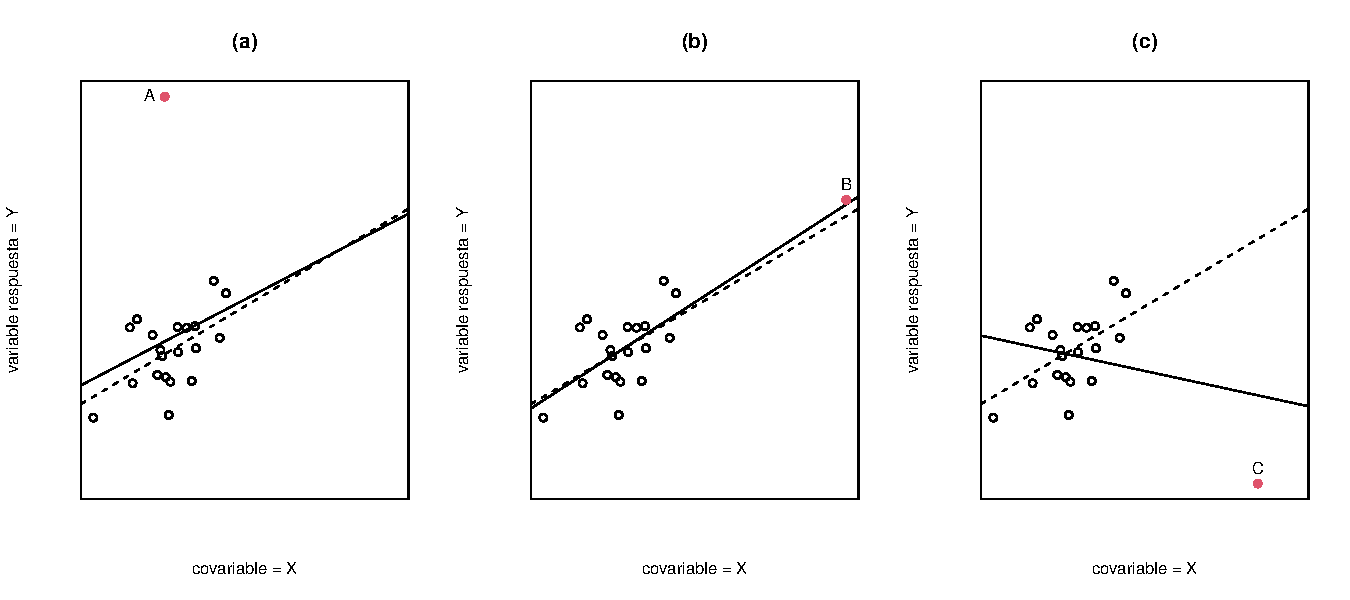
\includegraphics{MLG1_files/figure-latex/puntosAIw-1} 

}

\caption{Efecto de los puntos inusuales. En cada gráfico, la línea continua es la estimación por MCO con todos los datos, mientras que la línea discontinua es la estimación por MCO omitiendo el punto inusual (circulo rojo). Izquierda: efecto de un punto atípico. Centro: efecto de un punto de balanceo. Derecha: efecto de un punto influyente.}\label{fig:puntosAIw}
\end{figure}

\hypertarget{valores-atuxedpicos}{%
\subsection{Valores atípicos}\label{valores-atuxedpicos}}

Para identificar valores atípicos podemos hacer uso de los residuos del ajuste. Recordemos que, aunque los errores tenga varianza constante y sean incorrelacionados, los residuos no cumplen con estas propiedades. Por lo tanto, es recomendado usar los residuos estudentizados (o los residuos R-Student):
\[
r_{i} = \frac{e_{i}}{\sqrt{\widehat{\sigma}^{2}(1-h_{ii})}}, i=1,\ldots,n,
\]
o los residuos R-Student:
\[
t_{i} = \frac{e_{i}}{\sqrt{\widehat{\sigma}^{2}_{(i)}(1-h_{ii})}} = r_{i} \sqrt{\frac{n-p-1}{n-p-r_{i}^{2}}},
\]
donde \(\widehat{\sigma}^{2}_{(i)}\) es la estimación de \(\sigma\) usando todas las observaciones excepto la \(i\)-ésima.

Si se cumplen los supuestos del modelo, se puede demostrar que \(r_{i}\sim t_{n-p-1}\). Los residuos estudentizados siguen también está distribución pero de forma aproximada. Por lo tanto, se pueden identificar posibles valores atípicos haciendo un gráfico de los R-Student (o residuos estudentizados) contra los valores ajustados y trazar líneas de referencia en los percentiles \(0.025\) y \(0.975\) de la distribución \(t\) con \(n-p-1\) grados de libertad.

Esta verificación no es estrictamente una prueba de hipótesis. Puesto que estamos haciendo múltiplescomparaciones de los residuos R-Student con los valores criticos de la distribución \(t\). Por lo que es necesario hacer una corrección utilizando el método de Bonferroni.

\rule{\textwidth}{0.4pt}

\hypertarget{datos-de-la-onu---valores-atuxedpicos}{%
\subsubsection*{Datos de la ONU - valores atípicos}\label{datos-de-la-onu---valores-atuxedpicos}}
\addcontentsline{toc}{subsubsection}{Datos de la ONU - valores atípicos}

En la Figura \ref{fig:Un11res} podemos observar que hay varios residuos que sobrepasan los puntos de corte. Particularmente, la observación de Guinea Ecuatorial presenta un residuo muy alto.

\rule{\textwidth}{0.4pt}

\hypertarget{puntos-de-balanceo}{%
\subsection{Puntos de balanceo}\label{puntos-de-balanceo}}

Recordemos que la estimación de la recta de regresión es un promedio ponderado de las observaciones:
\[
\widehat{\boldsymbol y}= \boldsymbol X\widehat{\boldsymbol \beta}= \boldsymbol X(\boldsymbol X'\boldsymbol X)^{-1}\boldsymbol X'\boldsymbol y= \boldsymbol H\boldsymbol y.
\]
Para la observación \(y_{i}\) tenemos que \(\widehat{y}_{i} = h_{ii}y_{i} + \sum_{k\neq i}h_{ik}y_{j}\). Particularmente, el elemento \(h_{ij}\) pueden ser visto como la cantidad de balanceo o palanqueo ejercido por la j-ésima observación \((y_i)\) sobre el \(i\)-ésimo valor ajustado (\(\widehat{y}_{i}\)).

Entonces, para detectar valores influyentes vamos a centrarnos en la matriz \textit{hat} \((\boldsymbol H)\). El elemento \(h_{ij}\) de esta matriz se calcula como:
\begin{equation}
h_{ij} = \boldsymbol x_{i}'(\boldsymbol X'\boldsymbol X)\boldsymbol x_{j}.
\label{eq:hij}
\end{equation}
Algunas propiedades de la matriz \(\boldsymbol H\) son:

\begin{itemize}
\item $\sum_{i=1}^{n} = p$.
\item $\sum_{i=1}^{n}h_{ij} = \sum_{j=1}^{n}h_{ij} = 1$
\item Cada valor $h_{ii}$ está acotado entre $1/n$ y $1/r$ ($r$ es el número de columnas de $\boldsymbol X$ iguales a $\boldsymbol x_{i}$).
\end{itemize}

Además, la diagonal de la matriz \(\boldsymbol H\) es una medida estandarizada de la distancia de las observaciones al centro (centroide) del espacio de \(\boldsymbol x\). Por lo tanto, valores altos en la diagonal de \(\boldsymbol H\) pueden indicarnos observaciones que son potencialmente influyentes porque están alejadas en el espacio de las covariables. Viendo \eqref{eq:hij}, si \(h_{ii}\) es muy cercano a uno, \(\widehat{y}_{i}\) estará muy cerca de \(y_{i}\) (dado que el peso de las demás observaciones será casi cero).

Dado que \(\bar{h} = p/n\), observaciones con \(h_{ii}\) superiores a \(2p/n\) son considerados \textbf{puntos de balanceo} (y posibles puntos influyentes). Note que, si \(2p/n > 1\), el punto de corte no aplica.

\rule{\textwidth}{0.4pt}

\hypertarget{datos-de-la-onu---diagonal-de-la-matrix-hat}{%
\subsubsection*{Datos de la ONU - diagonal de la matrix hat}\label{datos-de-la-onu---diagonal-de-la-matrix-hat}}
\addcontentsline{toc}{subsubsection}{Datos de la ONU - diagonal de la matrix hat}

La Figura \ref{fig:Un11Hdiag}(a) muestra los valores de la diagonal de la matrix \(\boldsymbol H\). Aquí podemos observar que algunos países presentan valores más altos del punto de corte (\(2\frac{p}{n} = 0.0302\)). Comparado con los demás valores, el valor asociado a Trinidad y Tobago es muy alto. Por lo cuál este país lo podemos considerar como un punto de balanceo.

\begin{Shaded}
\begin{Highlighting}[]
\FunctionTok{library}\NormalTok{(alr4)}
\FunctionTok{data}\NormalTok{(UN11)}
\NormalTok{Names }\OtherTok{=} \FunctionTok{rownames}\NormalTok{(UN11)}
\NormalTok{mod.UN11 }\OtherTok{=} \FunctionTok{lm}\NormalTok{(}\FunctionTok{log}\NormalTok{(fertility)}\SpecialCharTok{\textasciitilde{}}\FunctionTok{log}\NormalTok{(ppgdp)}\SpecialCharTok{+}\NormalTok{pctUrban,}\AttributeTok{data=}\NormalTok{UN11)}
\NormalTok{hii }\OtherTok{=} \FunctionTok{hatvalues}\NormalTok{(mod.UN11)}
\FunctionTok{par}\NormalTok{(}\AttributeTok{mfrow=}\FunctionTok{c}\NormalTok{(}\DecValTok{1}\NormalTok{,}\DecValTok{2}\NormalTok{))}
\FunctionTok{plot}\NormalTok{(hii,}\AttributeTok{type=}\StringTok{\textquotesingle{}h\textquotesingle{}}\NormalTok{,}\AttributeTok{xlab=}\StringTok{\textquotesingle{}índice\textquotesingle{}}\NormalTok{,}\AttributeTok{ylab=}\StringTok{\textquotesingle{}valores de la diagonal de la matrix hat\textquotesingle{}}\NormalTok{)}
\FunctionTok{abline}\NormalTok{(}\AttributeTok{h=}\DecValTok{2}\SpecialCharTok{*}\DecValTok{3}\SpecialCharTok{/}\DecValTok{199}\NormalTok{,}\AttributeTok{lty=}\DecValTok{2}\NormalTok{)}
\NormalTok{hii[hii}\SpecialCharTok{\textgreater{}}\DecValTok{2}\SpecialCharTok{*}\DecValTok{3}\SpecialCharTok{/}\DecValTok{199}\NormalTok{]}
\end{Highlighting}
\end{Shaded}

\begin{verbatim}
##            Djibouti             Liberia               Nauru         North Korea 
##          0.03105290          0.03747901          0.03708513          0.03105839 
##             Somalia           Sri Lanka Trinidad and Tobago 
##          0.04390710          0.03334886          0.07590435
\end{verbatim}

\begin{Shaded}
\begin{Highlighting}[]
\FunctionTok{plot}\NormalTok{(}\FunctionTok{log}\NormalTok{(UN11}\SpecialCharTok{$}\NormalTok{ppgdp),UN11}\SpecialCharTok{$}\NormalTok{pctUrban,}\AttributeTok{xlab=}\StringTok{\textquotesingle{}log del PNB per cápita\textquotesingle{}}\NormalTok{,}
     \AttributeTok{ylab=}\StringTok{\textquotesingle{}\% de población urbanas\textquotesingle{}}\NormalTok{)}
\FunctionTok{points}\NormalTok{(}\FunctionTok{log}\NormalTok{(UN11}\SpecialCharTok{$}\NormalTok{ppgdp)[Names}\SpecialCharTok{==}\StringTok{\textquotesingle{}Trinidad and Tobago\textquotesingle{}}\NormalTok{],}
\NormalTok{       UN11}\SpecialCharTok{$}\NormalTok{pctUrban[Names}\SpecialCharTok{==}\StringTok{\textquotesingle{}Trinidad and Tobago\textquotesingle{}}\NormalTok{],}\AttributeTok{col=}\DecValTok{2}\NormalTok{,}\AttributeTok{pch=}\DecValTok{19}\NormalTok{)}
\end{Highlighting}
\end{Shaded}

\begin{figure}

{\centering 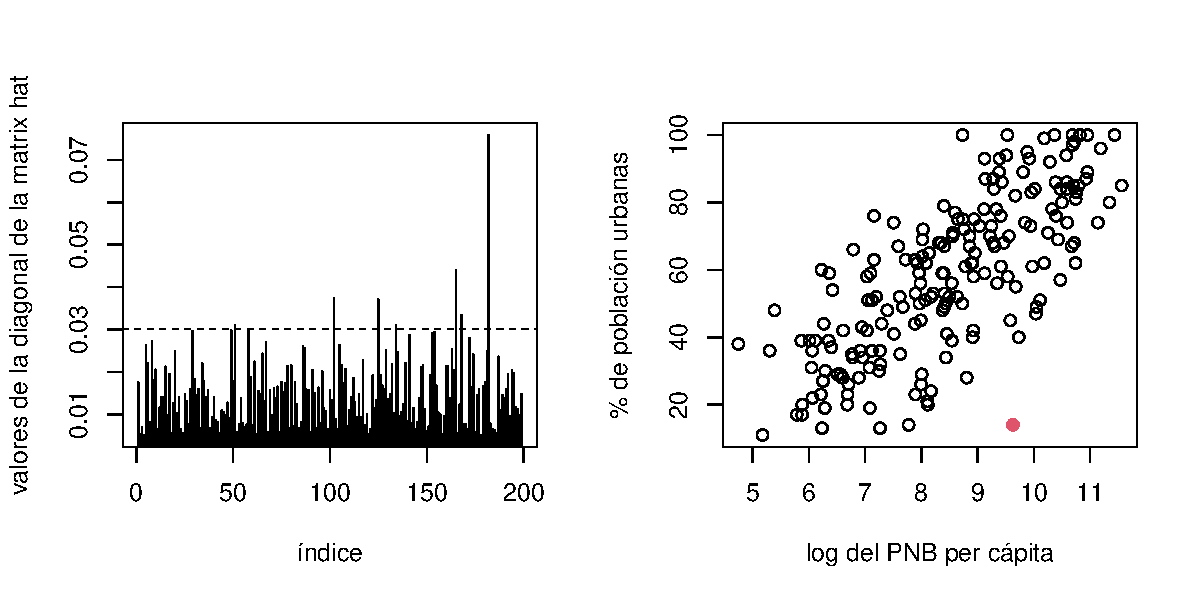
\includegraphics{MLG1_files/figure-latex/Un11Hdiag-1} 

}

\caption{Datos de la ONU. (a) Valores de la diagonal de lam matriz hat. (b) Diagrama de dispersión de las covariables (derecha). El punto rojo indica a Trinidad y Tobago.}\label{fig:Un11Hdiag}
\end{figure}

En laFigura \ref{fig:Un11Hdiag}(b) podemos observar que Trinidad y Tobago tiene un porcentaje muy pequeño de población en áreas urbanas y valor del PNB per cápita relativamente alto. Por esta razón el valor \(h_{ii}\) asociado es alto.

La Figura \ref{fig:Un11valAtip} muestra los valores de la diagonal de \(\boldsymbol H\) contra los residuos estudentizados. Aquí vemos que aunque Trinidad y Tobago tiene un valor \(h_{ii}\) alto, el R-Student asociado es bajo. Por lo que no se puede considerar como un punto influyente. Por el contrario, Guinea Ecuatorial y Corea del Norte presentan ambos valores altos (residuos y \(h_{ii}\)), por lo que se pueden considerar como puntos influyentes. Las observaciones que tienen residuos altos pero valores \(h_{ii}\) bajos se consideran como atípicos.

\begin{Shaded}
\begin{Highlighting}[]
\NormalTok{rstud.UN11 }\OtherTok{=}\NormalTok{ res.UN11}\SpecialCharTok{*}\FunctionTok{sqrt}\NormalTok{( (}\DecValTok{199{-}3{-}1}\NormalTok{)}\SpecialCharTok{/}\NormalTok{(}\DecValTok{199{-}3}\SpecialCharTok{{-}}\NormalTok{res.UN11}\SpecialCharTok{\^{}}\DecValTok{2}\NormalTok{) )}
\FunctionTok{plot}\NormalTok{(hii,rstud.UN11,}\AttributeTok{ylab=}\StringTok{\textquotesingle{}r Student\textquotesingle{}}\NormalTok{,}
     \AttributeTok{xlab=}\StringTok{\textquotesingle{}valores de la diagonal de la matrix hat\textquotesingle{}}\NormalTok{)}
\FunctionTok{abline}\NormalTok{(}\AttributeTok{h=}\DecValTok{0}\NormalTok{,}\AttributeTok{lty=}\DecValTok{2}\NormalTok{)}
\FunctionTok{abline}\NormalTok{(}\AttributeTok{h=} \FunctionTok{c}\NormalTok{(}\SpecialCharTok{{-}}\DecValTok{1}\NormalTok{,}\DecValTok{1}\NormalTok{)}\SpecialCharTok{*}\FunctionTok{qt}\NormalTok{(}\FloatTok{0.975}\NormalTok{,}\DecValTok{199{-}3{-}1}\NormalTok{),}\AttributeTok{lty=}\DecValTok{2}\NormalTok{)}
\FunctionTok{abline}\NormalTok{(}\AttributeTok{v=}\DecValTok{2}\SpecialCharTok{*}\DecValTok{3}\SpecialCharTok{/}\DecValTok{199}\NormalTok{,}\AttributeTok{lty=}\DecValTok{2}\NormalTok{)}
\FunctionTok{text}\NormalTok{(hii[Names}\SpecialCharTok{==}\StringTok{"Trinidad and Tobago"}\NormalTok{],}
\NormalTok{     rstud.UN11[Names}\SpecialCharTok{==}\StringTok{\textquotesingle{}Trinidad and Tobago\textquotesingle{}}\NormalTok{],}\StringTok{\textquotesingle{}Trinidad y Tobago\textquotesingle{}}\NormalTok{,}\AttributeTok{pos=}\DecValTok{2}\NormalTok{,}\AttributeTok{cex=}\FloatTok{0.8}\NormalTok{)}
\FunctionTok{text}\NormalTok{(hii[Names}\SpecialCharTok{==}\StringTok{"Equatorial Guinea"}\NormalTok{],}
\NormalTok{     rstud.UN11[Names}\SpecialCharTok{==}\StringTok{\textquotesingle{}Equatorial Guinea\textquotesingle{}}\NormalTok{],}\StringTok{\textquotesingle{}Guinea Ecuatorial\textquotesingle{}}\NormalTok{,}\AttributeTok{pos=}\DecValTok{4}\NormalTok{,}\AttributeTok{cex=}\FloatTok{0.8}\NormalTok{)}
\FunctionTok{text}\NormalTok{(hii[Names}\SpecialCharTok{==}\StringTok{"North Korea"}\NormalTok{],}
\NormalTok{     rstud.UN11[Names}\SpecialCharTok{==}\StringTok{\textquotesingle{}North Korea\textquotesingle{}}\NormalTok{],}\StringTok{\textquotesingle{}Corea del Norte\textquotesingle{}}\NormalTok{,}\AttributeTok{pos=}\DecValTok{4}\NormalTok{,}\AttributeTok{cex=}\FloatTok{0.8}\NormalTok{)}
\FunctionTok{text}\NormalTok{(hii[Names}\SpecialCharTok{==}\StringTok{"Somalia"}\NormalTok{],}
\NormalTok{     rstud.UN11[Names}\SpecialCharTok{==}\StringTok{\textquotesingle{}Somalia\textquotesingle{}}\NormalTok{],}\StringTok{\textquotesingle{}Somalia\textquotesingle{}}\NormalTok{,}\AttributeTok{pos=}\DecValTok{4}\NormalTok{,}\AttributeTok{cex=}\FloatTok{0.8}\NormalTok{)}
\FunctionTok{text}\NormalTok{(hii[Names}\SpecialCharTok{==}\StringTok{"Bosnia and Herzegovina"}\NormalTok{],}
\NormalTok{     rstud.UN11[Names}\SpecialCharTok{==}\StringTok{\textquotesingle{}Bosnia and Herzegovina\textquotesingle{}}\NormalTok{],}\StringTok{\textquotesingle{}Bosnia y Herz.\textquotesingle{}}\NormalTok{,}\AttributeTok{pos=}\DecValTok{4}\NormalTok{,}\AttributeTok{cex=}\FloatTok{0.8}\NormalTok{)}
\end{Highlighting}
\end{Shaded}

\begin{figure}

{\centering 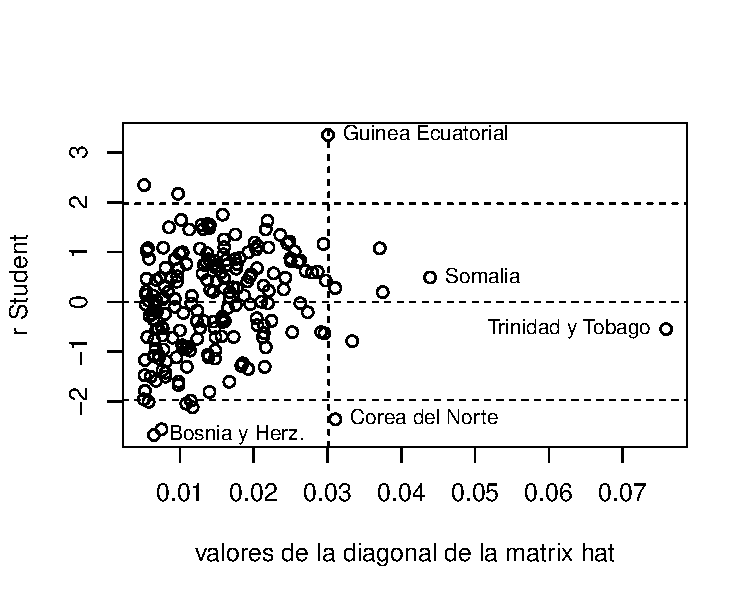
\includegraphics{MLG1_files/figure-latex/Un11valAtip-1} 

}

\caption{Datos de la ONU. Gráfico de valores influyentes}\label{fig:Un11valAtip}
\end{figure}
\rule{\textwidth}{0.4pt}

\hypertarget{medidas-de-influencia}{%
\subsubsection{Medidas de influencia}\label{medidas-de-influencia}}

El procedimiento para determinar si un punto es influyente se puede hacer evaluando los cambios que ocurren en el modelo ajustado cuando se elimina dicha observación.

Por ejemplo, la Figura \ref{fig:Un11valAtipElim} muestra cuanto cambian las estimaciones de \(\beta_{1}\) y \(\beta_{2}\) al eliminar un país a la vez. Aquí vemos que los cambios mas grandes ocurren cuando se eliminan a Guinea Ecuatorial o a Corea del Norte. Mientras que los países que identificamos como puntos de balanceo (Trinidad y Tobago y Somalia) o atípicos (Bosnia y Herzegovina) no tienen mucha influencia sobre las estimaciones.
\ldots.

\begin{figure}

{\centering 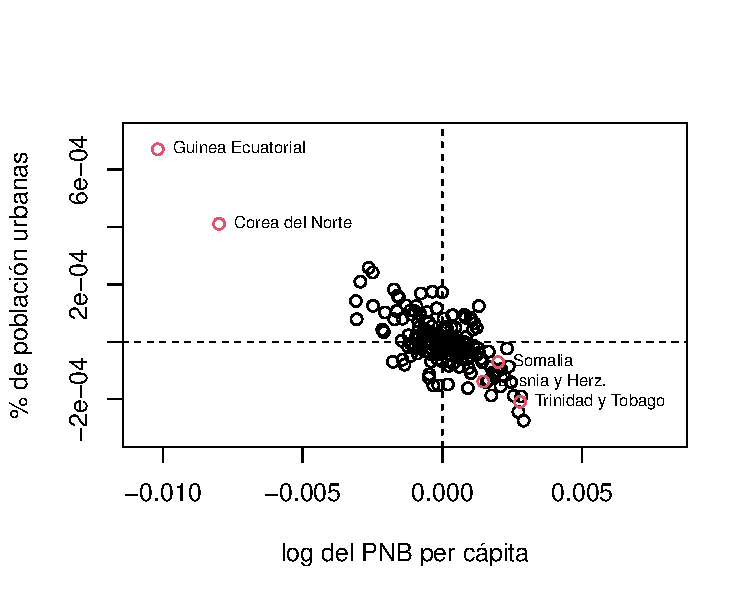
\includegraphics{MLG1_files/figure-latex/Un11valAtipElim-1} 

}

\caption{Datos de la ONU. Diferencias entre las estimaciones con todos los datos y las estimaciones obtenidas al eliminar una observación a la vez}\label{fig:Un11valAtipElim}
\end{figure}

De igual forma se podría evaluar cuanto cambian las estimaciones de \(E(y|\boldsymbol x_{i})\) o las varianzas de los coeficientes \(V(\beta_{j})\) al eliminar observaciones una a una.

A continuación se presentan algunos indicadores estadísticos para detectar puntos influyentes:

\hypertarget{distancia-de-cook}{%
\paragraph{Distancia de Cook}\label{distancia-de-cook}}

Esta es una medida de la distancia entre las estimaciones por MCO basado en los \(n\) puntos (\(\hat{\boldsymbol \beta}\)), y el estimado obtenido eliminando el \(i\)-ésimo punto (\(\hat{\boldsymbol \beta}_{(i)}\)). Es decir que es un indicador global de cuanto cambian todas las estimaciones de los coeficientes de regresión en conjunto. Esta medida se expresa de la siguiente forma:

\begin{equation}
\begin{split}
D_{i} &= \frac{(\hat{\boldsymbol \beta}_{(i)}-\hat{\boldsymbol \beta})'\boldsymbol X'\boldsymbol X(\hat{\boldsymbol \beta}_{(i)}-\hat{\boldsymbol \beta})'}{p \hat{\sigma}^{2}}   \\
      &= \frac{(\hat{\boldsymbol y}_{(i)} - \hat{\boldsymbol y} )'(\hat{\boldsymbol y}_{(i)} - \hat{\boldsymbol y} )}{p\hat{\sigma}^{2}} = \frac{r_{i}^{2}}{p}\frac{h_{ii}}{1-h_{ii}}, \qquad i=1,2,\ldots,n.
\end{split} \nonumber
\end{equation}

Aquí podemos observar que \(D_{i}\) consta de dos componentes, uno asociado a el residuo \((r_{i})\) y otro a la distancia del vector \(\boldsymbol x_{i}\) al centroide de la matriz de las covariables. Ambos (o alguno de ellos) puede contribuir a valores altos de este indicador.

Entonces, los puntos asociados a valores altos de \(D_{i}\) tienen gran influencia sobre la estimación de \(\boldsymbol \beta\) por MCO. Se considera como un punto influyente si tiene asociado un \(D_{i} > 4/n\) (algunos textos sugieren \(D_{i} > 1\)).

\hypertarget{dfbetas}{%
\paragraph{DFBETAS}\label{dfbetas}}

Esta medida indica cuánto cambia el coeficiente de regresión \(\hat{\beta}_{j}\), en unidades de desviaciones estándar, si se omitiera la \(i\)-ésima observación. Se calcula como:
\[
DFBETAS_{(i,j)} = \frac{\hat{\beta}_{j} - \hat{\beta}_{j(i)}}{\hat{\sigma}^{2}_{(i)}C_{jj}} = \frac{r_{(j,i)}}{\sqrt{\boldsymbol r_{j}'\boldsymbol r_{j}}}\frac{t_{i}}{\sqrt{1-h_{ii}}},
\]

donde \(C_{jj}\) es el \(j\)-ésimo valor de la diagonal de \((\boldsymbol X'\boldsymbol X)^{2}\). \(\boldsymbol r_{j}\) es la \(j\)-ésima fila de \(\boldsymbol R=(\boldsymbol X'\boldsymbol X)^{-1}\boldsymbol X\).

Un valor grande de \(DFBETAS_{(j,i)}\) indica que la observación \(i\) tiene gran influencia sobre el \(j\)-ésimo coeficiente de regresión. Se sugiere que si \(|DFBETAS_{(j,i)}| > 2/\sqrt{n}\) es necesario examinar la \(i\)-ésima observación.

\hypertarget{dffits}{%
\paragraph{DFFITS}\label{dffits}}

Una medida que indica la influencia de la observación \(i\)-ésima sobre el valor ajustado (\(\hat{y}_{i}\)). Esta se calcula así:

\[
DFFITS_{i} = \frac{\hat{y}_{i} - \hat{y}_{(i)}}{\hat{\sigma}_{(i)}^{2}h_{ii}} = \sqrt{ \frac{h_{ii}}{1-h_{ii}} }t_{i}.
\]

El \(DFFITS_{i}\) puede ser grande si el dato es atípico (\(t_{i}\) grande) o si el dato tiene gran balanceo (\(h_{ii}\) grande). Se sugiere que si \(|DFFITS_{(j,i)}| > 2\sqrt{p/n}\) es necesario examinar la \(i\)-ésima observación.

\hypertarget{covratio}{%
\paragraph{COVRATIO}\label{covratio}}

Los diagnósticos anteriores permiten ver el efecto de las observaciones sobre \(\hat{\boldsymbol \beta}\) o \(\hat{\boldsymbol y}\). Pero no proporcionan información sobre la precisión general de la estimación. Una medida global de la precisión es la varianza generalizada:

\[ GV(\hat{\boldsymbol \beta}) = | Var(\hat {\boldsymbol \beta}) | = |\sigma^{2}(\boldsymbol X'\boldsymbol X)^{-1}|.\]

Para determinar la influencia de la \(i\)-ésima observación en la precisión de la estimación se define la razón de covarianzas:

\[
COVRATIO_{i} = \frac{|(\boldsymbol X'_{(i)}\boldsymbol X_{(i)})^{-1}\hat{\sigma}_{(i)}^{2}|}{| (\boldsymbol X'\boldsymbol X)^{-1}\hat{\sigma}^{2} |}= \left( \frac{S^{2}_{(i)}}{S^{2}} \right)^{p} \left( \frac{1}{1-h_{ii}} \right).
\]

Si \(COVRATIO_{i} > 1 + 3p/n\) o \(COVRATIO_{i} > 1 - 3p/n\) se debería considerar a la \(i\)-ésima observación como influyente para la precisión de \(\widehat{\boldsymbol \beta}\).

\rule{\textwidth}{0.4pt}

\hypertarget{datos-de-la-onu---medidas-de-influencia}{%
\paragraph*{Datos de la ONU - medidas de influencia}\label{datos-de-la-onu---medidas-de-influencia}}
\addcontentsline{toc}{paragraph}{Datos de la ONU - medidas de influencia}

En R las medidas de influencia se pueden calcular usando la función \texttt{influence.measures}. Aunque también se pueden calcular cada indicador de forma independiente.

La distancia de Cook se observa en la Figura \ref{fig:Un11Cook}. Aquí vemos que Guinea Ecuatorial y Corea del Norte son los países que más influyen en las estimaciones de los parámetros del modelo. Lo demás países presentan valores de la distancia de Cook mucho más bajos. Note que aunque observamos que Trinidad y Tobago es un punto de balanceo, este país no es influyente (valor de la distancia de Cook de \(0.0082\)).

\begin{Shaded}
\begin{Highlighting}[]
\NormalTok{CD.UN11 }\OtherTok{=} \FunctionTok{cooks.distance}\NormalTok{(mod.UN11)}
\NormalTok{OrderCD.UN11 }\OtherTok{=} \FunctionTok{order}\NormalTok{(CD.UN11,}\AttributeTok{decreasing =}\NormalTok{ T)}
\FunctionTok{plot}\NormalTok{(CD.UN11,}\AttributeTok{type=}\StringTok{\textquotesingle{}h\textquotesingle{}}\NormalTok{,}\AttributeTok{ylab =} \StringTok{\textquotesingle{}distancia de Cook\textquotesingle{}}\NormalTok{,}\AttributeTok{xlab=}\StringTok{\textquotesingle{}índice\textquotesingle{}}\NormalTok{)}
\FunctionTok{text}\NormalTok{(OrderCD.UN11[}\DecValTok{1}\SpecialCharTok{:}\DecValTok{2}\NormalTok{],CD.UN11[OrderCD.UN11[}\DecValTok{1}\SpecialCharTok{:}\DecValTok{2}\NormalTok{]],Names[OrderCD.UN11[}\DecValTok{1}\SpecialCharTok{:}\DecValTok{2}\NormalTok{]],}\AttributeTok{pos=}\DecValTok{4}\NormalTok{,}\AttributeTok{cex=}\FloatTok{0.6}\NormalTok{)}
\FunctionTok{abline}\NormalTok{(}\AttributeTok{h=}\DecValTok{4}\SpecialCharTok{/}\DecValTok{199}\NormalTok{,}\AttributeTok{lty=}\DecValTok{2}\NormalTok{)}
\end{Highlighting}
\end{Shaded}

\begin{figure}

{\centering 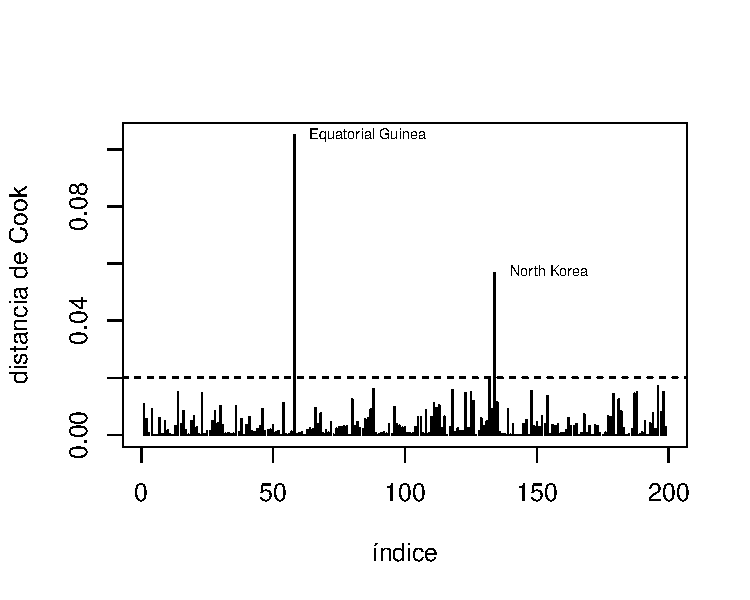
\includegraphics{MLG1_files/figure-latex/Un11Cook-1} 

}

\caption{Datos de la ONU. Distancia de Cook.}\label{fig:Un11Cook}
\end{figure}

Ya identificamos que Guinea Ecuatorial y Corea del Norte son influyentes y pueden afectar considerablemente las estimaciones de los coeficientes de regresión. Pero esta influencia puede ser solamente sobre algún o algunos parámetros. Para ver la influencia sobre cada parámetro, la Figura \ref{fig:UNdataDfBetas} muestra los DFBETAS para los coeficientes \(\beta_{1}\) y \(\beta_{2}\). En ambos gráficos podemos ver que estos dos países son influyentes para ambos parámetros. También se pude observar que otros pocos países tienen cierta influencia en la estimación de \(\beta_{2}\), aunque los valores de los DFBETAS están muy cerca de los puntos de corte.

\begin{Shaded}
\begin{Highlighting}[]
\NormalTok{DFBetas.UN11 }\OtherTok{=} \FunctionTok{dfbetas}\NormalTok{(mod.UN11)}
\NormalTok{OrderDB1.UN11 }\OtherTok{=} \FunctionTok{order}\NormalTok{(}\FunctionTok{abs}\NormalTok{(DFBetas.UN11[,}\DecValTok{2}\NormalTok{]),}\AttributeTok{decreasing =}\NormalTok{ T)}
\NormalTok{OrderDB2.UN11 }\OtherTok{=} \FunctionTok{order}\NormalTok{(}\FunctionTok{abs}\NormalTok{(DFBetas.UN11[,}\DecValTok{3}\NormalTok{]),}\AttributeTok{decreasing =}\NormalTok{ T)}
\FunctionTok{par}\NormalTok{(}\AttributeTok{mfrow=}\FunctionTok{c}\NormalTok{(}\DecValTok{1}\NormalTok{,}\DecValTok{2}\NormalTok{))}
\FunctionTok{plot}\NormalTok{(DFBetas.UN11[,}\DecValTok{2}\NormalTok{],}\AttributeTok{ylab=}\FunctionTok{quote}\NormalTok{(}\StringTok{\textquotesingle{}DFBETA\textquotesingle{}}\SpecialCharTok{\textasciitilde{}}\NormalTok{(beta[}\DecValTok{1}\NormalTok{])),}\AttributeTok{xlab=}\StringTok{\textquotesingle{}índice\textquotesingle{}}\NormalTok{,}\AttributeTok{main=}\StringTok{\textquotesingle{}(a)\textquotesingle{}}\NormalTok{)}
\FunctionTok{text}\NormalTok{(OrderDB1.UN11[}\DecValTok{1}\SpecialCharTok{:}\DecValTok{2}\NormalTok{],DFBetas.UN11[OrderDB1.UN11[}\DecValTok{1}\SpecialCharTok{:}\DecValTok{2}\NormalTok{],}\DecValTok{2}\NormalTok{],}
\NormalTok{     Names[OrderDB1.UN11[}\DecValTok{1}\SpecialCharTok{:}\DecValTok{2}\NormalTok{]],}\AttributeTok{pos=}\DecValTok{4}\NormalTok{,}\AttributeTok{cex=}\FloatTok{0.6}\NormalTok{)}
\FunctionTok{abline}\NormalTok{(}\AttributeTok{h =} \FunctionTok{c}\NormalTok{(}\SpecialCharTok{{-}}\DecValTok{1}\NormalTok{,}\DecValTok{1}\NormalTok{)}\SpecialCharTok{*}\DecValTok{2}\SpecialCharTok{/}\FunctionTok{sqrt}\NormalTok{(}\DecValTok{199}\NormalTok{),}\AttributeTok{lty=}\DecValTok{2}\NormalTok{)}
\FunctionTok{plot}\NormalTok{(DFBetas.UN11[,}\DecValTok{3}\NormalTok{],}\AttributeTok{ylab =} \FunctionTok{quote}\NormalTok{(}\StringTok{\textquotesingle{}DFBETA\textquotesingle{}}\SpecialCharTok{\textasciitilde{}}\NormalTok{(beta[}\DecValTok{2}\NormalTok{])),}\AttributeTok{xlab=}\StringTok{\textquotesingle{}índice\textquotesingle{}}\NormalTok{,}\AttributeTok{main=}\StringTok{\textquotesingle{}(b)\textquotesingle{}}\NormalTok{)}
\FunctionTok{text}\NormalTok{(OrderDB2.UN11[}\DecValTok{1}\SpecialCharTok{:}\DecValTok{2}\NormalTok{],DFBetas.UN11[OrderDB2.UN11[}\DecValTok{1}\SpecialCharTok{:}\DecValTok{2}\NormalTok{],}\DecValTok{3}\NormalTok{],}
\NormalTok{     Names[OrderDB2.UN11[}\DecValTok{1}\SpecialCharTok{:}\DecValTok{2}\NormalTok{]],}\AttributeTok{pos=}\DecValTok{4}\NormalTok{,}\AttributeTok{cex=}\FloatTok{0.6}\NormalTok{)}
\FunctionTok{abline}\NormalTok{(}\AttributeTok{h =} \FunctionTok{c}\NormalTok{(}\SpecialCharTok{{-}}\DecValTok{1}\NormalTok{,}\DecValTok{1}\NormalTok{)}\SpecialCharTok{*}\DecValTok{2}\SpecialCharTok{/}\FunctionTok{sqrt}\NormalTok{(}\DecValTok{199}\NormalTok{),}\AttributeTok{lty=}\DecValTok{2}\NormalTok{)}
\end{Highlighting}
\end{Shaded}

\begin{figure}

{\centering 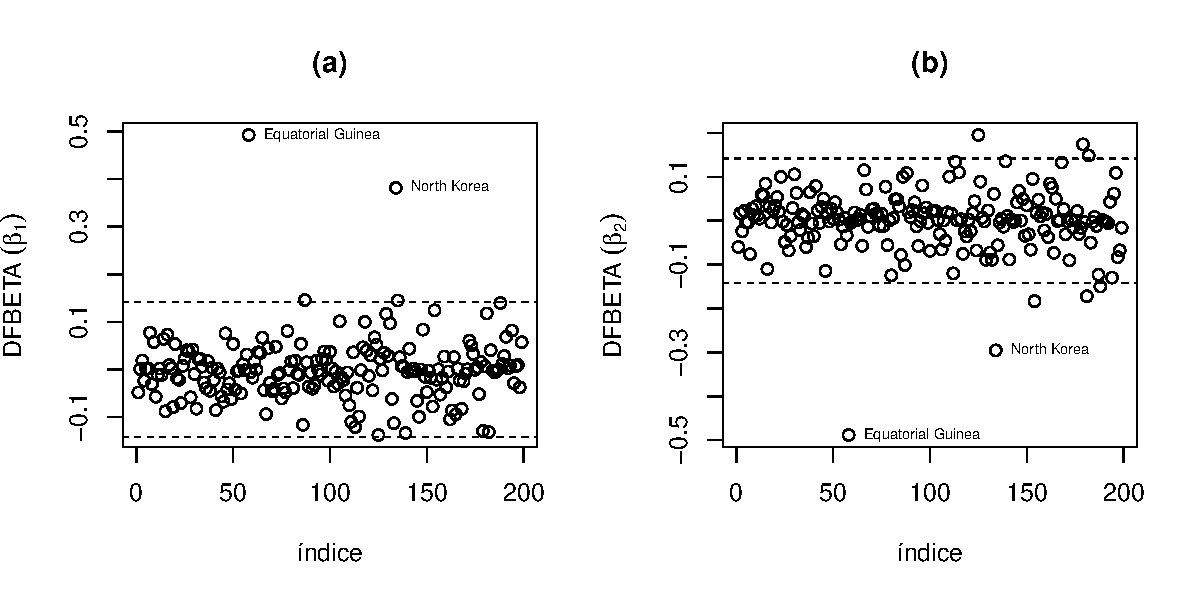
\includegraphics{MLG1_files/figure-latex/UNdataDfBetas-1} 

}

\caption{Datos de la ONU. DFBetas.}\label{fig:UNdataDfBetas}
\end{figure}

Los DFFITS y COVRATIO se observan en la Figura \ref{fig:UNdataOtros}. A partir de los DFFITS se puede concluir que Guinea Ecuatorial y Corea del Norte también tienen gran influencia sobre las predicciones. A partir de los COVRATIO vemos que Trinidad y Tobago, Guinea Ecuatorial, Bosnia y Herzegovina, y Moldavia tienen gran influencia en la varianza de las estimaciones de los coeficientes de regresión. Note que aunque Corea del Norte fue influyente para las estimaciones, este país no influye en la varianza de estas.

\begin{Shaded}
\begin{Highlighting}[]
\NormalTok{DFfits.UN11 }\OtherTok{=} \FunctionTok{dffits}\NormalTok{(mod.UN11)}
\NormalTok{OrderDFF.UN11 }\OtherTok{=} \FunctionTok{order}\NormalTok{(}\FunctionTok{abs}\NormalTok{(DFfits.UN11),}\AttributeTok{decreasing =}\NormalTok{ T)}

\NormalTok{Covratio.UN11 }\OtherTok{=} \FunctionTok{covratio}\NormalTok{(mod.UN11)}
\NormalTok{OrderCR.UN11 }\OtherTok{=} \FunctionTok{order}\NormalTok{(}\FunctionTok{abs}\NormalTok{(}\DecValTok{1}\SpecialCharTok{{-}}\NormalTok{Covratio.UN11),}\AttributeTok{decreasing =}\NormalTok{ T)}
\FunctionTok{par}\NormalTok{(}\AttributeTok{mfrow=}\FunctionTok{c}\NormalTok{(}\DecValTok{1}\NormalTok{,}\DecValTok{2}\NormalTok{))}
\FunctionTok{plot}\NormalTok{(DFfits.UN11,}\AttributeTok{ylab=}\StringTok{\textquotesingle{}DFFITS\textquotesingle{}}\NormalTok{,}\AttributeTok{xlab=}\StringTok{\textquotesingle{}índice\textquotesingle{}}\NormalTok{,}\AttributeTok{main=}\StringTok{\textquotesingle{}(a)\textquotesingle{}}\NormalTok{)}
\FunctionTok{text}\NormalTok{(OrderDFF.UN11[}\DecValTok{1}\SpecialCharTok{:}\DecValTok{2}\NormalTok{],DFfits.UN11[OrderDFF.UN11[}\DecValTok{1}\SpecialCharTok{:}\DecValTok{2}\NormalTok{]],}
\NormalTok{     Names[OrderDFF.UN11[}\DecValTok{1}\SpecialCharTok{:}\DecValTok{2}\NormalTok{]],}\AttributeTok{pos=}\DecValTok{4}\NormalTok{,}\AttributeTok{cex=}\FloatTok{0.6}\NormalTok{)}
\FunctionTok{abline}\NormalTok{(}\AttributeTok{h =} \FunctionTok{c}\NormalTok{(}\SpecialCharTok{{-}}\DecValTok{1}\NormalTok{,}\DecValTok{1}\NormalTok{)}\SpecialCharTok{*}\DecValTok{2}\SpecialCharTok{*}\FunctionTok{sqrt}\NormalTok{(}\DecValTok{3}\SpecialCharTok{/}\DecValTok{199}\NormalTok{),}\AttributeTok{lty=}\DecValTok{2}\NormalTok{)}
\FunctionTok{plot}\NormalTok{(Covratio.UN11,}\AttributeTok{ylab =} \StringTok{\textquotesingle{}COVRATIO\textquotesingle{}}\NormalTok{,}\AttributeTok{xlab=}\StringTok{\textquotesingle{}índice\textquotesingle{}}\NormalTok{,}\AttributeTok{main=}\StringTok{\textquotesingle{}(b)\textquotesingle{}}\NormalTok{)}
\FunctionTok{text}\NormalTok{(OrderCR.UN11[}\DecValTok{1}\SpecialCharTok{:}\DecValTok{4}\NormalTok{],Covratio.UN11[OrderCR.UN11[}\DecValTok{1}\SpecialCharTok{:}\DecValTok{4}\NormalTok{]],}
\NormalTok{     Names[OrderCR.UN11[}\DecValTok{1}\SpecialCharTok{:}\DecValTok{4}\NormalTok{]],}\AttributeTok{pos=}\FunctionTok{c}\NormalTok{(}\DecValTok{4}\NormalTok{,}\DecValTok{2}\NormalTok{,}\DecValTok{4}\NormalTok{,}\DecValTok{4}\NormalTok{),}\AttributeTok{cex=}\FloatTok{0.6}\NormalTok{)}
\FunctionTok{abline}\NormalTok{(}\AttributeTok{h =} \DecValTok{1}\SpecialCharTok{+}\FunctionTok{c}\NormalTok{(}\SpecialCharTok{{-}}\DecValTok{1}\NormalTok{,}\DecValTok{1}\NormalTok{)}\SpecialCharTok{*}\DecValTok{3}\SpecialCharTok{*}\DecValTok{3}\SpecialCharTok{/}\DecValTok{199}\NormalTok{,}\AttributeTok{lty=}\DecValTok{2}\NormalTok{)}
\end{Highlighting}
\end{Shaded}

\begin{figure}

{\centering 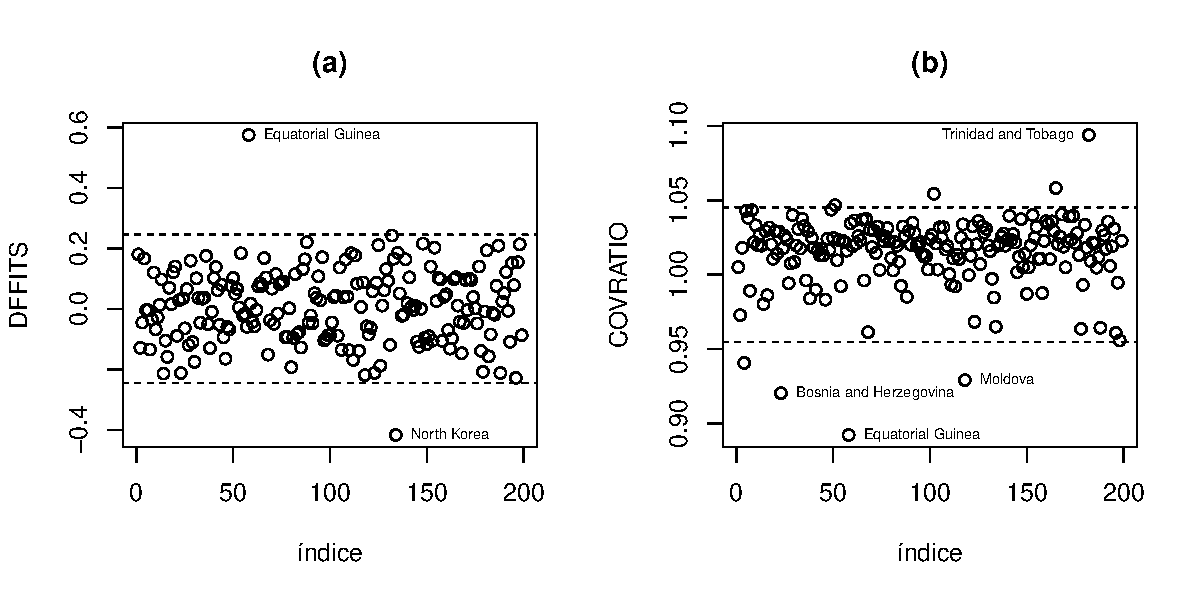
\includegraphics{MLG1_files/figure-latex/UNdataOtros-1} 

}

\caption{Datos de la ONU. DFFITS y COVRATIO.}\label{fig:UNdataOtros}
\end{figure}

A partir de estos indicadores encontramos que Guinea Ecuatorial y Corea del Norte son observaciones influyentes en la estimación del modelo \eqref{eq:modUN}. Particularmente, Guinea Ecuatorial tiene una tasa de fertilidad (4.98) muy superior a la estimada por el modelo. Esto se debe que los países con PNB y porcentaje de población urbana similares a este país tienen tasas de fertilidad más baja. Caso contrario pasa con Corea del Norte.

Para disminuir la influencia de estos países se pueden incorporar nuevas covariables dentro del modelo que ayuden a explicar estas discrepancias. Por ejemplo se podría ingresar una covariable asociada al continente.

\rule{\textwidth}{0.4pt}

\hypertarget{comentarios-finales-1}{%
\subsection{Comentarios finales}\label{comentarios-finales-1}}

\begin{itemize}
\tightlist
\item
  Dentro de la literatura hay muchos puntos de corte diferentes para los indicadores de observaciones influyentes. Esto es porque es difícil de determinar las distribuciones muestrales. Por lo que se recomienda verificar si hay algunas observaciones que tenga valores muy altos con respecto a los demás.
\item
  Las observaciones influyentes o atípicas se deben descartar si estas corresponden a errores de medición o si son inválidas (por ejemplo, si pertenecen a otra población).
\item
  Pero si las observaciones influyentes o atípicas son válidas, no hay justificación para eliminarla. Lo que se puede hacer es incluir nuevas covariables que puedan explicar mejor los datos y reducir la influencia de estas observaciones. En los datos de la ONU podríamos incluir covariables relacionadas con el continente.
\end{itemize}

  \bibliography{ModeloLineal.bib}

\end{document}
